\documentclass{article}
\usepackage{amsmath,amssymb,amsthm,kotex,mdframed,paralist}

\newcounter{num}
%\newcommand{\defi}[1]
%{\bigskip\noindent\refstepcounter{num}\textbf{정의 \arabic{num}) #1}\par}
%\newcommand{\theo}[1]
%{\bigskip\noindent\refstepcounter{num}\textbf{정리 \arabic{num}) #1}\par}
\newcommand{\exam}[1]
{\bigskip\noindent\refstepcounter{num}\textbf{예제 \arabic{num}) #1}\par}
\newcommand{\prob}[1]
{\bigskip\noindent\refstepcounter{num}\textbf{문제 \arabic{num}) #1}\par}
\newcommand{\summ}[1]
{\bigskip\noindent\refstepcounter{num}\textbf{요약 \arabic{num}) #1}\par}

\renewcommand{\figurename}{그림}
%\renewcommand{\proofname}{증명)}
\newcommand{\sol}{\par\bigskip\noindent{\bfseries풀이)}\par}
\newcommand{\ans}[1]{{\raggedleft\textbf{답 : }#1\par}}

%%%
\begin{document}

\title{영석 : 09 기말고사(1학년 1학기) 개념 요약}
\author{}
\date{\today}
\maketitle
\tableofcontents
\newpage

%%
\section{여러 가지 부등식}


\summ{}
\begin{enumerate}
\item
부등식의 양변에 같은 값을 더하거나 빼더라도 부등호의 방향은 바뀌지 않는다.
\item
부등식의 양변에 같은 값을 곱하거나 나눌 때에는, 곱하거나 나누는 수가 양수이면 부등호의 방향이 바뀌지 않고, 음수이면 부등호의 방향이 바뀐다.
\item
양수 \(a\)에 대해,
\begin{enumerate}
\item
\(|x|<a\)이면 \(-a<x<a\)이다.
\item
\(|x|>a\)이면 \(x<-a\) 또는 \(x>a\)이다.
\end{enumerate}
\item
이차부등식의 해는 다음과 같이 구한다(\(a>0\)).
\bigskip

\noindent
{\footnotesize
\begin{tabular}{p{0.24\textwidth}|p{0.24\textwidth}|p{0.24\textwidth}|p{0.24\textwidth}}
\hline
&\(D>0\)		&\(D=0\)	&\(D<0\)\\
\hline
\(y=ax^2+bx+c\)의 그래프
&\raisebox{-.5\height}{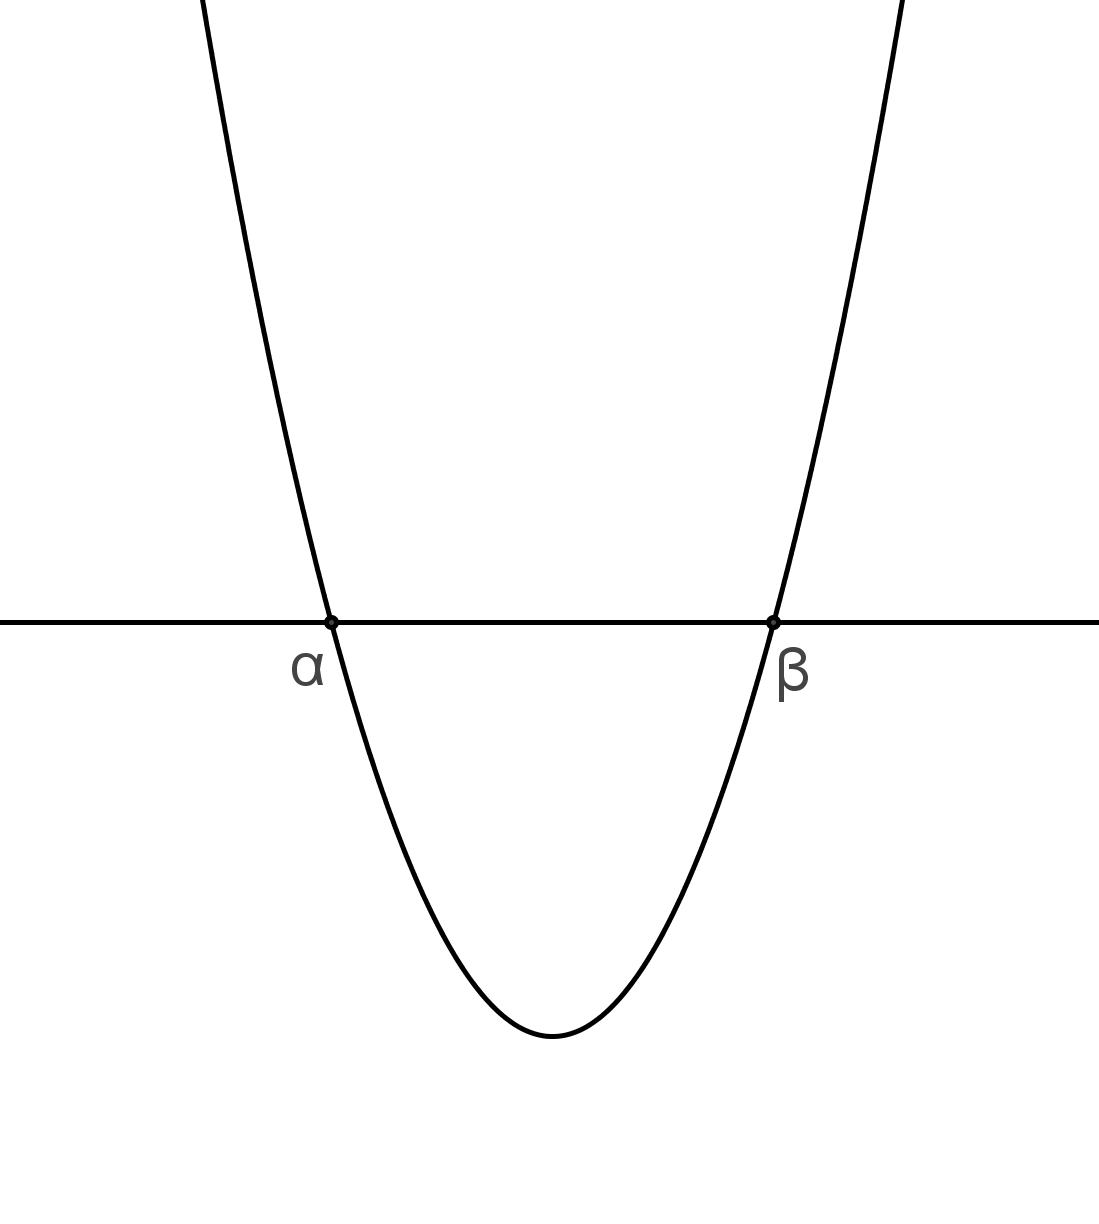
\includegraphics[width=0.24\textwidth]{1}}
&\raisebox{-.5\height}{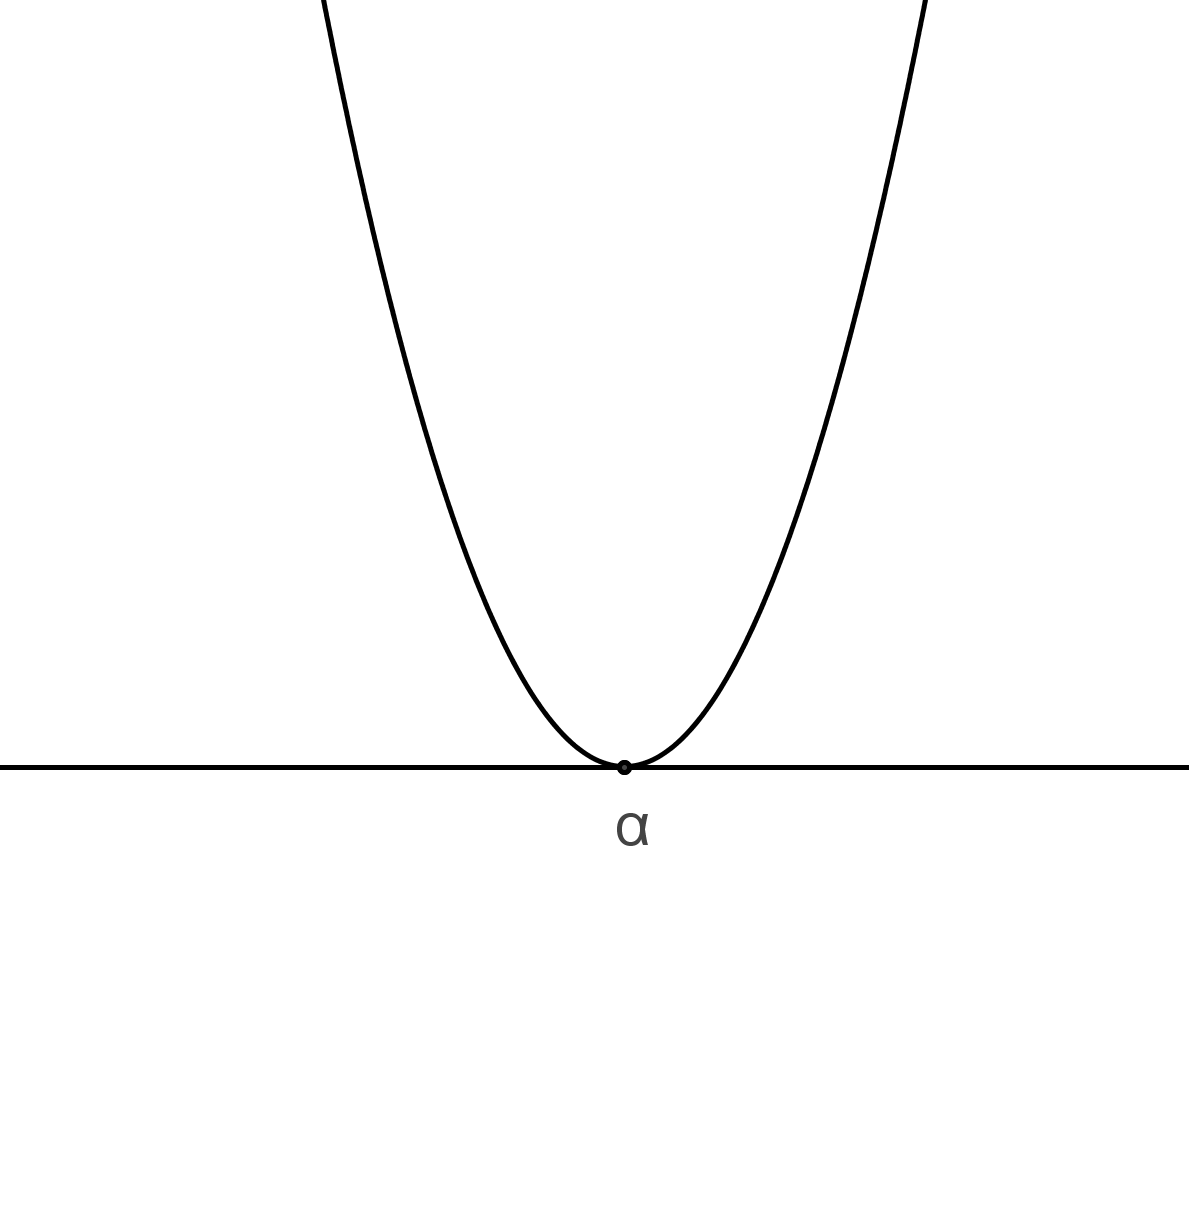
\includegraphics[width=0.24\textwidth]{2}}
&\raisebox{-.5\height}{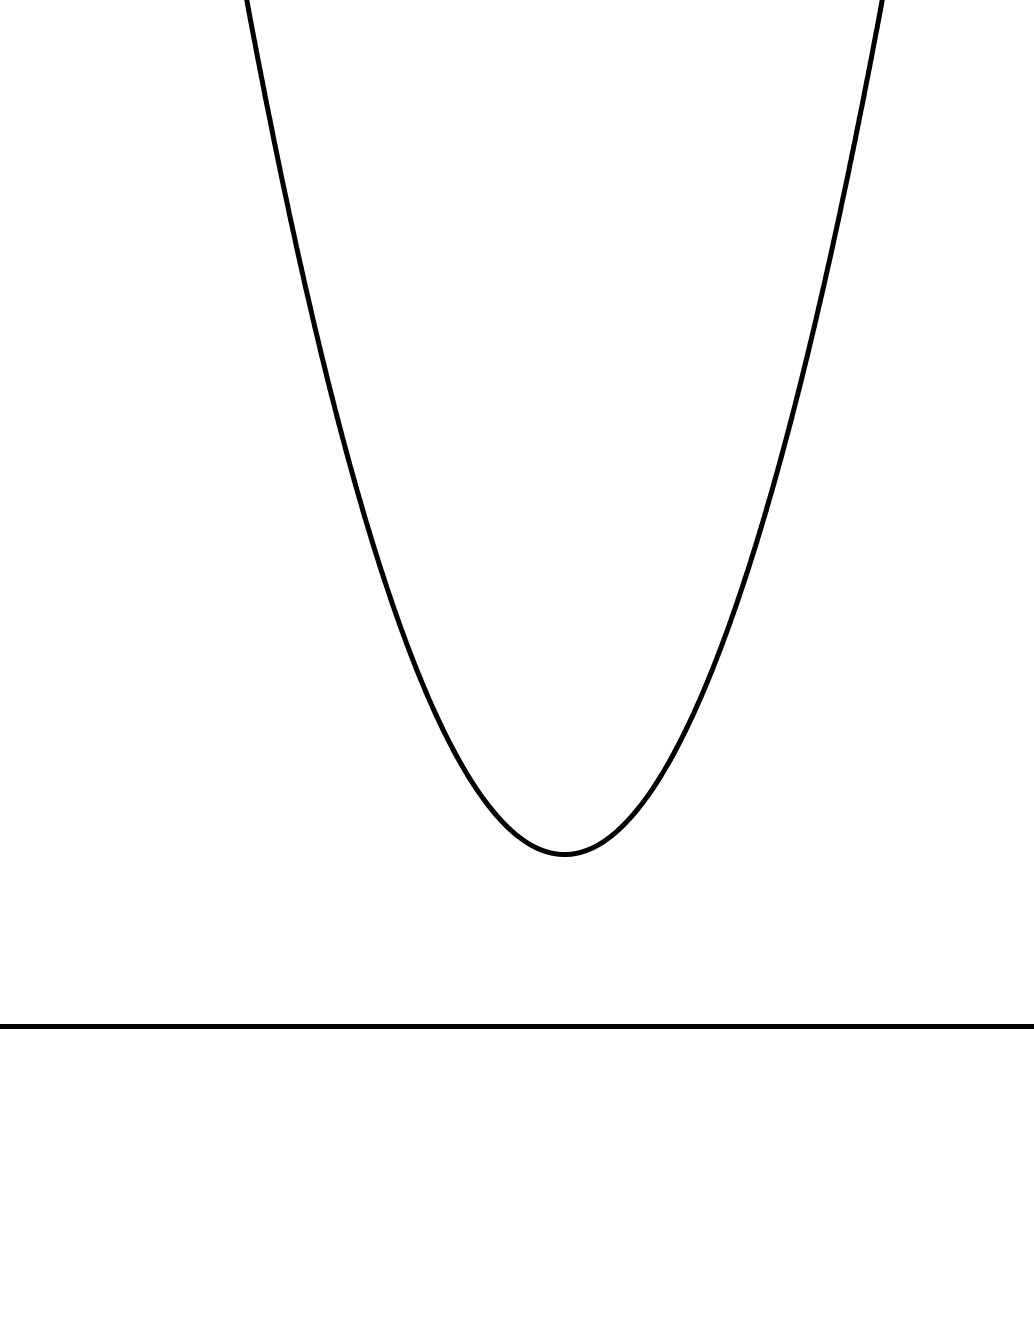
\includegraphics[width=0.24\textwidth]{3}}\\
\hline
\(ax^2+bx+c>0\)의 해
&\(x<\alpha\) 또는 \(x>\beta\)		&\(x\neq\alpha\)인 모든 실수	&모든 실수\\\hline
\(ax^2+bx+c\ge0\)의 해
&\(x\le\alpha\) 또는 \(x\ge\beta\)	&모든 실수					&모든 실수\\\hline
\(ax^2+bx+c<0\)의 해
&\(\alpha<x<\beta\)				&없다.					&없다.\\\hline
\(ax^2+bx+c\le0\)의 해
&\(\alpha\le x\le\beta\)			&\(x=\alpha\)				&없다.\\\hline
\end{tabular}
}\end{enumerate}

%
\exam{}
다음 부등식을 풀어라.\\
(1) \(3x<9\)\\
(2) \(6-3x\ge2(x+1)\)

\sol
(1) 양변을 \(3\)으로 나누면 \(x<3\)이다.

(2) 우변을 전개하면 \(6-3x\ge2x+2\)이고, 양변에서 \(6\)을 빼면 (\(6\)을 이항하면) \(-3x\ge2x-4\)이며, 다시 양변에서 \(2x\)를 빼면 \(-5x\ge-4\)가 된다.
마지막으로 양변을 \(-5\)로 나누면 \(x\le\frac45\)이다.

%
\prob{}
다음 부등식을 풀어라.\\
(1) \(3x-2<13\)\\
(2) \(x+2\ge-2x+5\)

\ans{(1) \(x<5\) (2) \(x\ge1\)}

%
\exam{}
부등식 \(|x-2|<3\)을 풀어라.
\sol
\(-3<x-2<3\)이 성립한다.
이는 \(-3<x-2\)와 \(x-2<3\)이 성립한다는 뜻이다.
각각을 정리하면 \(x>-1\), \(x<5\)가 되므로 \(-1<x<5\)이다.

%
\prob{}
다음 부등식을 풀어라.\\
(1) \(|x+3|>1\)\\
(2) \(|3x+2|<4\)\\
(3) \(|5-2x|\ge7\)\\
(4) \(|2x-1|\le3x+2\)

\ans{(1) \(x<-4\) 또는 \(x>-2\) (2) \(-2<x<\frac23\)\\
(3) \(x\le-1\) 또는 \(x\ge6\) (4) \(x\ge-\frac15\)}

%
\exam{}
다음 이차부등식을 풀어라.\\
(1) \(x^2-2x-3>0\)\\
(2) \(x^2-6x+9\ge0\)\\
(3) \(x^2+2x+2\le0\)
\sol
(1)
\(D=(-2)^2-4\times1\times(-3)>0\)이므로 \(y=x^2-2x-3\)은 \(x\)축과 두 점에서 만난다.
또 \(x^2-2x-3=(x+1)(x-3)\)이므로 만나는 두 점의 \(x\)좌표는 \(-1\)과 \(3\)이다.
따라서 \(y=x^2-2x-3\)의 그래프는 그림 \ref{y=x^2-2x-3}과 같이 나타난다.
그러므로 \(x<-1\) 또는 \(x>3\)이다.

\begin{figure}[h!]
\center
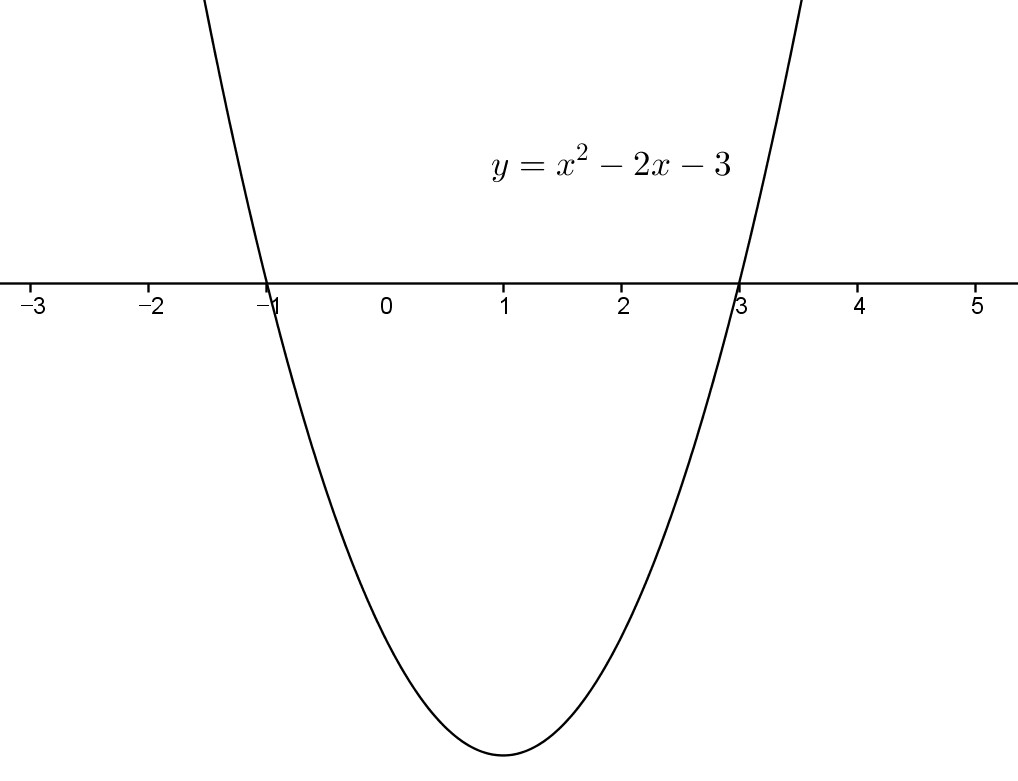
\includegraphics[width=0.4\textwidth]{y=x^2-2x-3}
\caption{\(y=x^2-2x-3\)의 그래프}
\label{y=x^2-2x-3}
\end{figure}

(2)
\(D=(-6)^2-4\times1\times9=0\)이므로 \(y=x^2-6x+9\)는 \(x\)축과 한 점에서 만난다(접한다).
또 \(x^2-6x+9=(x-3)^2\)이므로 만나는 점의 \(x\)좌표는 \(3\)이다.
따라서 \(y=x^2-6x+9\)의 그래프는 그림 \ref{y=x^2-6x+9}과 같이 나타난다.
그러므로 해는 모든 실수이다.

\begin{figure}[h!]
\center
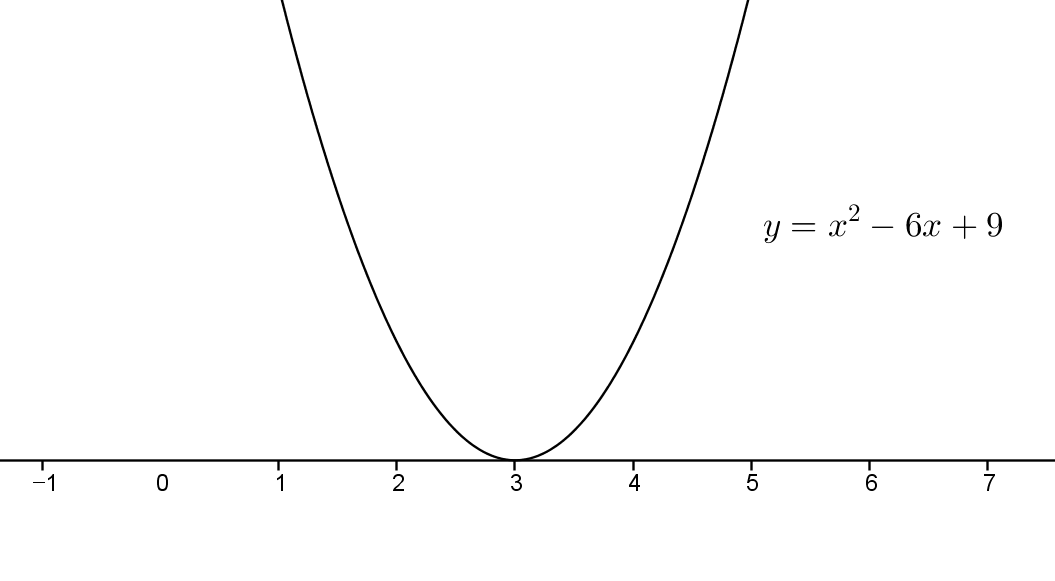
\includegraphics[width=0.4\textwidth]{y=x^2-6x+9}
\caption{\(y=x^2-6x+9\)의 그래프}
\label{y=x^2-6x+9}
\end{figure}

(3) \(D=2^2-4\times1\times2<0\)이므로 \(y=x^2+2x+2\)는 \(x\)축과 만나지 않는다.
따라서 \(y=x^2+2x+2\)의 그래프는 그림 \ref{y=x^2+2x+2}와 같이 나타난다.
그러므로 해는 없다.

\begin{figure}[h!]
\center
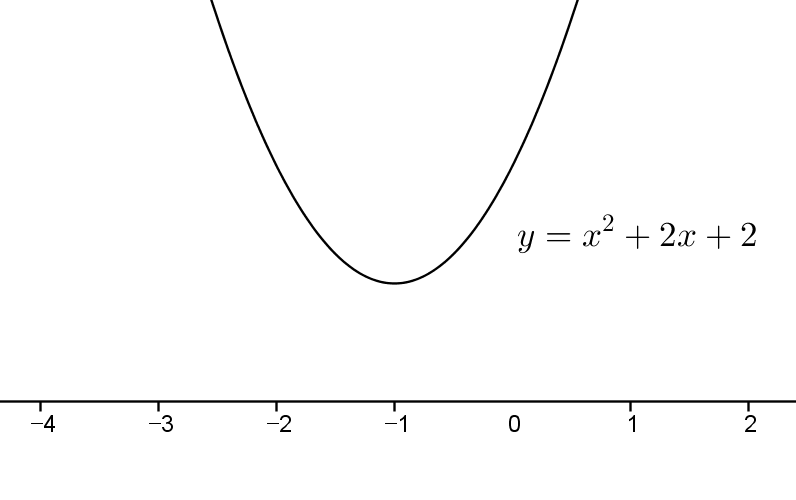
\includegraphics[width=0.4\textwidth]{y=x^2+2x+2}
\caption{\(y=x^2+2x+2\)의 그래프}
\label{y=x^2+2x+2}
\end{figure}

%
\prob{}
다음 이차부등식을 풀어라.\\
(1) \(x^2-x-2<0\)\\
(2) \(2x^2-3x+1\ge0\)\\
(3) \(-x^2+5x+6\ge0\)\\
(4) \(2x^2>3x+2\)\\
(5) \(x^2-2x+1>0\)\\
(6) \(x^2+10x+25\le0\)\\
(7) \(-4x^2+4x-1\le0\)\\
(8) \(10x\ge x^2+25\)\\
(9) \(x^2+3x+3\le0\)\\
(10) \(x^2+x+2>0\)\\
(11) \(-2x^2+5x-7\le0\)\\
(12) \(x^2<4x-5\)

\ans{
(1) \(-1<x<2\)
(2) \(x\le\frac12\) 또는 \(x\ge1\)\\
(3) \(-1\le x\le6\)
(4) \(x<-\frac12\) 또는 \(x>2\)\\
(5) \(x\neq1\)
(6) \(x=-5\)\\
(7) 모든 실수
(8) \(x=5\)\\
(9) 해는 없다.
(10) 모든 실수\\
(11) 모든 실수
(12) 해는 없다.
}


%%
\section{평면좌표}

%
\summ{}
\begin{enumerate}
\item
수직선 상의 두 점 \(A(x_1)\), \(B(x_2)\) 사이의 거리는 \(|x_1-x_2|\)이다.
\item
좌표 평면 위의 두 점 \(A(x_1,y_1)\), \(B(x_2,y_2)\) 사이의 거리는 \(\sqrt{(x_1-x_2)^2+(y_1-y_2)^2}\)이다.
\item
수직선 상의 두 점 \(A(x_1)\), \(B(x_2)\)에 대해 \(m:n\) 내분점 \(P\)와 외분점 \(Q\)의 좌표는 \(P=(\frac{mx_2+nx_1}{m+n})\), \(Q=(\frac{mx_2-nx_1}{m-n})\) 이다.
\item
좌표평면 상의 두 점 \(A(x_1,y_1)\), \(B(x_2,y_2)\)에 대한 \(m:n\) 내분점 \(P\)와 외분점 \(Q\)의 좌표는 \(P=(\frac{mx_2+nx_1}{m+n},\frac{my_2+ny_1}{m+n})\), \(Q=(\frac{mx_2-nx_1}{m-n},\frac{my_2-ny_1}{m-n})\) 이다.
\item
두 점 \(A(x_1,y_1)\), \(B(x_2,y_2)\)가 이루는 선분 \(AB\)의 중점 \(M\)의 좌표는
\(M=(\frac{x_1+x_2}2,\frac{y_1+y_2}2)\)
이다.
\item
세 점 \(A(x_1,y_1)\), \(B(x_2,y_2)\), \(C(x_3,y_3)\)가 이루는 삼각형 \(ABC\)의 무게중심 \(G\)의 좌표는
\(G=(\frac{x_1+x_2+x_3}3,\frac{y_1+y_2+y_3}3)\)
이다.
\end{enumerate}

%
\exam{}
다음 두 점 사이의 거리를 구하여라.\\
(1) \(A(0,0)\), \(B(3,4)\)\\
(2) \(A(-1,2)\), \(B(11,7)\)

\sol
(1) \(\overline{AB}=\sqrt{(0-3)^2+(0-4)^2}=\sqrt{25}=5\)

(2) \(\overline{AB}=\sqrt{(-1-11)^2+(2-7)^2}=\sqrt{169}=13\)

%
\prob{}
다음 두 점 사이의 거리를 구하여라.\\
(1) \(A(1,3)\), \(B(-2,4)\)\\
(2) \(A(0,0)\), \(B(1,-5)\)\\
(3) \(A(2,6)\), \(B(-1,-5)\)\\
(4) \(A(3,-3)\), \(B(4,4)\)

\ans{(1) \(\sqrt{10}\) (2) \(\sqrt{26}\) (3) \(\sqrt{130}\) (4) \(5\sqrt2\)}

%
\exam{}
세 점 \(A(-2,2)\), \(B(1,-4)\), \(C(4,5)\)를 꼭짓점으로 하는 삼각형 \(ABC\)는 어떤 삼각형인지 말하여라.

\sol
\begin{align*}
\overline{AB}&=\sqrt{3^2+6^2}=3\sqrt5,\\
\overline{BC}&=\sqrt{3^2+9^2}=3\sqrt{10},\\
\overline{CA}&=\sqrt{6^2+3^2}=3\sqrt5
\end{align*}
이므로 \(\overline{AB}=\overline{CA}\)이고 \(\overline{AB}^2+\overline{CA}^2=\overline{BC}^2\)이다.
따라서 삼각형 \(ABC\)는 \(\angle A=90^\circ\)인 직각이등변삼각형이다.

%
\prob{}
세 점 \(A(1,3)\), \(B(-1,-3)\), \(C(-3,-1)\)을 꼭짓점으로 하는 삼각형 \(ABC\)는 어떤 삼각형인지 말하여라.

\ans{\(\angle C=90^\circ\)인 직각삼각형}


%
\exam{}
두 점 \(A(5,3)\), \(B(-2,1)\)에 대하여 다음 점의 좌표를 구하여라.\\
(1) 선분 \(AB\)를 \(1:2\)로 내분하는 점\\
(2) 선분 \(AB\)를 \(1:2\)로 외분하는 점

\sol
(1) 내분점을 \(P\)라고 하면
\(P=(\frac{1\times(-2)+2\times5}{1+2},\frac{1\times1+2\times3}{1+2})=(\frac83,\frac73)\)

(2) 외분점을 \(Q\)라고 하면
\(Q=(\frac{1\times(-2)-2\times5}{1-2},\frac{1\times1-2\times3}{1-2})=(12,5)\)

%
\prob{}
다음 두 점 \(A\), \(B\)에 대하여 선분 \(AB\)를 \(4:3\)으로 내분하는 점과 \(4:3\)으로 외분하는 점의 좌표를 각각 구하여라.\\
(1) \(A(1,3)\), \(B(7,8)\)\\
(2) \(A(-3,6)\), \(B(5,-4)\)

\ans{
(1) 내분하는 점 : \((\frac{31}7,\frac{41}7)\), 외분하는 점 : \((25,23)\)\\
(2) 내분하는 점 : \((\frac{11}7,\frac27)\), 외분하는 점 : \((29,-34)\)}

%
\exam{}
세 점 \(A(-3,5)\), \(B(1,4)\), \(C(2,-2)\)를 꼭짓점으로 하는 삼각형 \(ABC\)의 무게중심의 좌표를 구하여라.

\sol
무게중심을 \(G\)라고 하면 \(G=(\frac{(-3)+1+2}3,\frac{5+4+(-2)}3)=(0,\frac73)\) 이다.

%
\prob{}
삼각형 \(ABC\)의 두 꼭짓점이 \(A(-2,4)\), \(B(3,6)\)이고 무게중심이 \(G(1,2)\)일 때, 꼭짓점 \(C\)의 좌표를 구하여라.

\ans{\(C=(2,-4)\)}

%%
\section{직선의 방정식}

%
\summ{}
\begin{enumerate}
\item
\(y=mx+n\)은 기울기가 \(m\)이고 \(y\)절편이 \(n\)인 직선이다.
하지만 평면 위의 모든 직선이 \(y=mx+n\)꼴로 표현될 수는 없다.
\(y\)축에 평행한 직선인 \(x=1\)와 같은 직선은 \(y=mx+n\)꼴로 표현될 수 없기 때문이다.
따라서 \(ax+by+c=0\)으로 직선을 표시하면 모든 형태의 직선의 방정식을 포괄할 수 있다.
\item
기울기가 \(m\)이고 한 점 \((x_1,y_1)\)을 지나는 직선의 방정식은 \(y-y_1=m(x-x_1)\)이다.
\item
\(x_1\neq x_2\)일 때, 두 점\((x_1,y_1)\), \((x_2,y_2)\)을 지나는 직선의 방정식은 \(y-y_1=\frac{y_2-y_1}{x_2-x_1}(x-x_1)\)이다. 
\item
두 직선 \(y=mx+n\)과 \(y=m'x+n'\)에 대해
\begin{enumerate}
\item
\(m=m'\), \(n=n'\)이면 두 직선은 일치한다.
\item
\(m=m'\), \(n\neq n'\)이면 두 직선은 평행하다.
\item
\(m\neq m'\)이면 두 직선은 한 점에서 만난다.
\item
\(mm'=-1\)이면 두 직선은 서로 수직이다.
\end{enumerate}
\item
두 직선 사이의 교점은 두 직선의 방정식을 연립함으로써 얻어진다.
\item
점 \(A(x_1,y_1)\)와 직선 \(l:ax+by+c=0\) 사이의 거리는 \(A\)에서 \(l\)에 그은 수선의 길이로 정의하며(그림 \ref{line-point}), 그 값 \(d\)는 다음과 같다.
\[d=\frac{|ax_1+by_1+c|}{\sqrt{a^2+b^2}}.\]
\end{enumerate}

\begin{figure}[h]
\center
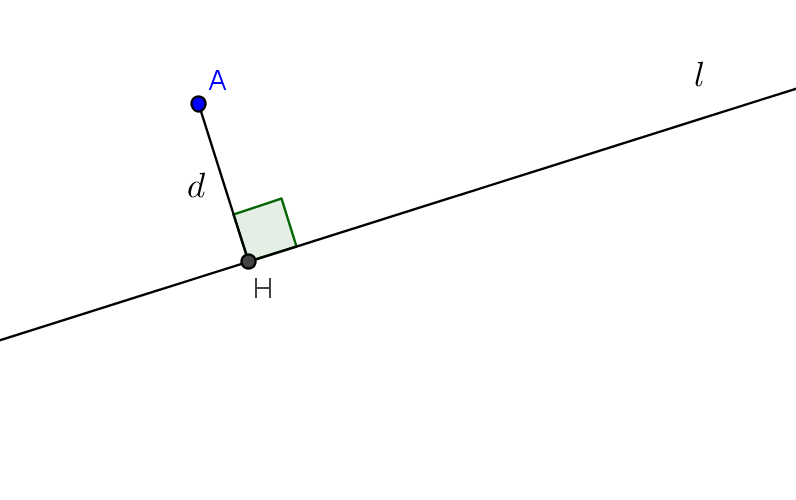
\includegraphics[width=0.5\textwidth]{line-point}
\caption{점과 직선 사이의 거리}
\label{line-point}
\end{figure}

%
\exam{}
다음의 직선의 방정식을 좌표평면 위에 나타내어라.\\
(1) \(y=x-3\)\\
(2) \(x+3y-9=0\)\\
(3) \(2y+6=0\)\\
(4) \(x-7=0\)

\sol
(1)
기울기가 \(1\)이고 \(y\)절편이 \(-3\)이다.
기울기가 \(1\)이므로 \(x\)가 \(1\)만큼 증가할 때마다 \(y\)도 1만큼 증가한다.
그리고 \(y\)절편이 \(-3\)이므로 \((0,-3)\)을 지난다.
따라서 그림 \ref{y=x-3}과 같은 그래프가 그려진다.

\begin{figure}[h!]
\center
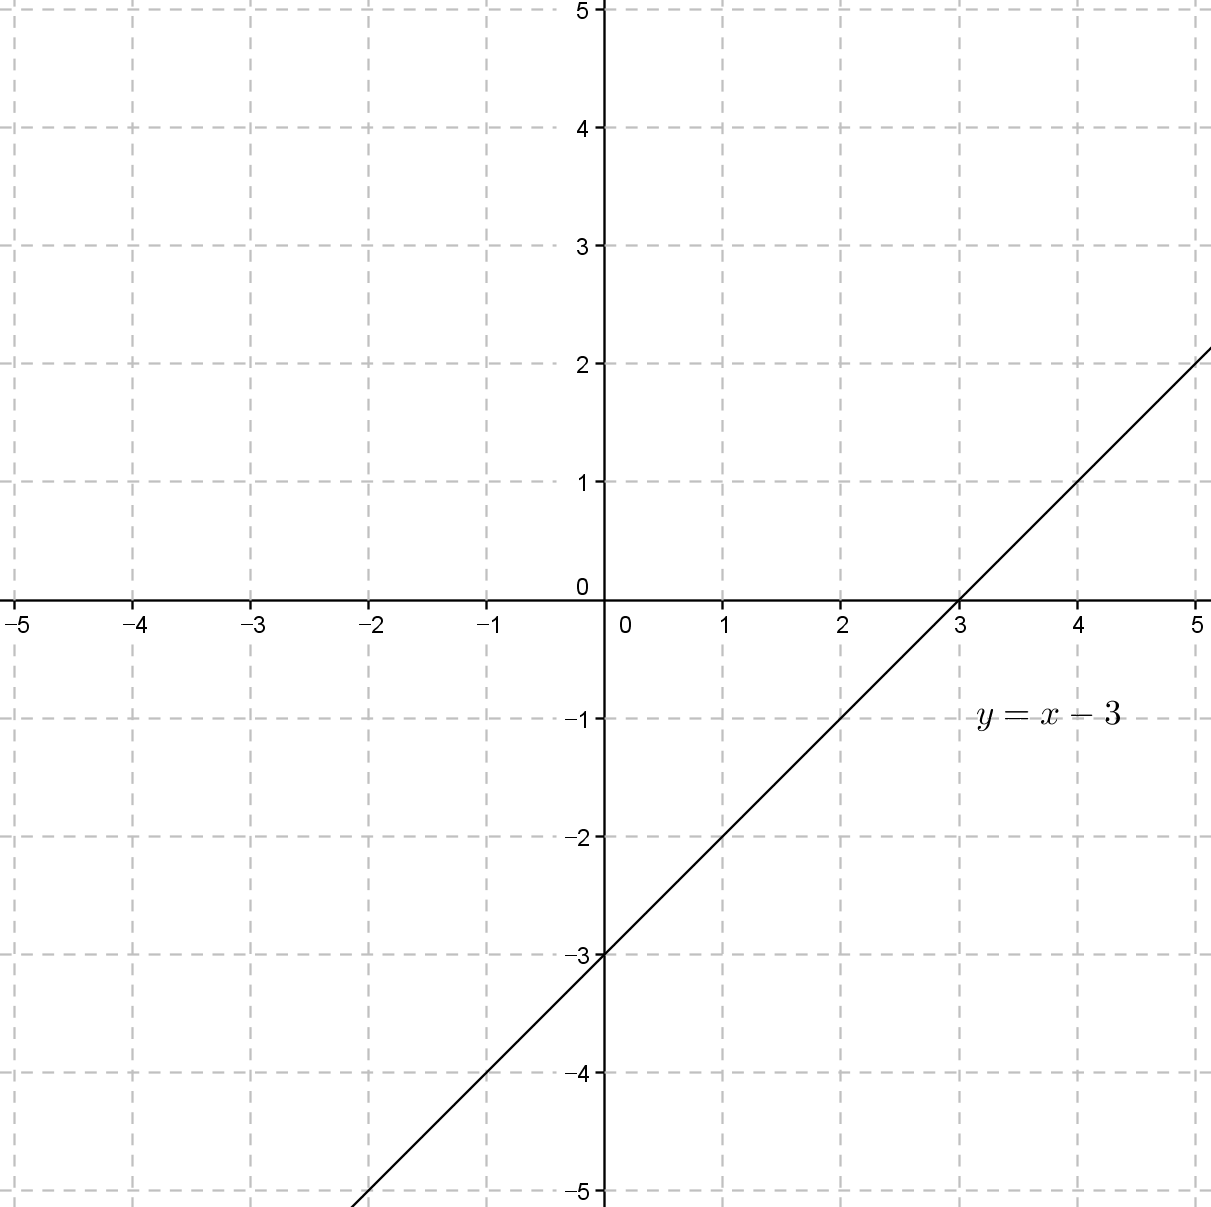
\includegraphics[width=0.4\textwidth]{y=x-3}
\caption{\(y=x-3\)의 그래프}
\label{y=x-3}
\end{figure}

(2)
주어진 식을 \(y=mx+n\)의 형태로 고치면 \(y=-\frac13x+3\)이 된다.
기울기가 \(-\frac13\)이므로 \(x\)가 \(3\)만큼 증가할 때마다 \(y\)는 \(1\)만큼 감소한다.
그리고 \(y\)절편이 \(3\)이므로 \((0,3)\)을 지난다.
따라서 그림 \ref{x+3y-9=0}과 같은 그래프가 그려진다.

\begin{figure}[h!]
\center
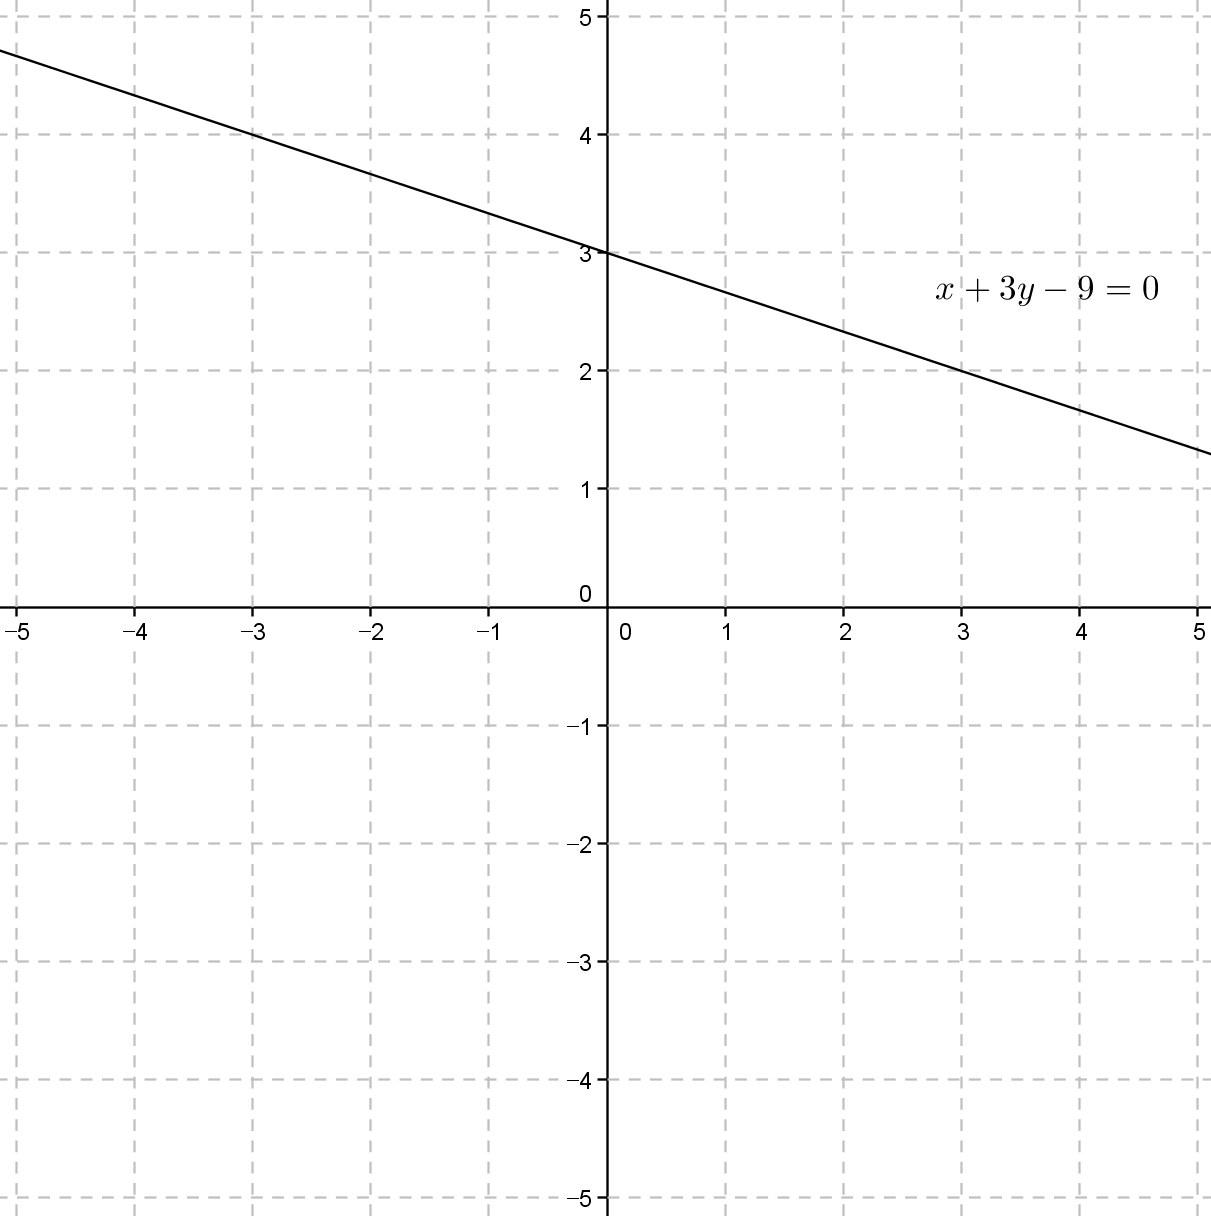
\includegraphics[width=0.4\textwidth]{x+3y-9=0}
\caption{\(x+3y-9=0\)의 그래프}
\label{x+3y-9=0}
\end{figure}

(3)
주어진 식을 변형하면 \(y=-3\)이 되고 이것은 \(y=0x-3\)이라고 생각할 수 있다.
기울기가 \(0\)이므로 \(x\)가 증가하더라도 \(y\)는 변화하지 않는다.
그리고 \(y\)절편이 \(-3\)이므로 \((0,-3)\)을 지난다.
따라서 그림 \ref{2y+6=0}과 같은 그래프가 그려진다.

사실, 주어진 식이 \(y=-3\)이므로 \(y\)좌표가 \(-3\)인 모든 점들을 찍어 표시하라는 의미이다.
그런 의미에서 그림 \ref{2y+6=0}에 그려진 직선은 잘 그려졌다고 볼 수 있다.

\begin{figure}[h!]
\center
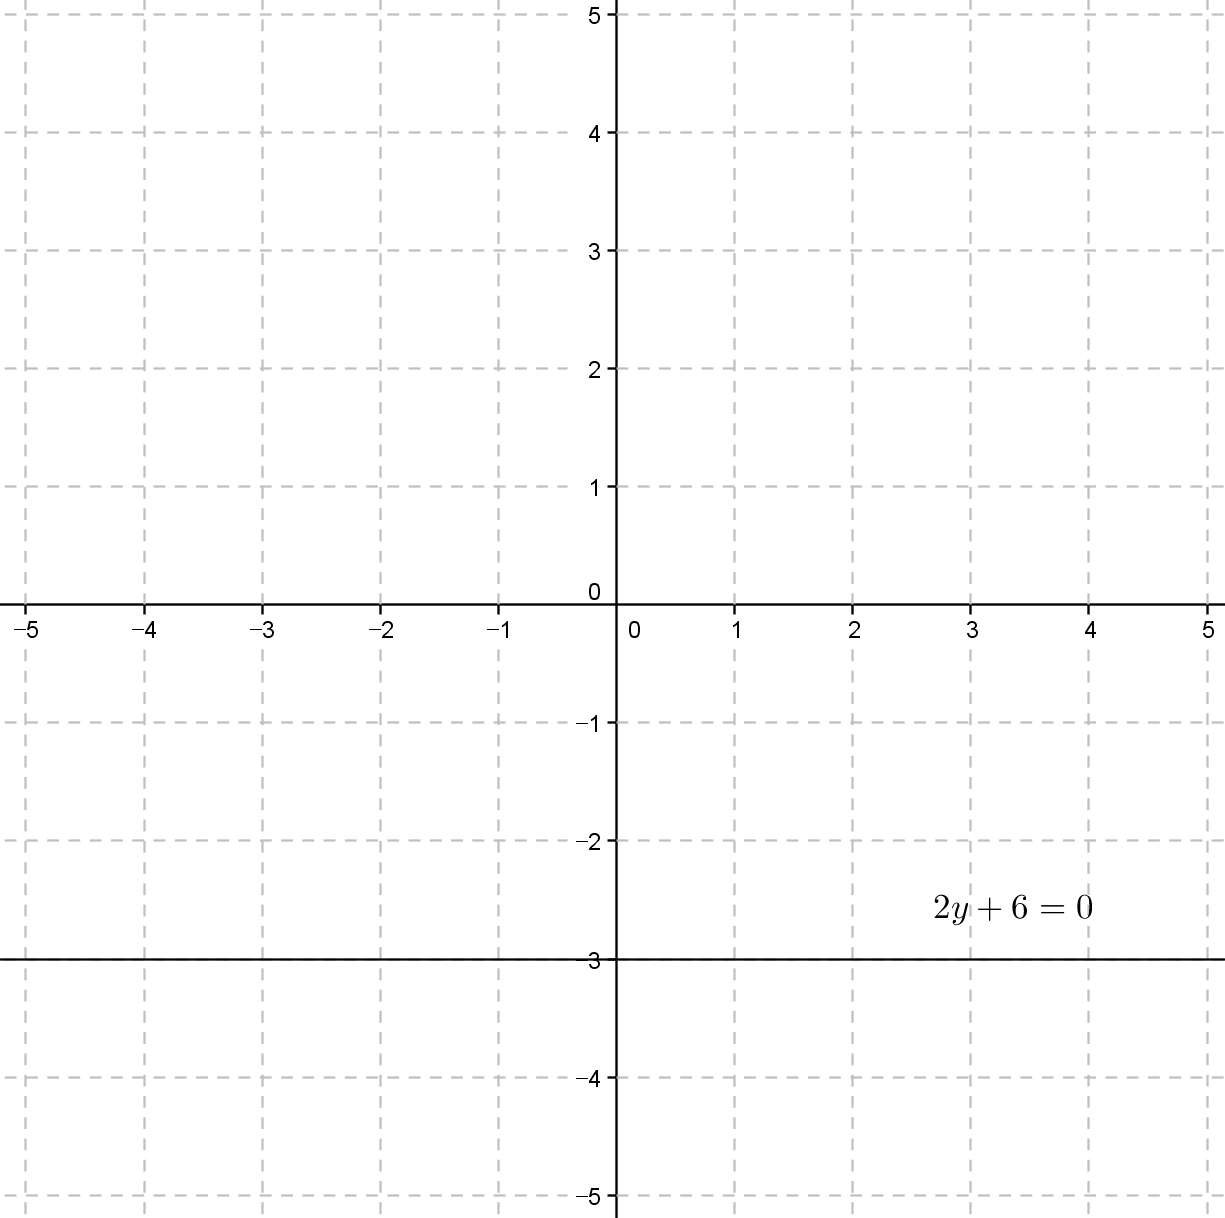
\includegraphics[width=0.4\textwidth]{2y+6=0}
\caption{\(2y+6=0\)의 그래프}
\label{2y+6=0}
\end{figure}

(4)
이번에는 주어진 식을 변형해 \(y=mx+n\)꼴로 나타내는 것이 불가능하다.
하지만 주어진 식이 \(x=7\)이므로 \(x\)좌표가 \(7\)인 모든 점들을 찍어 표시하라는 의미이다.
따라서 그림 \ref{x-7=0}과 같이 그래프가 그려진다.

\begin{figure}[h!]
\center
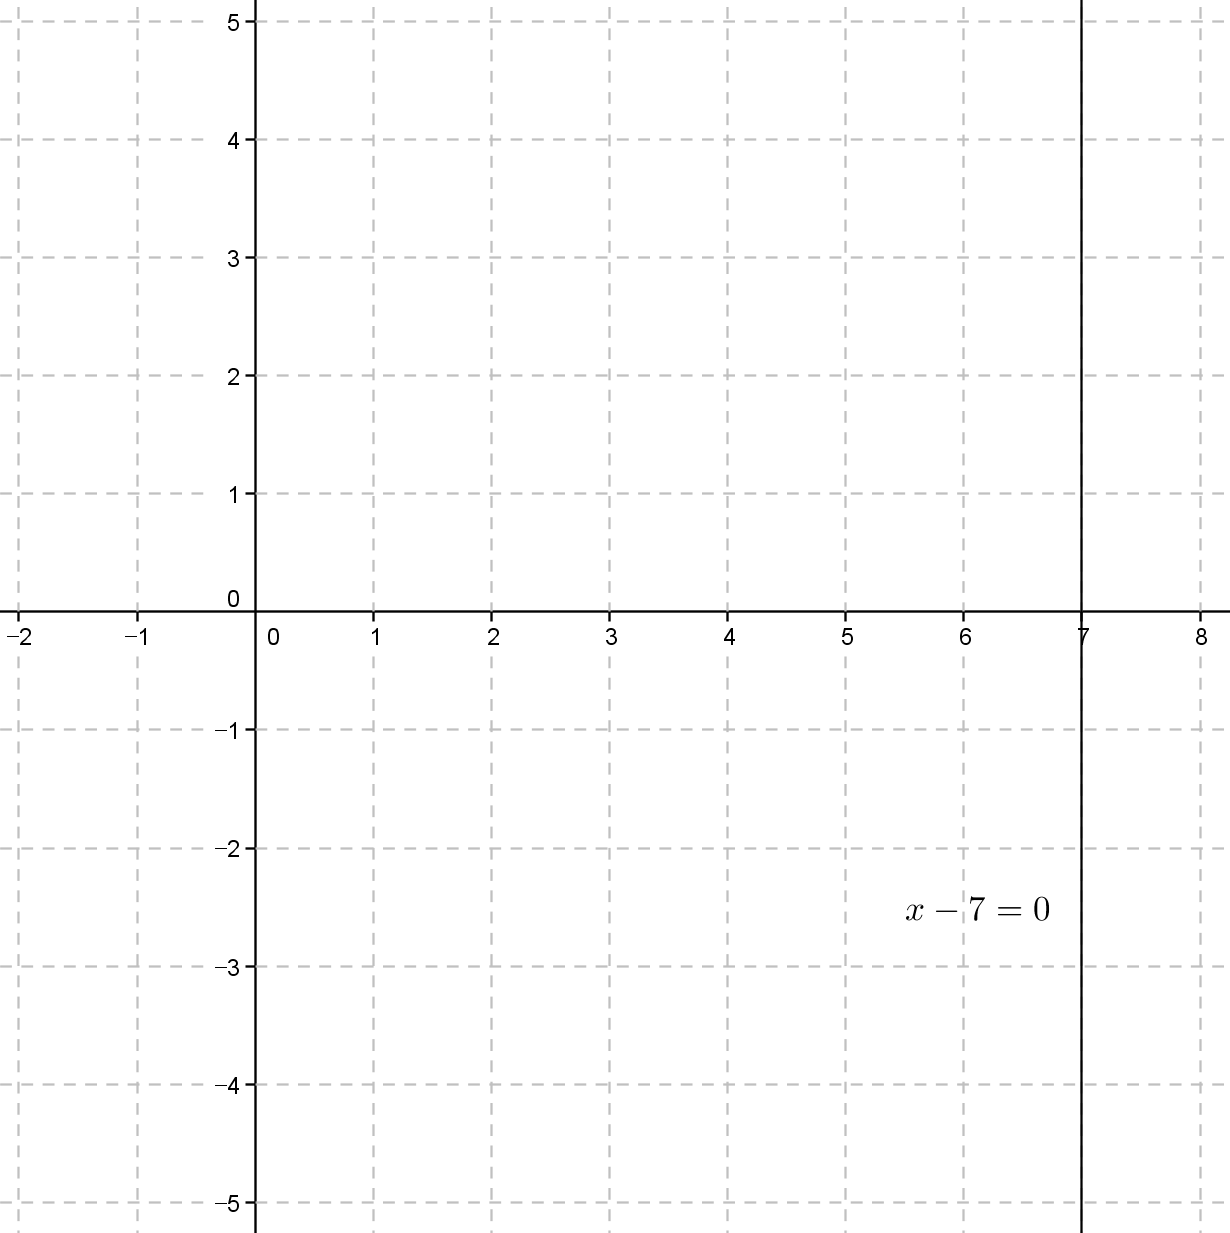
\includegraphics[width=0.4\textwidth]{x-7=0}
\caption{\(x-7=0\)의 그래프}
\label{x-7=0}
\end{figure}

%
\prob{}
다음 직선의 방정식을 좌표평면 위에 나타내어라.\\
(1) \(y=2x+1\)\\
(2) \(y=-3x\)\\
(3) \(y=\frac12x+\frac12\)\\
(4) \(y=-\frac32x+2\)\\
(5) \(x+y+1=0\)\\
(6) \(2x-4y-8=0\)\\
(7) \(3x-5=0\)\\
(8) \(2y-2=0\)

\ans{생략}

%
\exam{}
점 \((4,1)\)을 지나고 기울기가 \(3\)인 직선의 방정식을 구하여라.

\sol
공식
\[y-y_1=m(x-x_1)\]
에 \(m=3\), \((x_1,y_1)=(4,1)\)을 대입하면 \(y-1=3(x-4)\)이다.
이것을 정리하면 \(y=3x-11\)이 된다.
그래프를 그리면 그림 \ref{y=3x-11}과 같이 나타나며, 점 \((4,1)\)을 지나는 것을 확인할 수 있다.

\begin{figure}[h!]
\center
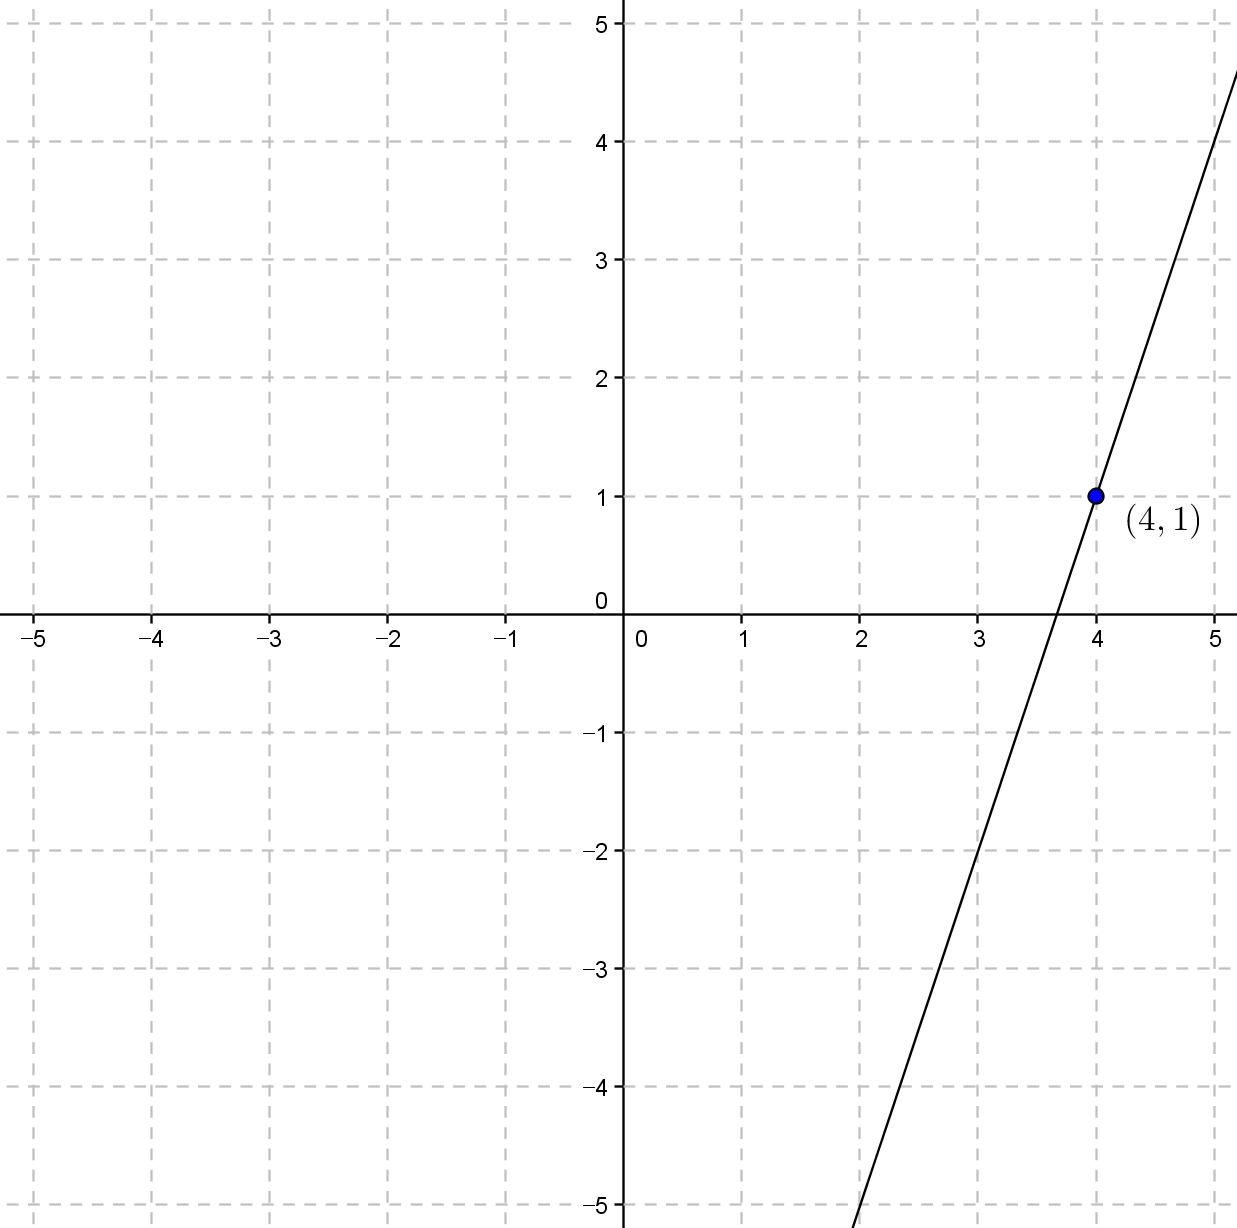
\includegraphics[width=0.4\textwidth]{y=3x-11}
\caption{기울기가 \(3\)이고 \((4,1)\)을 지나는 직선}
\label{y=3x-11}
\end{figure}

%
\prob{}
다음 직선의 방정식을 구하여라.\\
(1) 원점을 지나고 기울기가 \(-2\)인 직선\\
(2) 점 \((3,5)\)를 지나고 기울기가 \(3\)인 직선\\
(3) \(x\)절편이 \(-4\)이고 기울기가 \(2\)인 직선\\
(4) 점 \((-2,1)\)을 지나고 \(x\)축에 평행한 직선\\
(5) 점 \((5,-6)\)을 지나고 \(y\)축에 평행한 직선

\ans{
(1) \(y=-2x\) (2) \(y=3x-4\) (3) \(y=2x+8\) (4) \(y=1\) (5) \(x=5\)
}

%
\exam{}
다음 두 점을 지나는 직선의 방정식을 구하여라.\\
(1) \((3,-2)\), \((1,4)\)\\
(2) \((2,-3)\), \((2,5)\)

\sol
(1)
공식
\[y-y_1=\frac{y_2-y_1}{x_2-x_1}(x-x_1)\]
에 \((x_1,y_1)=(3,-2)\), \((x_2,y_2)=(1,4)\)를 대입하면 \(y-(-2)=\frac{4-(-2)}{1-3}(x-3)\)이다.
따라서 \(y+2=-3(x-3)\)이고 \(y=-3x+7\)이다(그림 \ref{y=-3x+7}).

\begin{figure}[h!]
\center
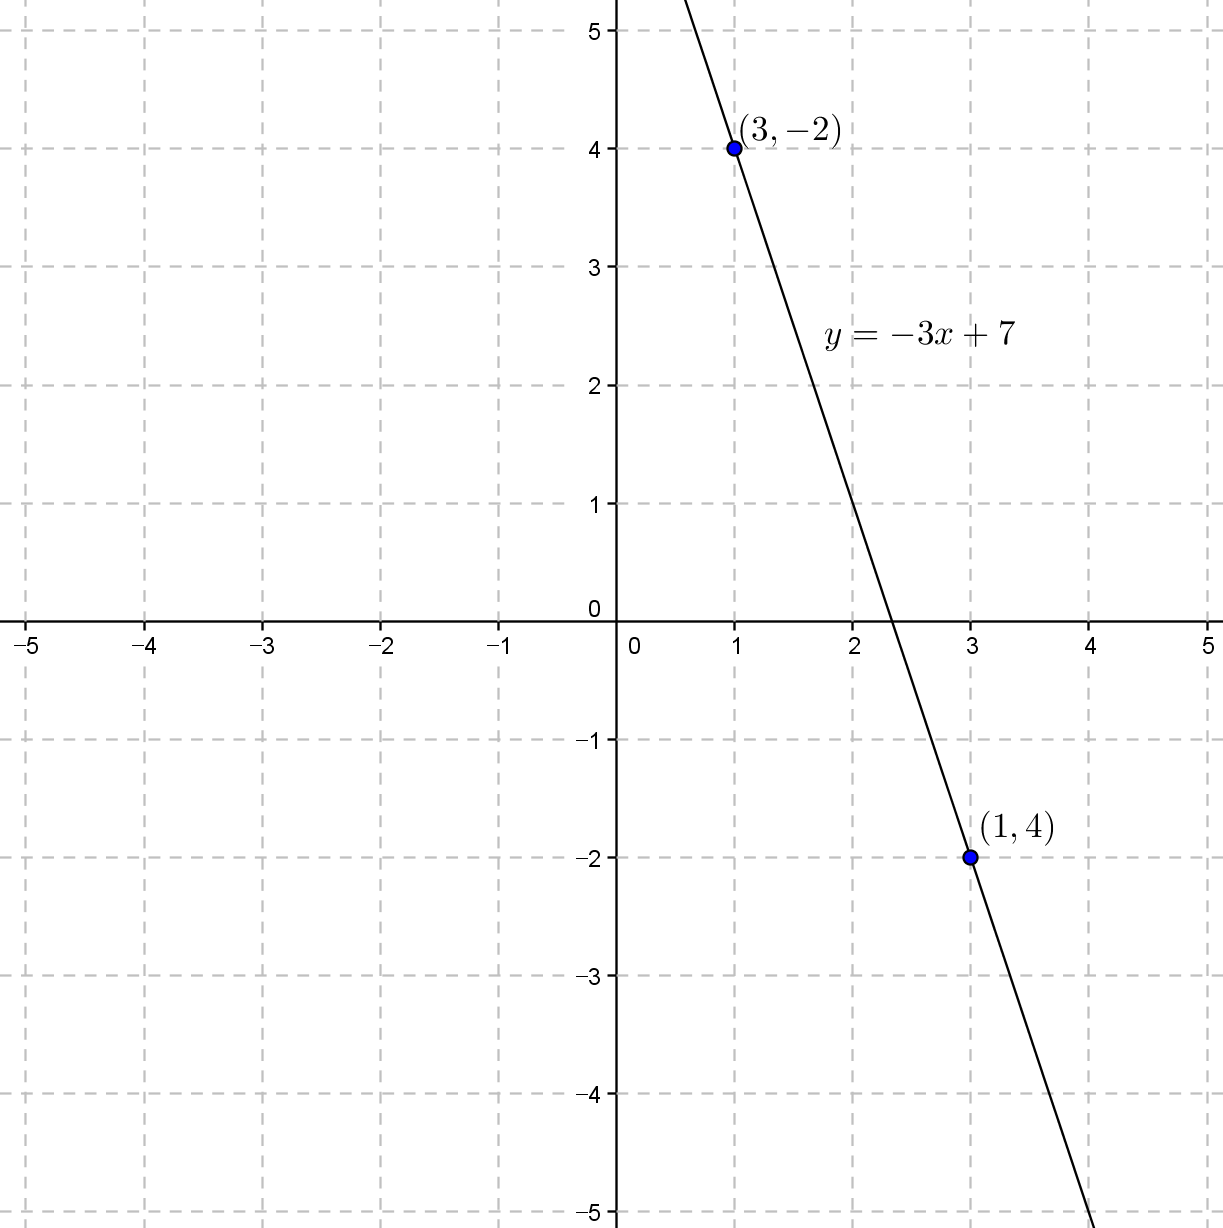
\includegraphics[width=0.4\textwidth]{y=-3x+7}
\caption{\((3,-2)\), \((1,4)\)를 지나는 직선}
\label{y=-3x+7}
\end{figure}

(2)
이 경우에는 (1)번에서 사용한 공식을 쓸 수 없다.
\(x_1=2\), \(x_2=2\)이므로 기울기의 분모가 0이 되기 때문이다.
하지만 좌표평면에 두 점을 찍고 두 점을 지나는 직선을 생각해보면 이 직선은 \(x=2\)가 되어야 함을 쉽게 알 수 있다(그림 \ref{x=2}).

\begin{figure}[h!]
\center
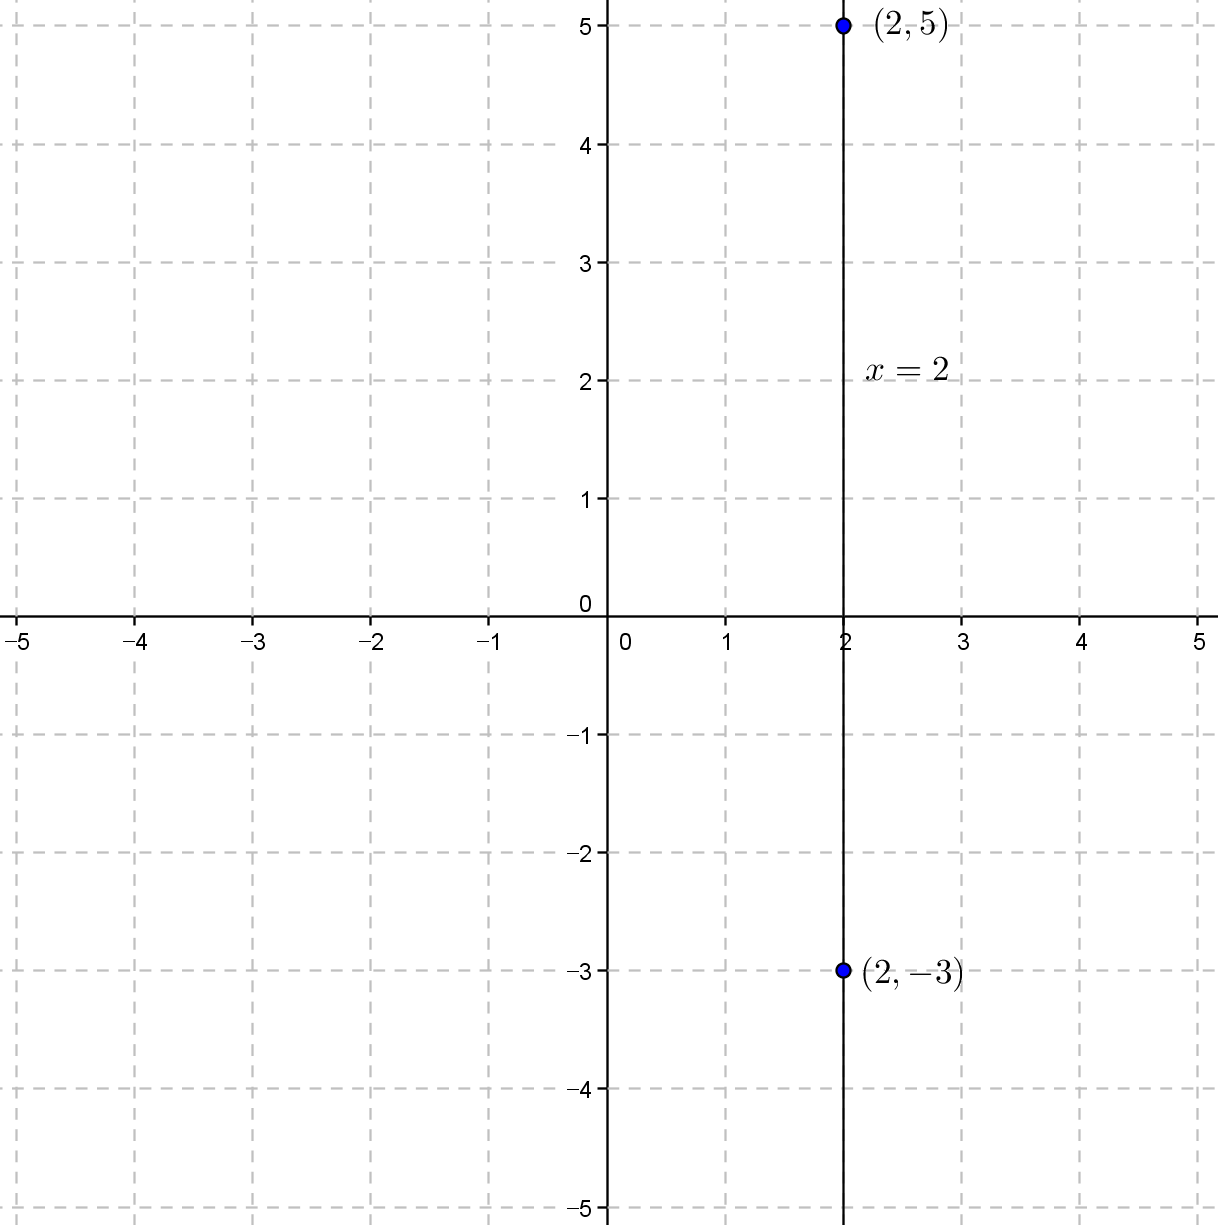
\includegraphics[width=0.4\textwidth]{x=2}
\caption{\((2,-3)\), \((2,5)\)를 지나는 직선}
\label{x=2}
\end{figure}

%
\prob{}
다음 두 점을 지나는 직선의 방정식을 구하여라.\\
(1) \((-1,6)\), \((3,2)\)\\
(2) \((0,-3)\), \((2,0)\)\\
(3) \((4,-1)\), \((3,-1)\)\\
(4) \((-2,5)\), \((-2,4)\)

\ans{
(1) \(y=-x+5\) (2) \(y=\frac32x-3\) (3) \(y=-1\) (4) \(x=-2\)}

%
\exam{}
다음 직선의 방정식을 구하여라.\\
(1) \((4,2)\)를 지나고 직선 \(y=2x-3\)에 평행한 직선\\
(2) \((3,-2)\)를 지나고 직선 \(3x-y+2=0\)에 수직인 직선

\sol
(1) 주어진 직선의 기울기가 \(2\)이므로 새로 구하려는 직선의 기울기도 \(2\)이다.
기울기가 \(2\)이고 \((4,2)\)를 지나는 직선이므로 \(y-2=2(x-4)\)이다.
이를 정리하면 \(y=2x-6\)이 된다(그림 \ref{y=2x-6}).

\begin{figure}[h!]
\center
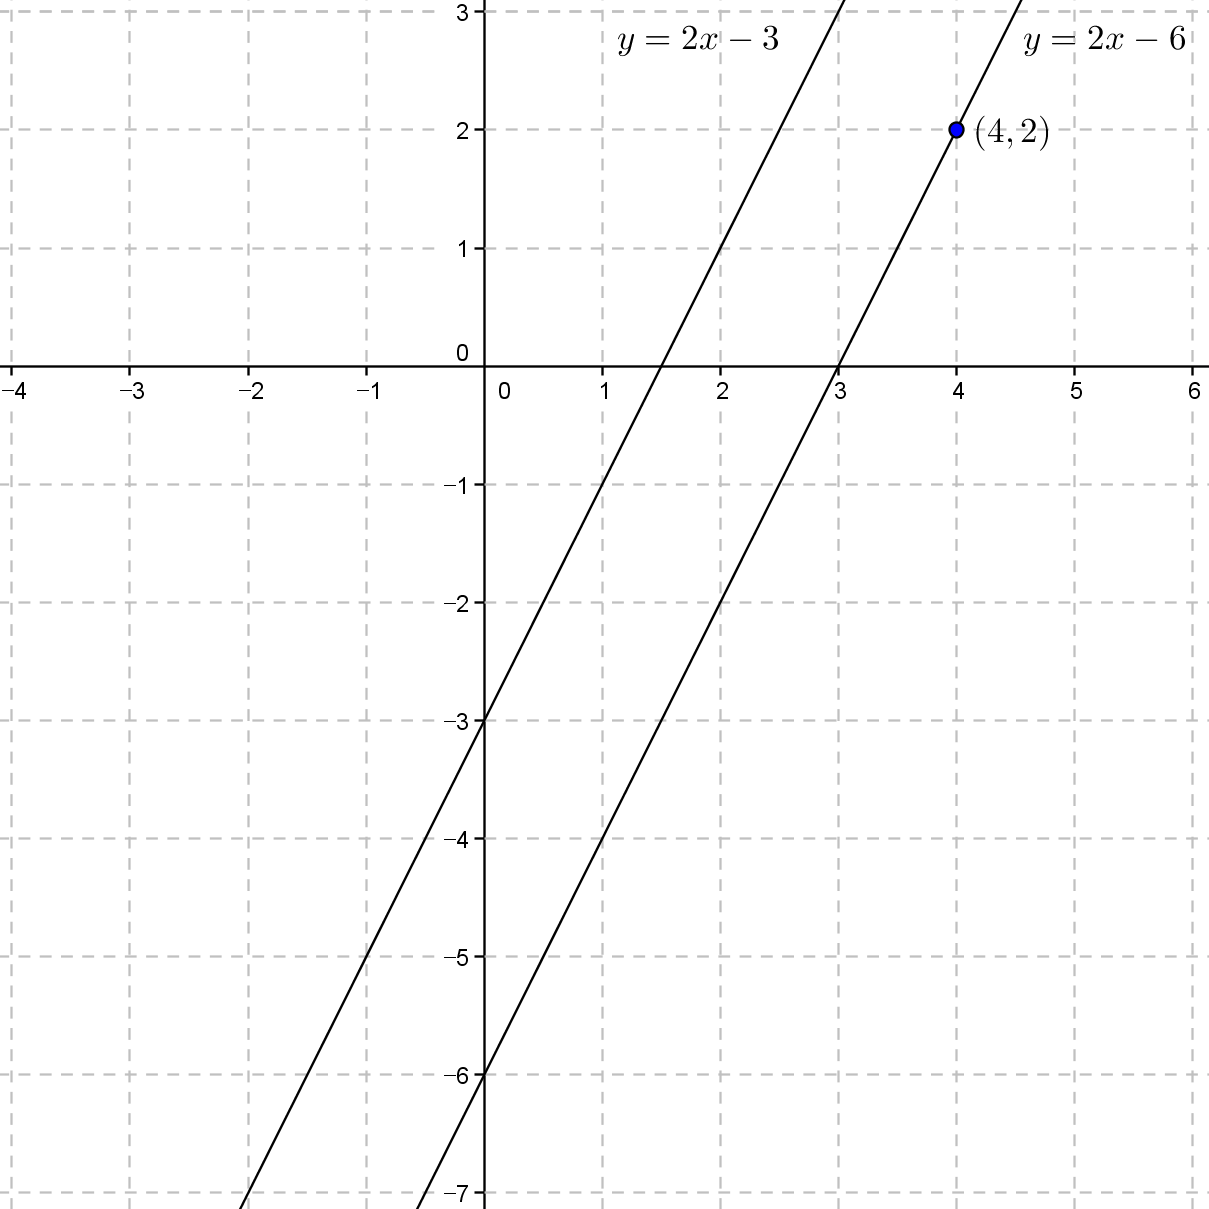
\includegraphics[width=0.4\textwidth]{y=2x-6}
\caption{\(y=2x-3\)에 평행하고 \((4,2)\)를 지나는 직선}
\label{y=2x-6}
\end{figure}

(2) 주어진 식을 정리하면 \(y=3x+2\)가 되므로 주어진 직선의 기울기는 \(3\)이다.
새로 구하려는 직선의 기울기를 \(m\)이라고 하면 \(3\times m=-1\)이므로 \(m=-\frac13\)이다.
(주어진 직선의 기울기인 \(3\)에 역수를 취해 \(\frac13\)을 만들고, 다시 \(\frac13\)에 마이너스를 붙인 \(-\frac13\)이 새로 구할 직선의 기울기라고 해도 된다.)
기울기가 \(-\frac13\)이고 \((3,-2)\)를 지나는 직선이므로 \(y+2=-\frac13(x-3)\)이다.
이를 정리하면 \(y=-\frac13x-1\)이 된다(그림 \ref{x+3y+3=0}).

\begin{figure}[h!]
\center
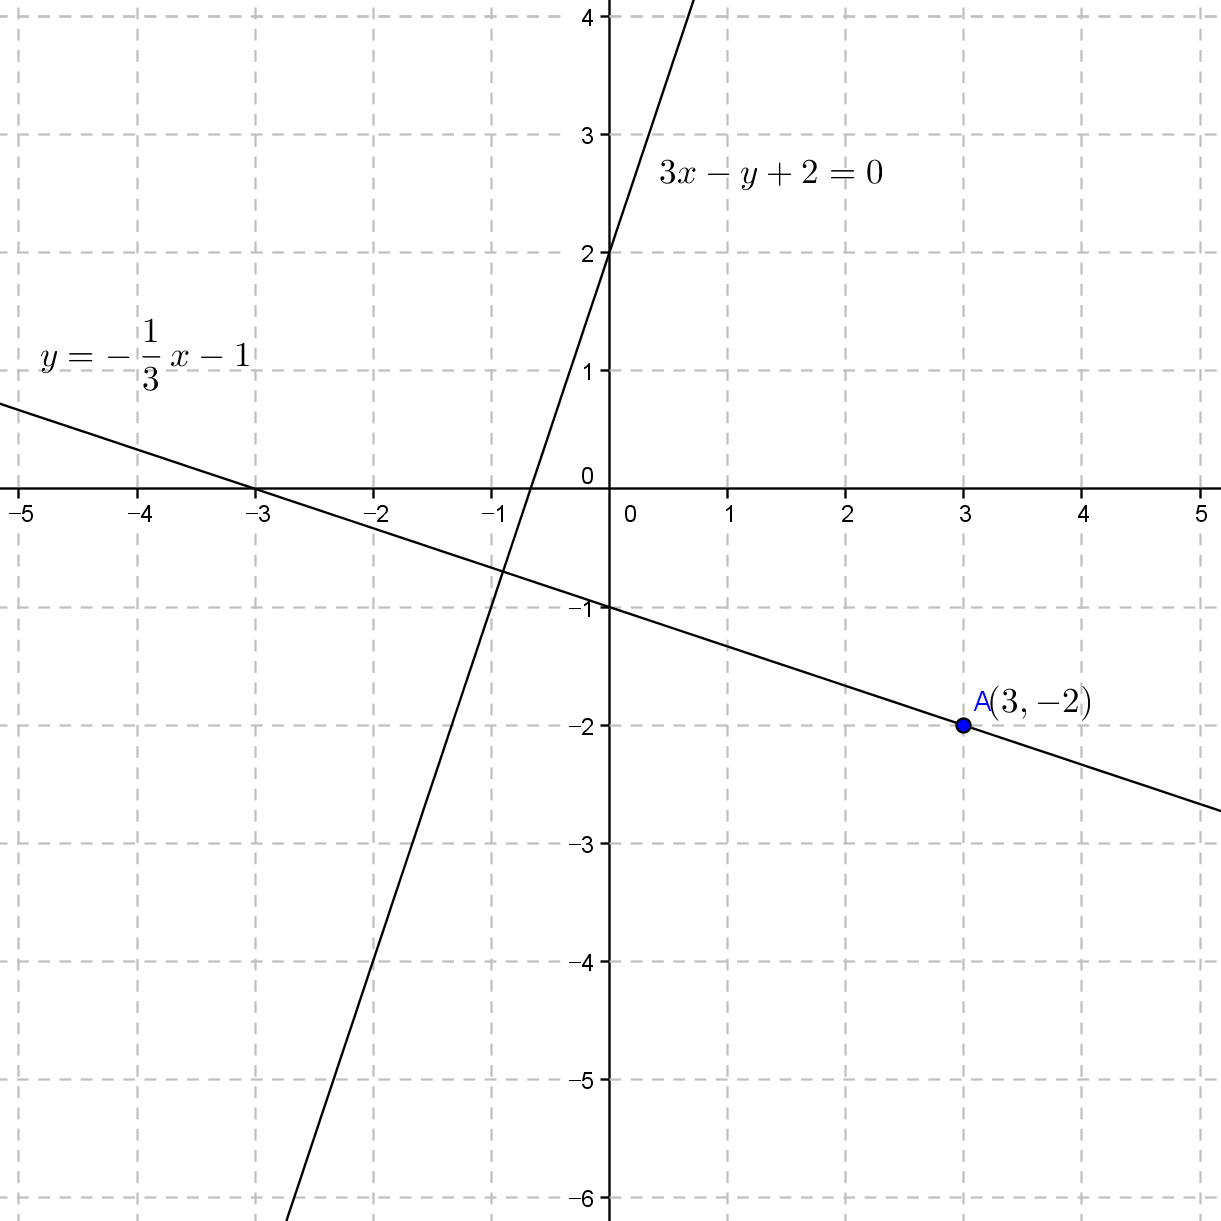
\includegraphics[width=0.4\textwidth]{x+3y+3=0}
\caption{\(3x-y+2=0\)에 수직하고 \((3,-2)\)를 지나는 직선}
\label{x+3y+3=0}
\end{figure}

%
\prob{}
점 \((3,-4)\)를 지나고 다음 직선에 평행한 직선의 방정식을 구하여라.\\
(1) \(y=2x-1\)\\
(2) \(2x+3y=5\)\\
(3) \(y-3=0\)\\
(4) \(x+5=0\)

\ans{
(1) \(y=2x-10\) (2) \(y=-\frac23x-2\) (3) \(y=-4\) (4) \(x=3\)}

%
\prob{}
점 \((1,-4)\)를 지나고 다음 직선에 수직인 직선의 방정식을 구하여라.\\
(1) \(y=5x-3\)\\
(2) \(x+3y-2=0\)

\ans{
(1) \(y=-\frac15x-\frac{19}5\) (2) \(y=3x-7\)}

%
\exam{}
두 직선 \(x-y+2=0\)과 \(3x+y-6=0\) 사이의 교점을 구하여라.

\sol
두 식을 변형하면 \(x-y=-2\), \(3x+y=6\)이다.
두 식을 서로 더하면 \(4x=4\)이고 따라서 \(x=1\)이다.
\(x=1\)을 첫번째 식에 대입하면 \(1-y+2=0\)이 되어 \(y=3\)이다.
따라서 \((1,3)\)이 구하려는 교점이다.

실제로 두 그래프를 그려보면 교점이 \((1,3)\)이라는 것을 알 수 있다(그림 \ref{intersect}).

\begin{figure}[h!]
\center
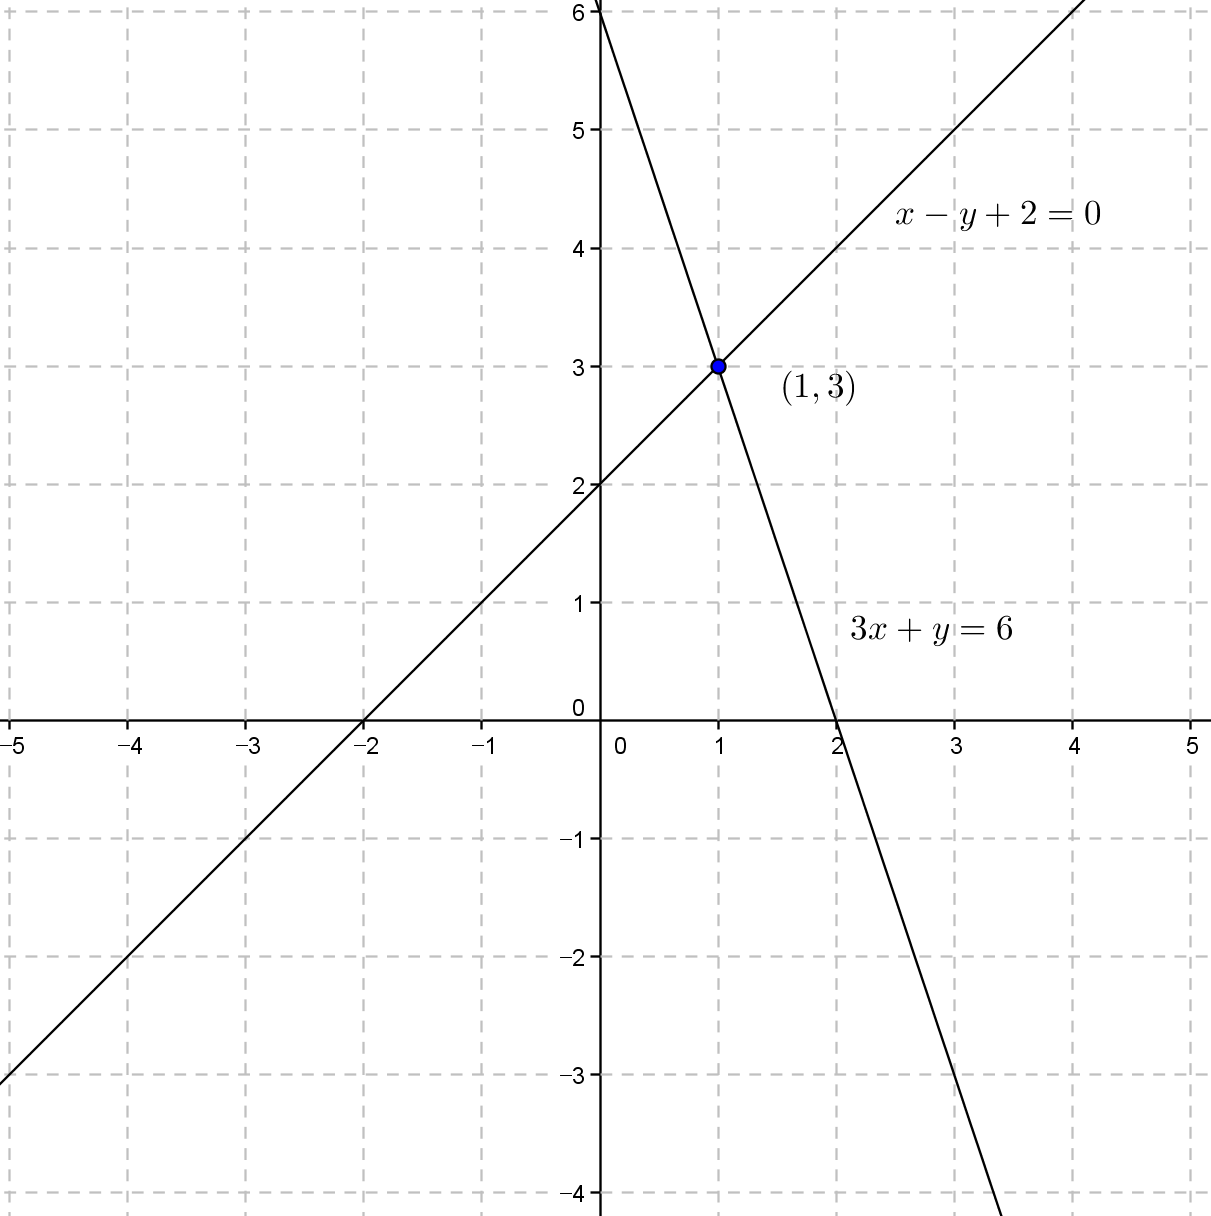
\includegraphics[width=0.4\textwidth]{intersect}
\caption{\(x-y+2=0\)과 \(3x+y-6=0\) 사이의 교점}
\label{intersect}
\end{figure}

%
\prob{}
두 직선 \(2x+y-3=0\), \(x-2y-4=0\)의 교점을 구하고, 이 교점과 점 \((3,0)\)을 지나는 직선의 방정식을 구하여라.

\ans{\(x-y-3=0\)}

%
\exam{}
다음 점과 직선 사이의 거리를 구하여라.\\
(1) 점 \((-2,1)\), 직선 \(3x+4y+12=0\)\\
(2) 원점, 직선 \(y=x+1\)

\sol
(1)
공식 \(d=\frac{|ax_1+by_1+c|}{\sqrt{a^2+b^2}}\)에 \(a=3\), \(b=4\), \(c=12\), \((x_1,y_1)=(-2,1)\)을 대입하면
\[
d=\frac{|3\times(-2)+4\times1+12|}{\sqrt{3^2+4^2}}=\frac{|10|}{\sqrt{25}}=\frac{10}5=2
\]
이다(그림 \ref{3x+4y+12=0}).

\begin{figure}[h!]
\center
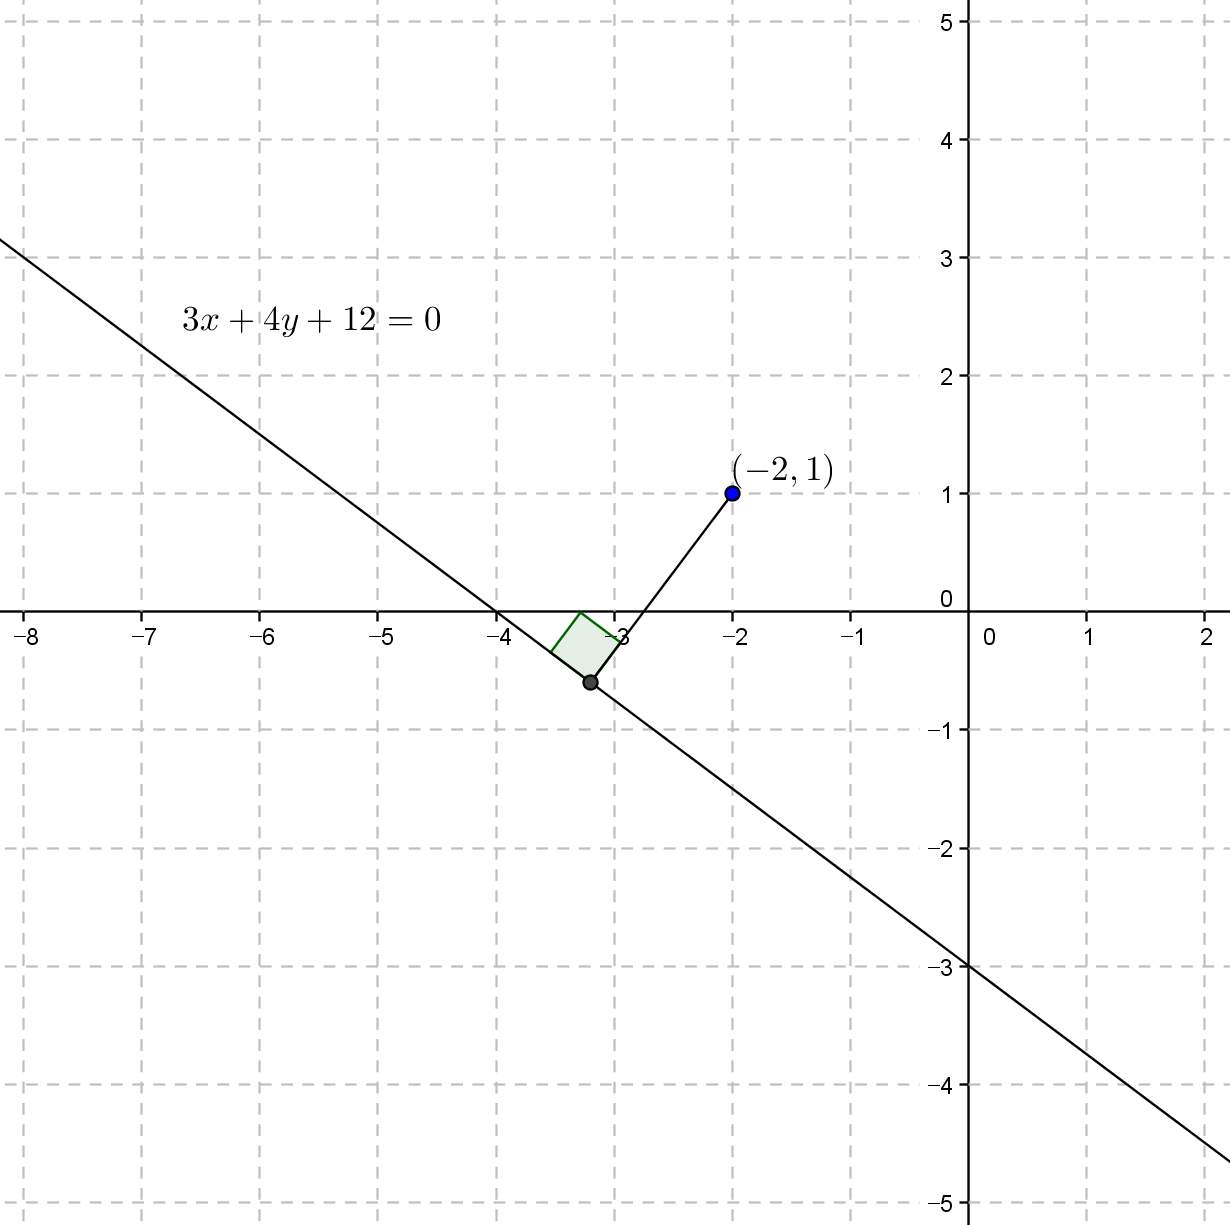
\includegraphics[width=0.4\textwidth]{3x+4y+12=0}
\caption{\((-2,1)\)에서 \(3x+4y+12=0\)까지의 거리}
\label{3x+4y+12=0}
\end{figure}

(2)
공식에 대입하기 전에 주어진 직선을 \(ax+by+c=0\)꼴로 고치면 \(x-y+1=0\)이므로 \(a=1\), \(b=-1\), \(c=1\)이다.
또 \((x_1,y_1)=(0,0)\)이므로
\[
d=\frac{|1\times0+(-1)\times0+1|}{\sqrt{1^2+(-1)^2}}=\frac{|1|}{\sqrt2}=\frac1{\sqrt2}
\]
이다(그림 \ref{y=x+1}).

\begin{figure}[h!]
\center
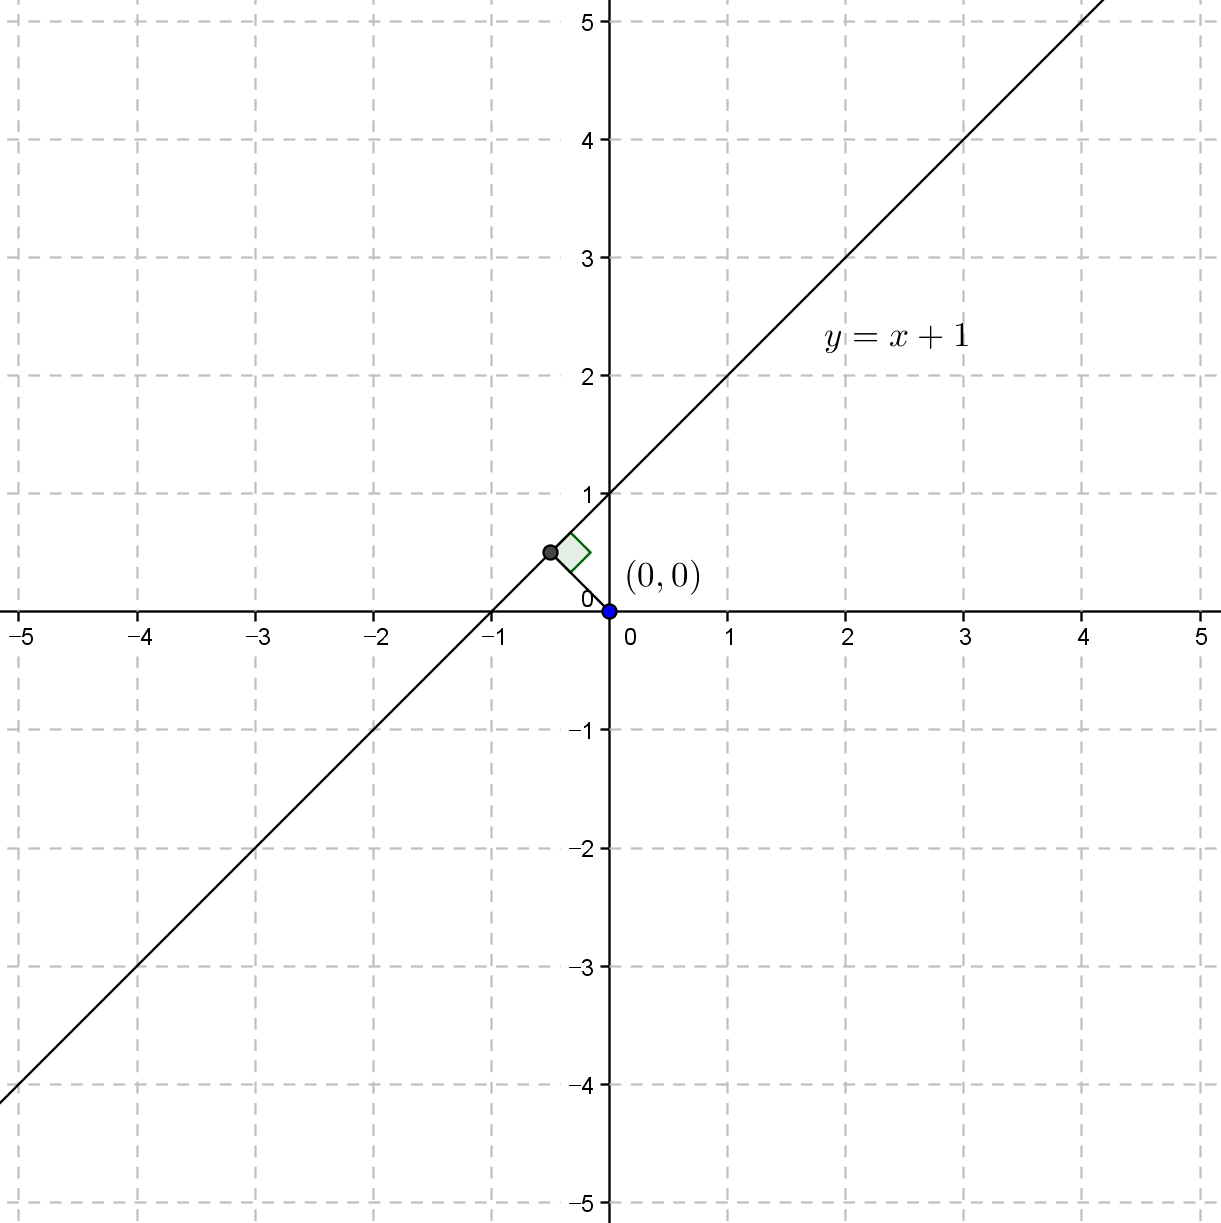
\includegraphics[width=0.4\textwidth]{y=x+1}
\caption{\((0,0)\)에서 \(y=x+1\)까지의 거리}
\label{y=x+1}
\end{figure}

%
\prob{}
다음 점과 직선 사이의 거리를 구하여라.\\
(1) 점 \((4,1)\), 직선 \(5x-12y-2=0\)\\
(2) 원점, 직선 \(2x-3y+13=0\)

\ans{
(1) \(\frac6{13}\) (2) \(\sqrt{13}\)
}

\exam{}
직선 \(3x+4y+1=0\)에 평행하고 점 \((3,-2)\)까지의 거리가 \(2\)인 직선의 방정식을 구하여라.

\sol
주어진 직선의 기울기가 \(-\frac34\)이므로 새로 구할 직선의 방정식도 \(-\frac34\)이다.
따라서 새로 구할 직선의 방정식을 \(y=-\frac34x+k\)라고 놓자.
이 식을 변형하면 \(3x+4y-4k=0\)이 된다.
이제 주어진 조건을 사용하면(\(a=3\), \(b=4\), \(c=-4k\), \((x_1,y_1)=(3,-2)\))
\[
2=d=\frac{|ax_1+by_1+c|}{\sqrt{a^2+b^2}}=\frac{|3\times3+4\times(-2)-4k|}{\sqrt{25}}=\frac{|1-4k|}5
\]
이다.
따라서 \(|1-4k|=10\)이고 \(1-4k=\pm10\)이다.

\(1-4k=10\)이면 \(k=-\frac94\)이고 이 때의 답은 \(y=-\frac34x-\frac94\)이다.

\(1-4k=-10\)이면 \(k=\frac{11}4\)이다 이 때의 답은 \(y=-\frac34x+\frac{11}4\)이다.

%
\prob{}
직선 \(y=2x+1\)에 평행하고 원점까지의 거리가 \(\frac{2}{\sqrt5}\)인 직선의 방정식을 구하여라.

\ans{\(y=2x+2\) 또는 \(y=2x-2\)}

%
\exam{}
원점과 직선 \(x+y+c=0\) 사이의 거리가 \(\sqrt2\)일 때, 실수 \(c\)의 값을 구하여라.

\sol
공식에 그대로 대입하면
\[\sqrt2=d=\frac{1\times0+1\times0+c|}{\sqrt{1^2+1^2}}=\frac{|c|}{\sqrt2}\]
이므로 \(|c|=2\)이다.
따라서 \(c=\pm2\)이다.
%
%\(c=2\)이면 답은 \(x+y+2=0\)이고
%\(c=-2\)이면 답은 \(x+y-2=0\)이다.

%
\prob{}
점 \((-3,4)\)와 직선 \(y=mx-5\) 사이의 거리가 \(3\sqrt5\)일 때, 실수 \(m\)의 값을 구하여라.

\ans{\(m=-\frac12\) 또는 \(m=2\)}


%%
\section{원의 방정식(1)}

%
\summ{}
\begin{enumerate}
\item
중심이 \(C(a,b)\)이고 반지름이 \(r\)인 원의 방정식은 \((x-a)^2+(y-b)^2=r^2\)이다.
\end{enumerate}

%
\exam{}
방정식 \(x^2+y^2-2x-4y-11=0\)이 나타내는 원의 중심과 반지름의 길이를 구하여라.

\sol
\begin{gather*}
x^2+y^2-2x-4y-11=0\\
(x^2-2x+1)+(y^2-4y+4)-11-5=0\\
(x-1)^2+(y-2)^2=4^2
\end{gather*}
이므로 원의 중심은 \((1,2)\)이고 반지름의 길이는 \(4\)이다.

\prob{}
다음 방정식이 나타내는 원의 중심과 반지름의 길이를 구하여라.\\
(1) \(x^2+y^2-10x=0\)\\
(2) \(x^2+y^2+8x-2y+8=0\)\\
(3) \(x^2+y^2-6x+3=0\)\\
(4) \(x^2+y^2+4x+12y+36=0\)

\ans{
(1) 중심 : \((5,0)\), 반지름의 길이 : \(5\)\\
(2) 중심 : \((-4,1)\), 반지름의 길이 : \(3\)\\
(3) 중심 : \((3,0)\), 반지름의 길이 : \(\sqrt6\)\\
(4) 중심 : \((-2,-6)\), 반지름의 길이 : \(2\)
}

\exam{}
세 점 \(A(1,-1)\), \(B(0,6)\), \(C(2,2)\)를 지나는 원의 방정식을 구하여라.

\sol
구하는 원의 방정식을
\[x^2+y^2+Ax+By+C=0\]
이라고 놓으면 세 점이 원 위에 있다는 조건으로부터
\begin{align*}
1^2+(-1)^2+A-B+C	&=0\\
0^2+6^2+0+6B+C 	&=0\\
2^2+2^2+2A+2B+C 	&=0
\end{align*}
이다.
혹은
\begin{align}
A-B+C	&=-2\\
6B+C 	&=-36\\
2A+2B+C 	&=-8
\end{align}
이다.
\((3)-(1)\times2\)을 하면
\begin{equation}
4B-C=-4
\end{equation}
이 되고, 다시
\((2)+(4)\)를 하면
\[10B=-40\]
이므로 \(B=-4\)이다.
(2)에 대입하면 \(C=-12\)이고, 다시 (1)에 대입하면 \(A=6\)이다.

따라서 구하는 원의 방정식은
\[x^2+y^2+6x-4y-12=0\]
이다.
\bigskip

\textbf{*(다른 방식의 풀이)}\\
구하려는 원의 중심을 \(P(a,b)\)라고 놓으면 \(\overline{AP}=\overline{BP}=\overline{CP}\)가 성립해야 하므로 \(\overline{AP}^2=\overline{BP}^2\)으로부터
\begin{equation}
(a-1)^2+(b+1)^2=a^2+(b-6)^2
\end{equation}
을 얻고, \(\overline{BP}^2=\overline{CP}^2\)으로부터
\begin{equation}
a^2+(b-6)^2=(a-2)^2+(b-2)^2
\end{equation}
을 얻는다.
(5)번 식을 정리하면
\begin{equation}
2a-14b=-34
\end{equation}
이고, (6)번 식을 정리하면
\begin{equation}
4a-8b=-28
\end{equation}
이다.
이들을 더 정리하면
\begin{gather}
a-7b=-17\\
a-2b=-7
\end{gather}
이다.
\((10)-(9)\)에서
\[5b=10\]
이 되어 \(b=2\)이고, (10)에 다시 대입하면 \(a=-3\)이다.
즉 구하려는 원의 중심은 \((-3,2)\)이다.
한편 반지름의 길이는 \(\overline{AP}\)와 같은데
\[\overline{AP}=\sqrt{(-3-1)^2+(2+1)^2}=\sqrt{25}=5\]
이므로 반지름의 길이는 \(5\)이다.

따라서 구하는 원의 방정식은
\[(x+3)^2+(y-2)^2=25\]
이다.
이것은 아까 구한 원의 방정식과 정확히 일치한다(그림 \ref{x^2+y^2+6x-4y-12=0}).

\begin{figure}[h!]
\center
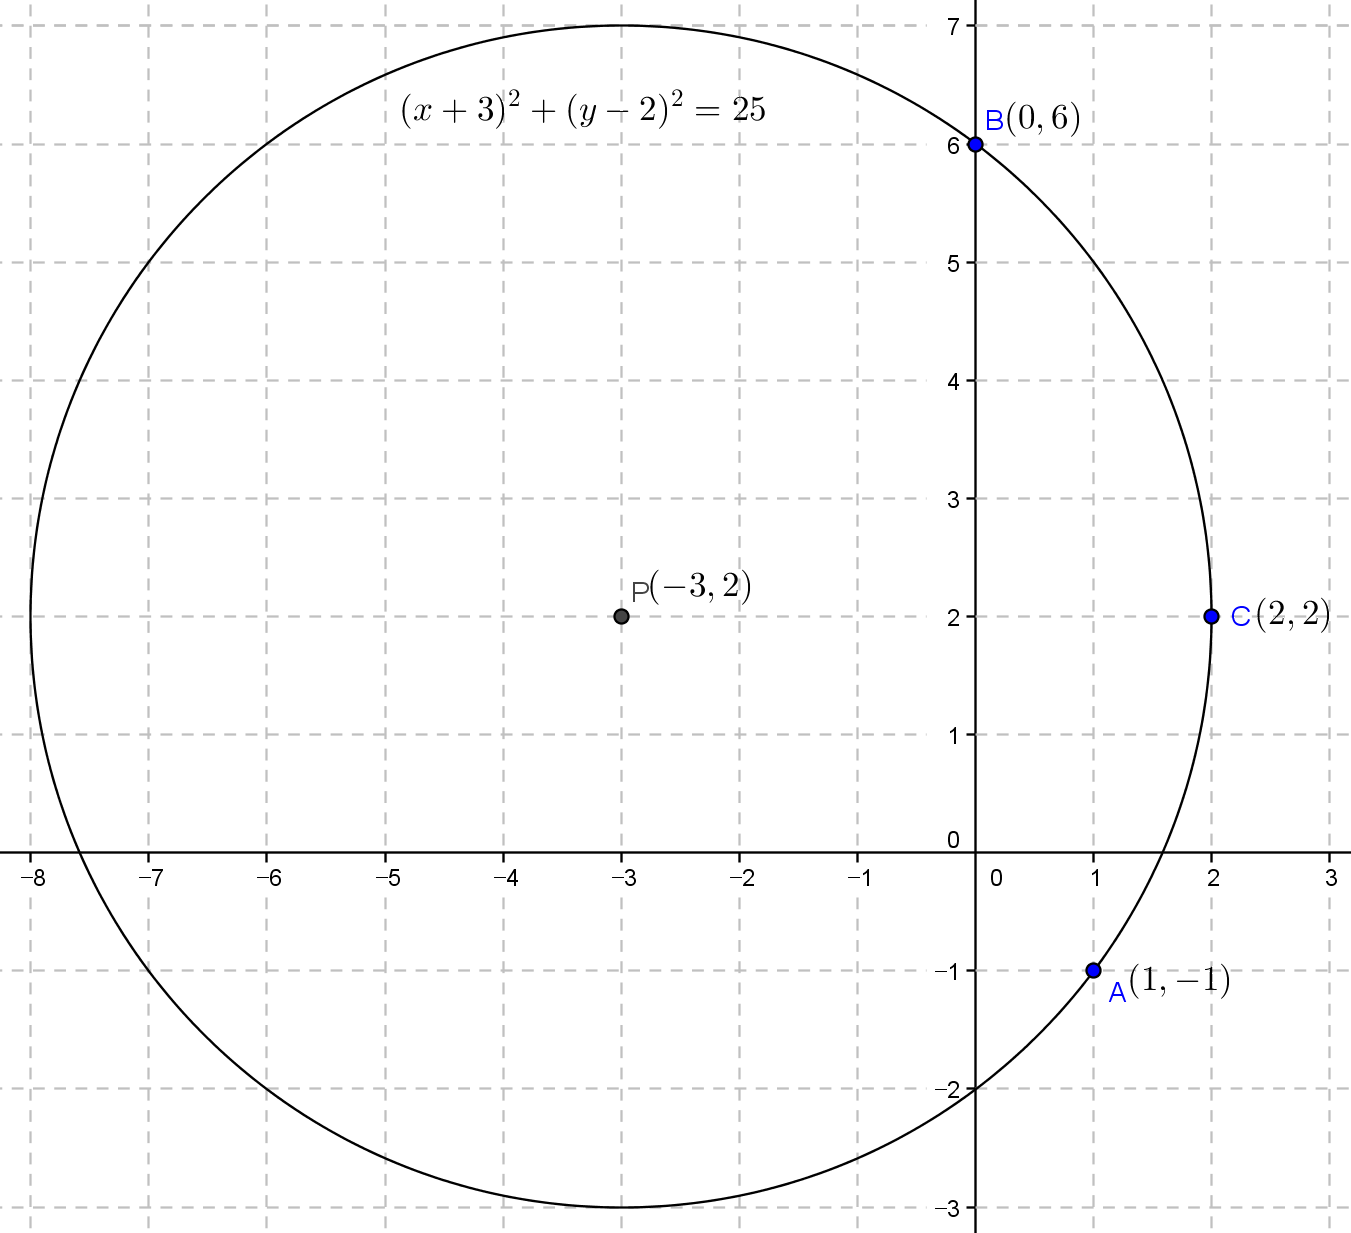
\includegraphics[width=0.4\textwidth]{x^2+y^2+6x-4y-12=0}
\caption{세 점 \(A(1,-1)\), \(B(0,6)\), \(C(2,2)\)를 지나는 원}
\label{x^2+y^2+6x-4y-12=0}
\end{figure}

\setcounter{equation}{0}

%
\prob{}
다음 세 점을 지나는 원의 방정식을 구하여라.\\
(1) \((0,0)\), \((0,2)\), \((1,3)\)\\
(2) \((-1,5)\), \((-5,3)\), \((2,-4)\)

\ans{
(1) \(x^2+y^2-4x-2y=0\)\\
(2) \(x^2+y^2+2x-24=0\)
}

%
\exam{아폴로니우스의 원}
두 점 \(A(-3,0)\), \(B(2,0)\)에 대하여 \(\overline{AP}:\overline{BP}=2:3\)인 점 \(P\)가 나타내는 도형을 구하여라.

\sol
점 \(P\)의 좌표를 \((x,y)\)라고 가정하고, 주어진 조건으로부터 \(x\)와 \(y\)사이의  관계식을 도출하자.

주어진 조건을 변형하면 \(3\overline{AP}=2\overline{BP}\)이고 양변을 제곱하면 \(9\overline{AP}^2=4\overline{BP}^2\)이다.
따라서
\[9[(x+3)^2+y^2]=4[(x-2)^2+y^2]\]
이다.
양변을 전개한 후 모든 항을 좌변으로 이항시키면
\[5x^2+5y^2+70x+65=0\]
다시 양변을 \(5\)로 나누면
\[x^2+y^2+14x+13=0\]
이다.
이것이 점 \(P\)가 나타내는 도형이다.
조금 더 정리하면
\[(x+7)^2+y^2=36\]
이다.
즉 원의 중심이 \((-7,0)\)에 있고, 반지름의 길이가 \(6\)인 원이다.

\textbf{*(다른 방식의 풀이)}\\
선분 \(AB\)에서 \(\overline{AC}:\overline{BC}=2:3\)인 내분점을 \(C\)라고 하고, \(\overline{AD}:\overline{BD}=2:3\)인 외분점을 \(D\)라고 하자.
그러면
\begin{align*}
C&=\left(\frac{2\times2+3\times(-3)}{2+3},\frac{2\times0+3\times0}{2+3}\right)=\left(-1,0\right)\\
D&=\left(\frac{2\times2-3\times(-3)}{2-3},\frac{2\times0-3\times0}{2-3}\right)=\left(-13,0\right)
\end{align*}
이고, 이 두 점은 우리가 구하려는 도형 위의 점들이다.

평면 상에서 고정된 두 점으로부터의 길이의 비가 일정한 점이 그리는 도형이 원이라는 사실은 알려져있다.
따라서 우리가 구하려는 원은 두 점 \(C\), \(D\)를 지나는 원이다.
또한 구하려는 원은 직선 \(AB\)에 대해 대칭일 것이므로 \(C\)와 \(D\)는 지름의 양 끝점이어야 한다.
따라서 원의 중심은 \(C\)와 \(D\)의 중점인
\[M=\left(\frac{-1-13}2,\frac{0+0}2\right)=(-7,0)\]
이고, 반지름은 \(\overline{CM}=6\)이어야 한다.
그러므로 \(P\)가 그리는 도형은
\[(x+7)^2+y^2=36\]
이다(그림 \ref{appolonius}).

\begin{figure}[h!]
\center
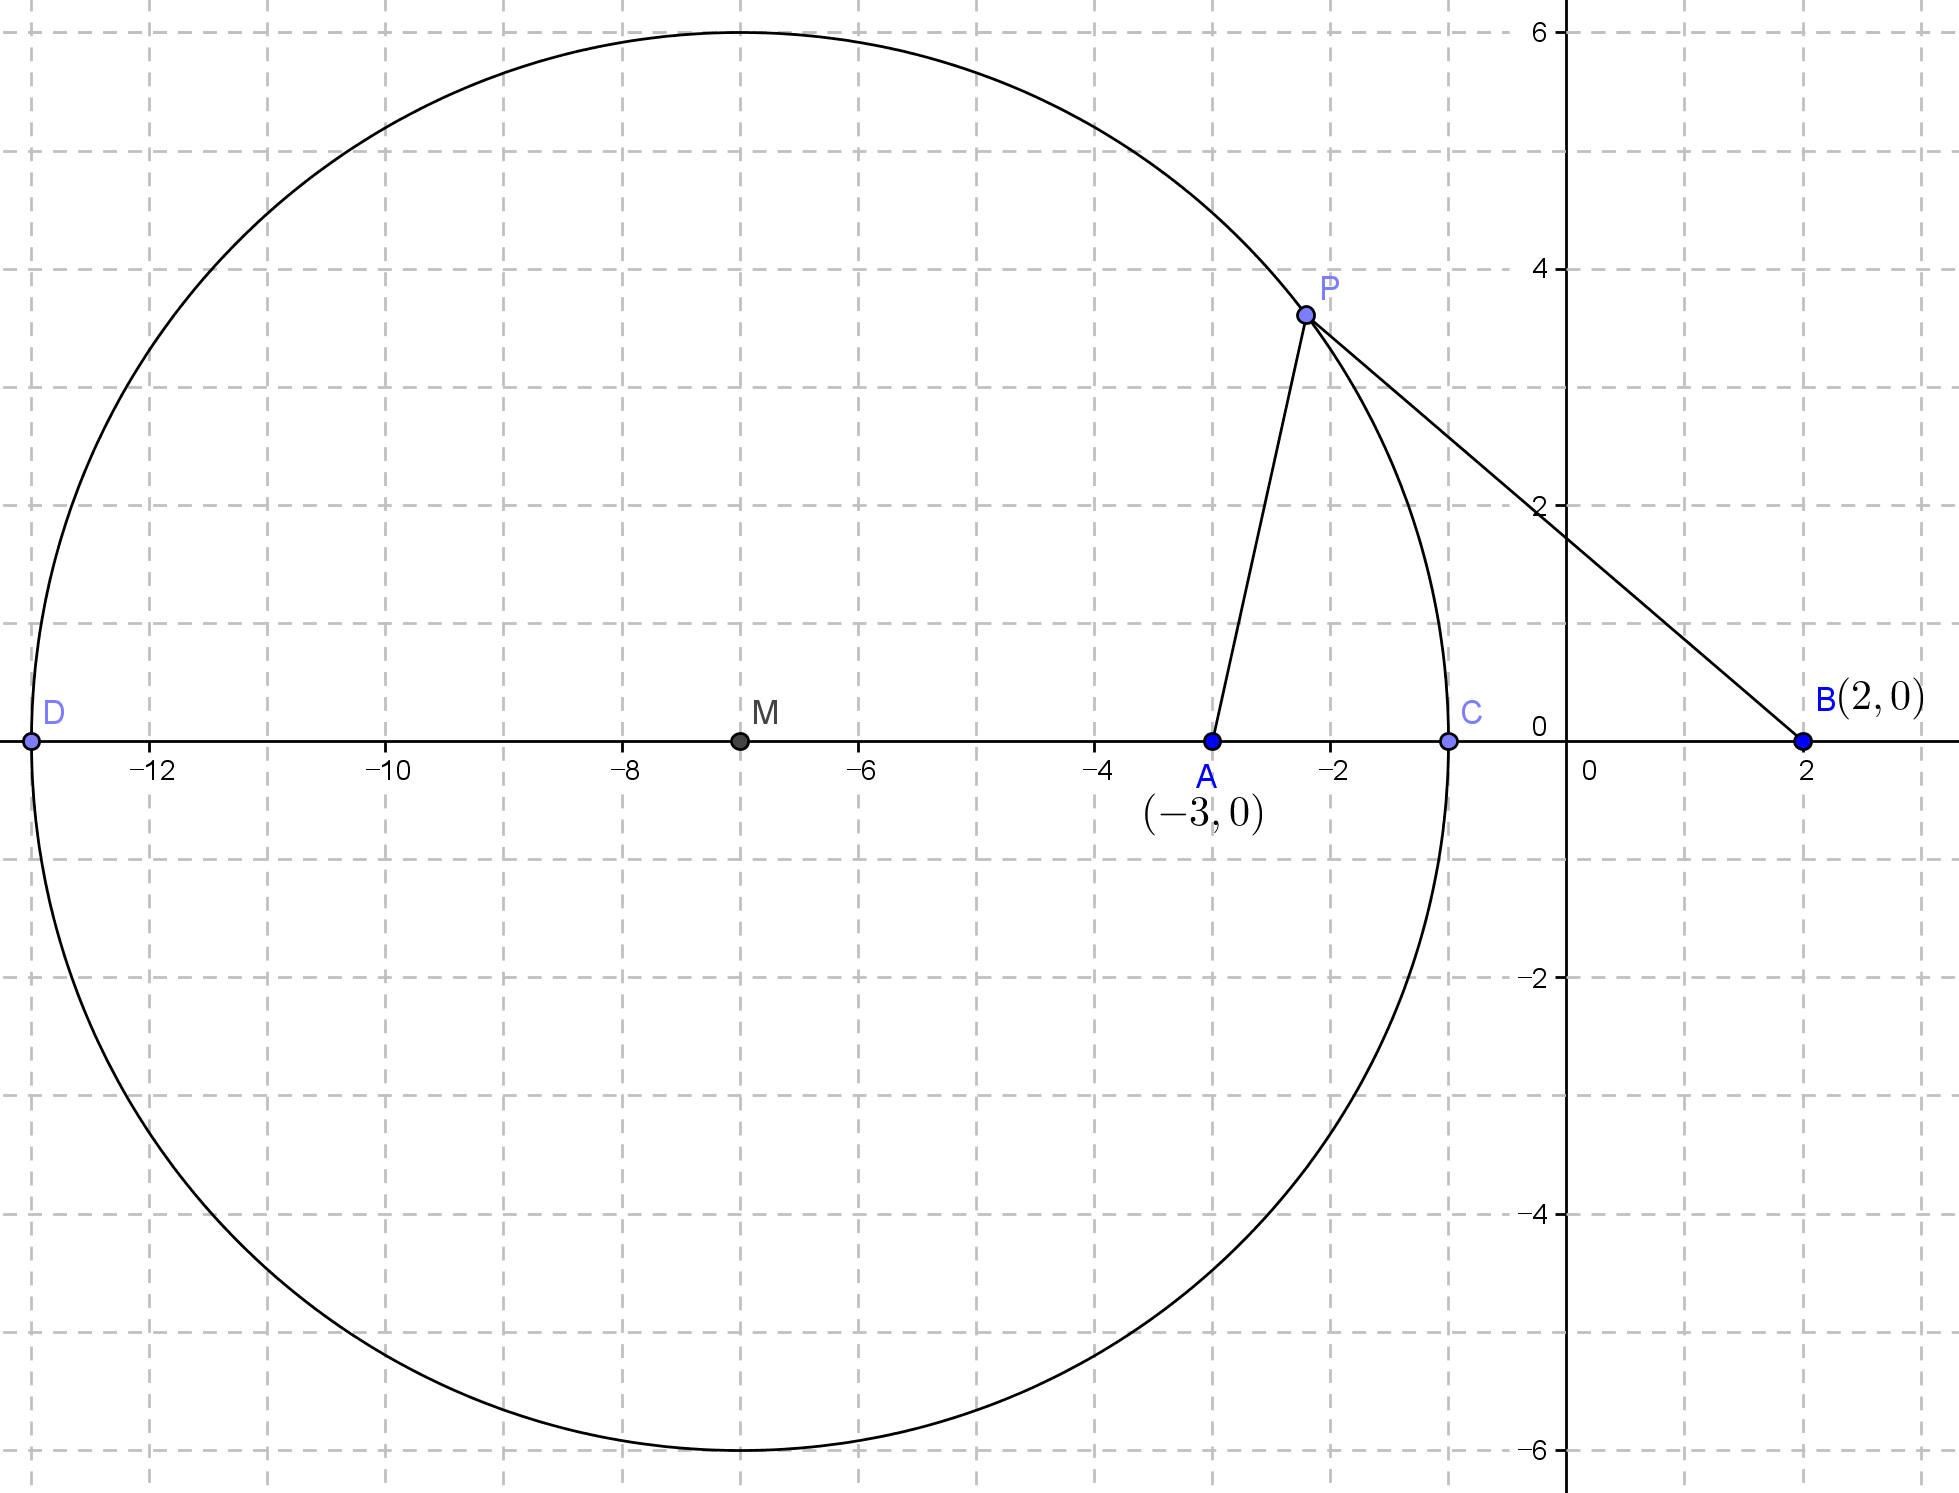
\includegraphics[width=0.7\textwidth]{appolonius}
\caption{\(\overline{AP}:\overline{BP}=2:3\)인 점 \(P\)의 자취}
\label{appolonius}
\end{figure}

%
\prob{}
두 점 \(A(-4,0)\), \(B(6,0)\)으로부터의 거리의 비가 \(2:3\)인 점 \(P\)가 나타내는 도형을 구하여라.

\ans{\((x+12)^2+y^2=144\)}

\section{원의 방정식(2)}

%
\summ{원과 직선 사이의 위치관계}
\begin{enumerate}
\item
직선과 원의 교점은 최대 두 개까지 존재할 수 있다.
교점이 2개면 이 직선을 할선이라고 부른다,
교점이 1개면 이 직선을 접선이라고 부르며, 이때의 교점을 접점이라고 부른다.
\item
원 \(x^2+y^2=r^2\)과 직선 \(ax+by+c=0\)의 교점의 개수는 다음 두 방법을 사용해 판별할 수 있다(그림 \ref{line-circle}).
\begin{enumerate}
\item
판별식을 이용하는 방법 :
두 도형 사이의 교점의 갯수는 두 식으로 만들어지는 연립방정식의 해의 갯수와 같으므로, 두 식을 연립하여 푼다.
연립할 때에 나타나는 이차방정식에서
(1) \(D>0\)이면 교점의 갯수가 두 개이고,
(2) \(D=0\)이면 교점의 갯수가 한 개이며,
(3) \(D<0\)이면 교점이 없다.
\item
점과 직선 사이의 거리를 이용하는 방법 :
원의 중심과 직선 사이의 거리를 \(d\)라고 하자.
(1) \(d<r\)이면  교점의 갯수가  두 개이고,
(2) \(d=r\)이면 교점의 갯수가 한 개이며,
(3) \(d<r\)이면 교점이 없다.
\end{enumerate}
\end{enumerate}

\begin{figure}[h]
\center
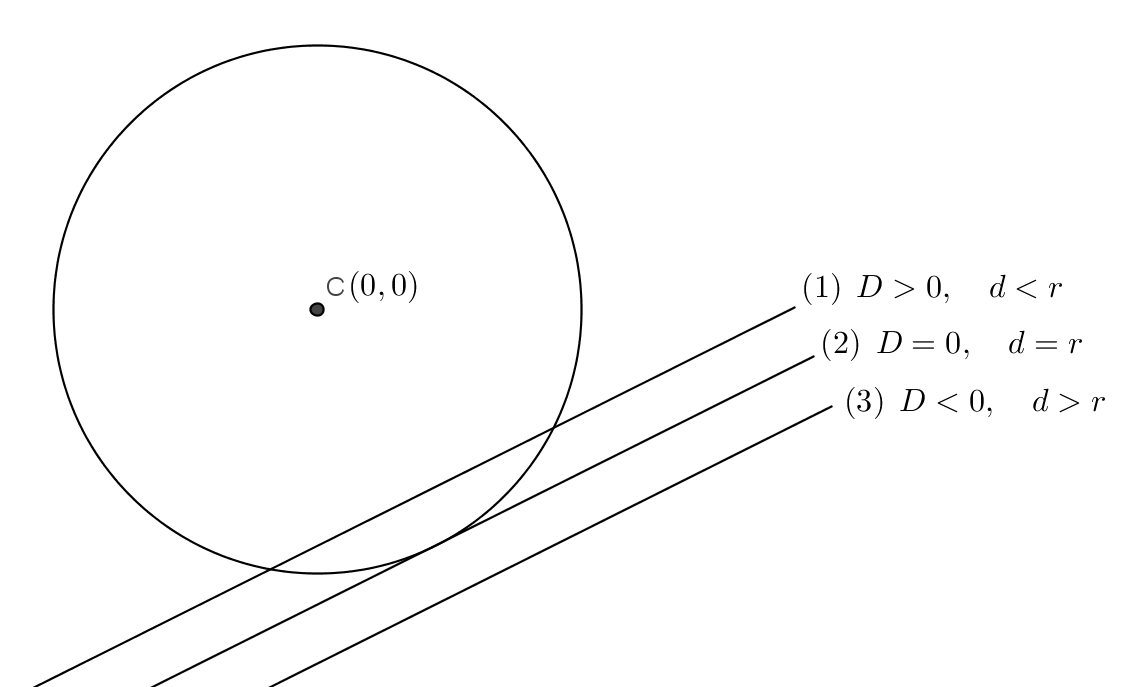
\includegraphics[width=\textwidth]{line-circle}
\caption{원과 직선 사이의 위치 관계}
\label{line-circle}
\end{figure}

%
\summ{}
\begin{enumerate}
\item
원 \(x^2+y^2=r^2\)에 접하고 기울기가 \(m\)인 접선의 방정식은 \(y=mx\pm r\sqrt{m^2+1}\)이다.
\item
원 \(x^2+y^2=r^2\) 위의 점 \((x_1,y_1)\)에서 그은 접선의 방정식은 \(x_1x+y_1y=r^2\)이다.
\end{enumerate}

%
\exam{}
다음 원과 직선의 교점의 개수를 구하여라.\\
(1) \(x^2+y^2=2\), \(y=x+1\)\\
(2) \(x^2+y^2=2\), \(y=x+2\)\\
(3) \(x^2+y^2=2\), \(y=x+3\)\\

\sol
\textbf{(판별식을 이용하는 방법)}
(1)
주어진 두 식을 연립하기 위해서 \(y=x+1\)을 \(x^2+y^2=2\)에 대입하면
\begin{gather*}
x^2+(x+1)^2=2\\
2x^2+2x-1=0
\end{gather*}
이 된다.
이때 \(D=2^2-4\times2\times(-1)>0\)이므로 교점은 두 개이다.

(2)
마찬가지의 방법을 쓰면
\begin{gather*}
x^2+(x+2)^2=2\\
2x^2+4x+2=0
\end{gather*}
이 된다.
이때 \(D=4^2-4\times2\times2=0\)이므로 교점은 한 개이다.

(3)
\begin{gather*}
x^2+(x+3)^2=2\\
2x^2+6x+7=0
\end{gather*}
이 된다.
이때 \(D=6^2-4\times2\times7<0\)이므로 교점은 없다.

\textbf{(점과 직선사이의 거리를 사용하는 방법)}

(1)
직선의 방정식을 변형하면 \(x-y+1=0\)이다.
원의 중심인 원점\((0,0)\)에서 이 직선까지의 거리는
\[d=\frac{|0-0+1|}{\sqrt{1^2+(-1)^2}}=\frac1{\sqrt2}\]
이므로 반지름 \(r=\sqrt2\)과 비교했을 때 \(d<r\)이다.
따라서 직선이 원에 충분히 가까이 있게 되어 교점이 두 개 존재한다.

(2)
마찬가지의 방법을 쓰면
\[d=\frac{|0-0+2|}{\sqrt{1^2+(-1)^2}}=\sqrt2\]
이므로 \(d=r\)이다.
따라서 교점이 한 개 존재하며 직선은 원에 접하게 된다.

(3)
\[d=\frac{|0-0+3|}{\sqrt{1^2+(-1)^2}}=\frac3{\sqrt2}\]
이므로 \(d>r\)이다.
따라서 직선이 원으로부터 너무 멀리 떨어져 있게 되어 교점이 존재하지 않는다(그림 \ref{x^2+y^2=2}).

\begin{figure}[h]
\center
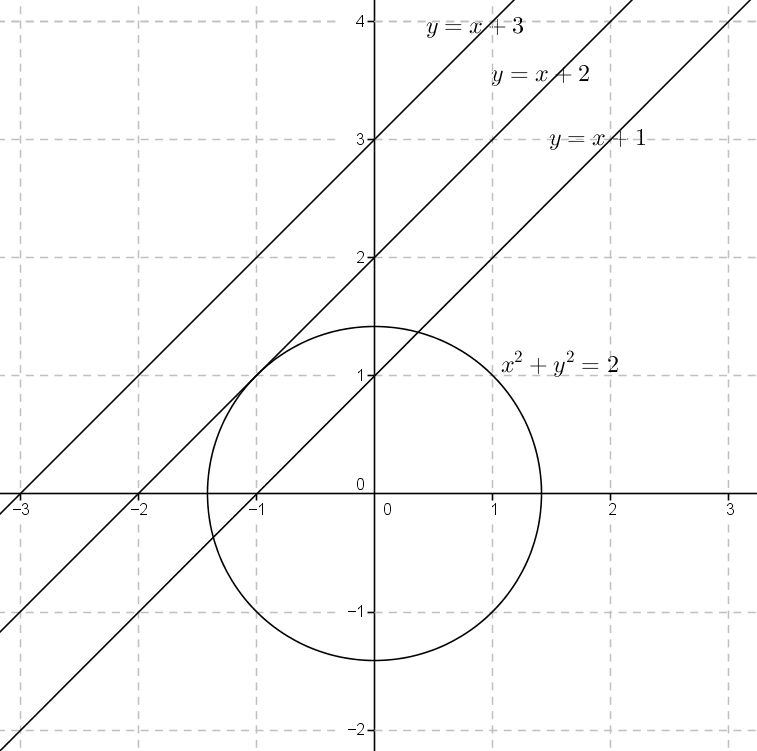
\includegraphics[width=0.4\textwidth]{x^2+y^2=2}
\caption{원 \(x^2+y^2=2\)와 세 직선 사이의 관계}
\label{x^2+y^2=2}
\end{figure}

%
\prob{}
다음 원과 직선의 교점의 개수를 구하여라.\\
(1) \(x^2+y^2=9\), \(y=-3x+5\)\\
(2) \(x^2+y^2=4\), \(x+2y-8=0\)

\ans{(1) 2개 (2) 0개}

%
\exam{}
다음 접선의 방정식을 구하여라.\\
(1) 원 \(x^2+y^2=4\)에 접하고 기울기가 \(-3\)인 접선\\
(2) 원 \(x^2+y^2=25\) 위의 점 \((3,-4)\)에서의 접선

\sol
(1)
공식
\[y=mx\pm r\sqrt{m^2+1}\]
에 \(m=-3\), \(r=2\)를 대입하면
\(y=-3x\pm2\sqrt{(-3)^2+1}\)이다.
이것을 정리하면
\(y=-3x\pm2\sqrt{10}\)이다.

\textbf{*(다른 방식의 풀이)}\\
위에 적힌 공식을 외우기가 너무 번거롭다고 하면, 다른 방법으로도 간편히 풀 수 있다.
(하지만 공식을 외우면 바로 풀 수 있다는 장점이 있다.)

기울기가 \(-3\)이므로 구하려는 접선의 방정식을 \(y=-3x+k\)라고 둘 수 있다.
이 접선의 방정식과 주어진 원의 방정식을 연립하기 위해 원의 방정식에 \(y=-3x+k\)를 대입하면
\begin{gather*}
x^2+(-3x+k)^2=4\\
10x^2-6kx+k^2-4=0
\end{gather*}
이다.
\(D=0\)이므로
\begin{gather*}
(-6k)^2-4\times10\times(k^2-4)=0\\
36k^2-40(k^2-4)\\
-4k^2+160=0\\
k^2=40\\
k=\pm2\sqrt{10}
\end{gather*}
이 된다.
따라서 구하려는 접선의 방정식은 \(y=-3x\pm2\sqrt{10}\)이고 이는 아까 구한 결과와 정확히 일치한다(그림 \ref{x^2+y^2=4}).

\begin{figure}[h]
\center
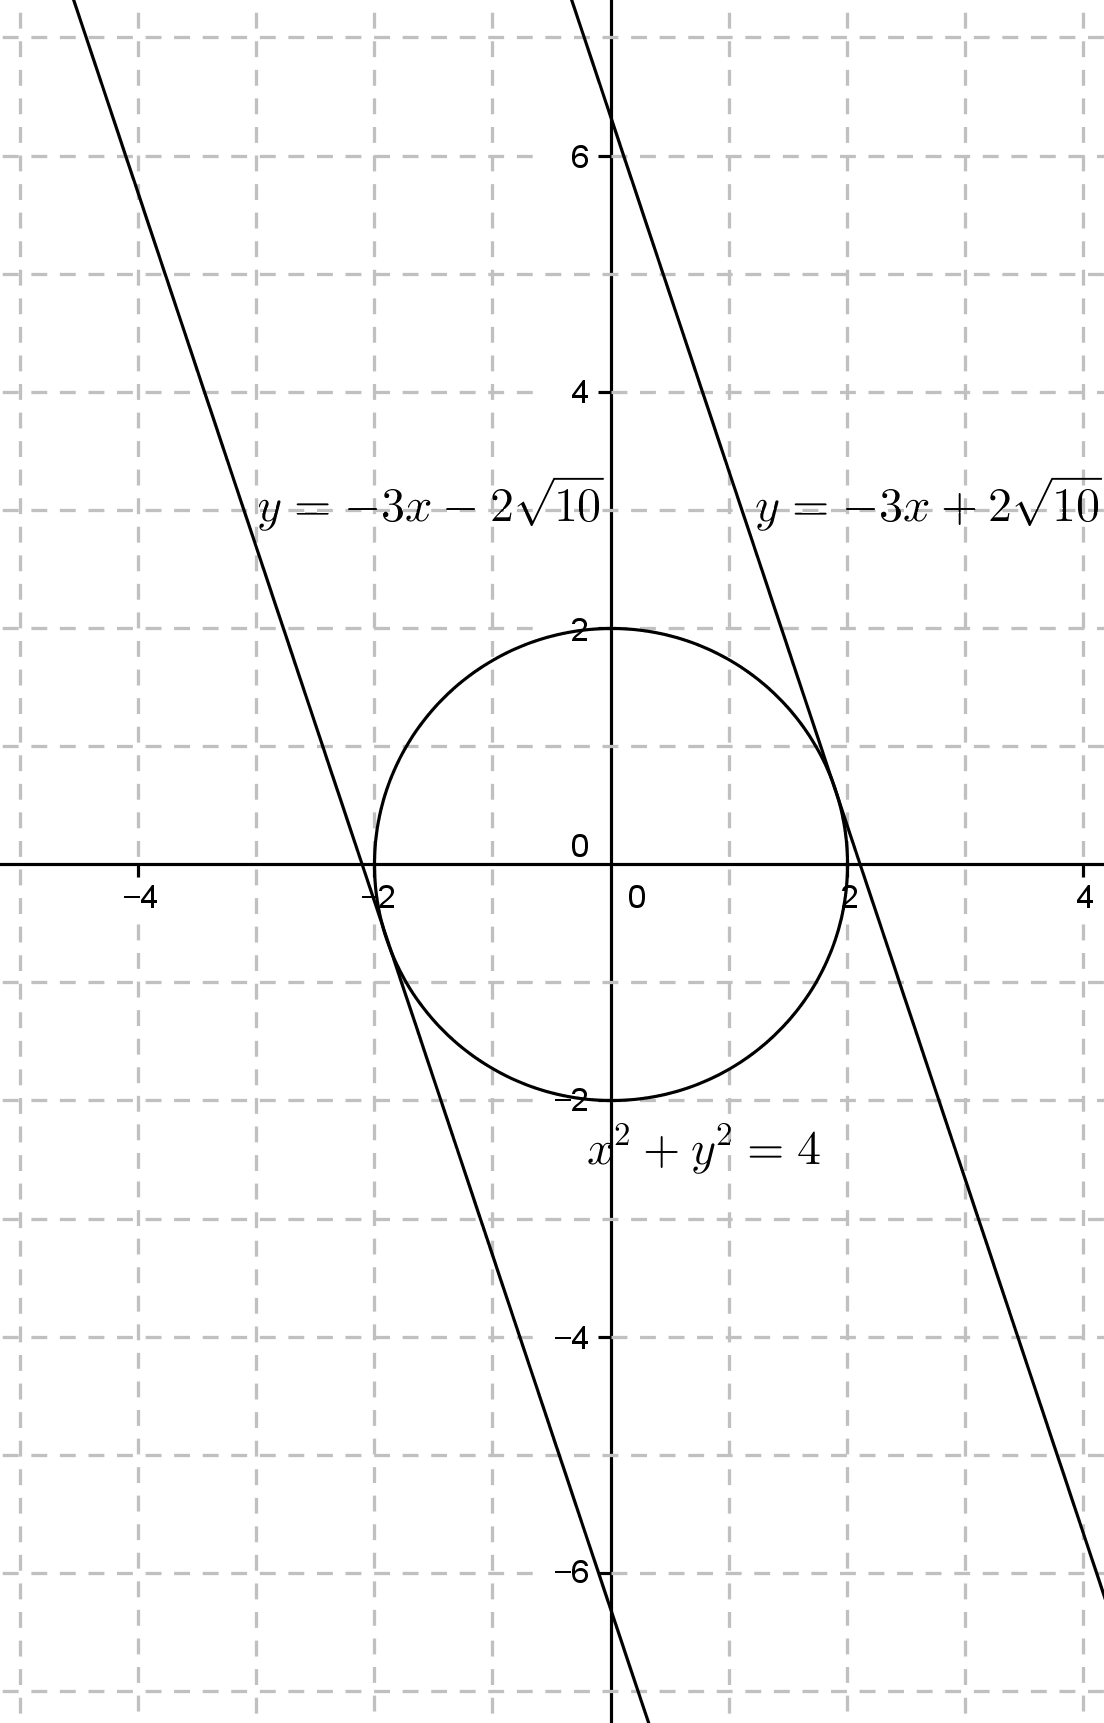
\includegraphics[width=0.4\textwidth]{x^2+y^2=4}
\caption{원 \(x^2+y^2=4\)에 접하고 기울기가 \(-3\)인 접선}
\label{x^2+y^2=4}
\end{figure}

(2)
공식
\[x_1x+y_1y=r^2\]
에 \((x_1,y_1)=(3,-4)\), \(r=5\)를 대입하면
\(3x-4y=25\)이다.

\begin{figure}[h]
\center
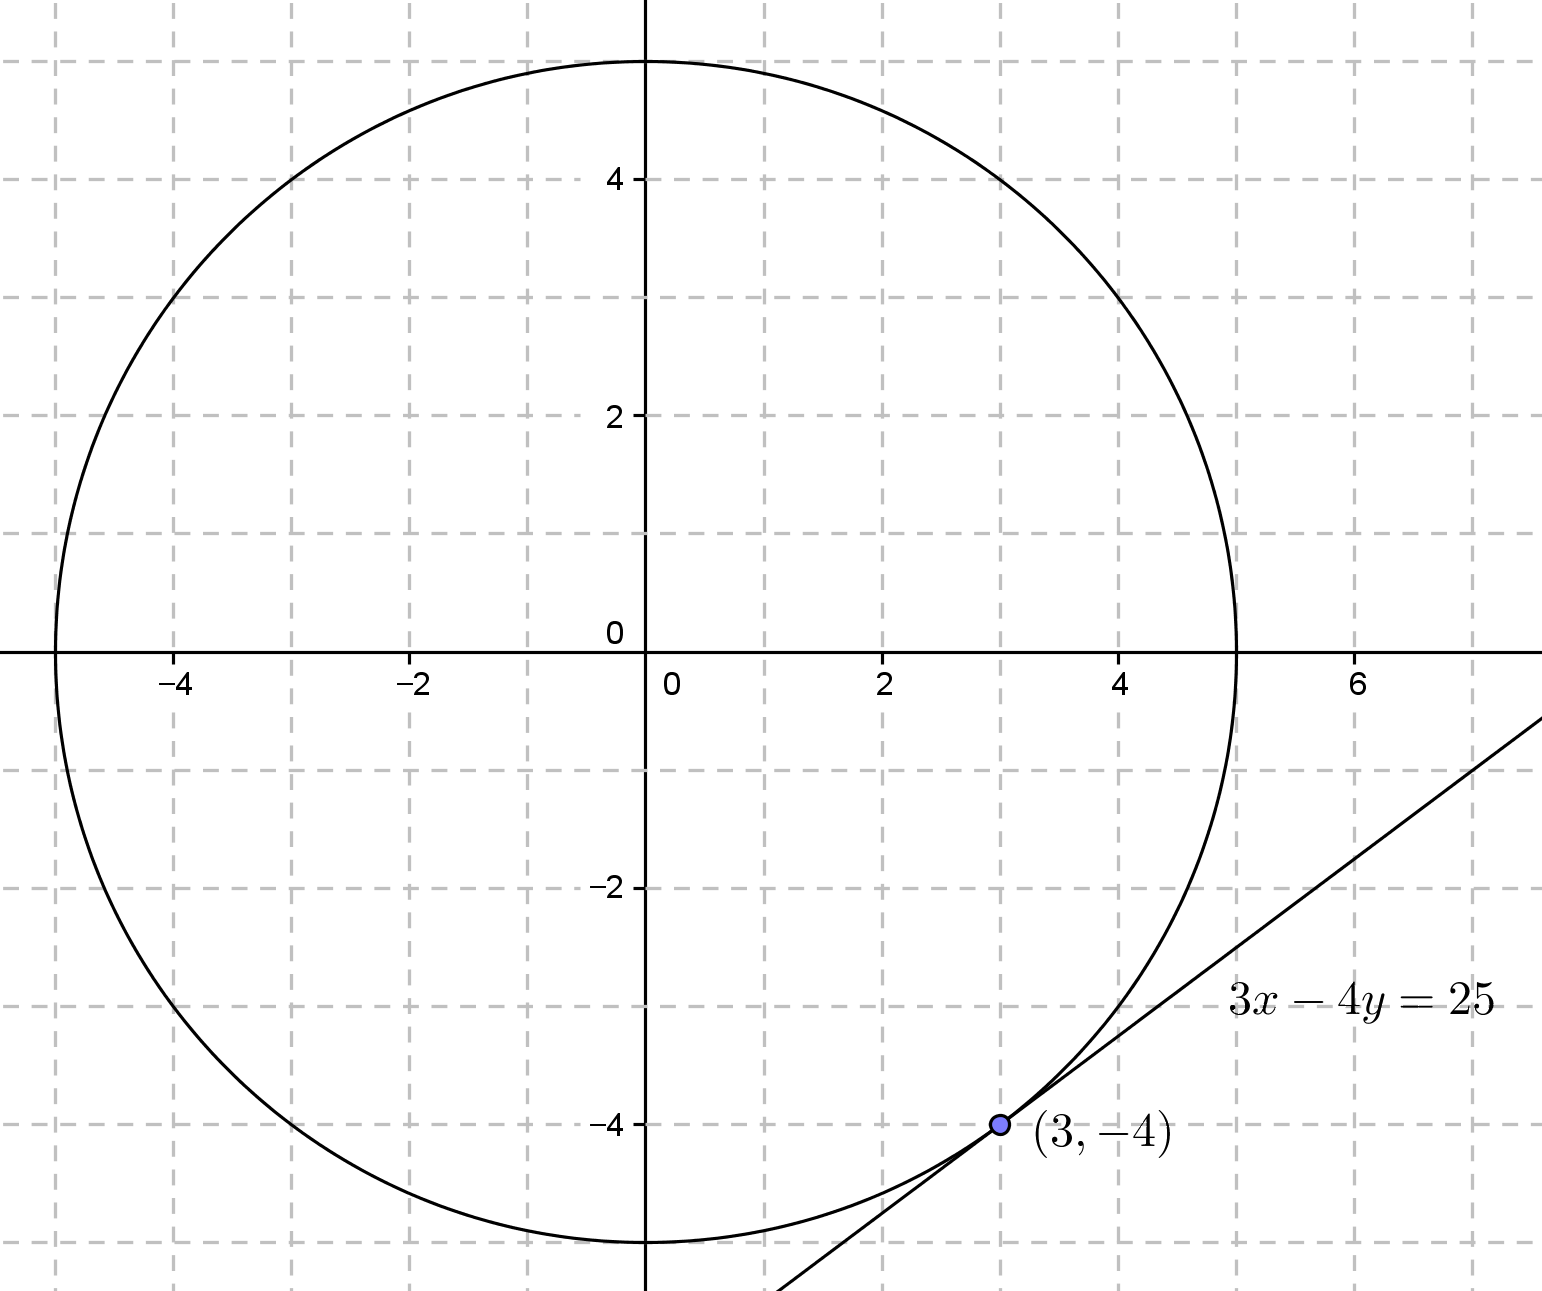
\includegraphics[width=0.4\textwidth]{x^2+y^2=25}
\caption{원 \(x^2+y^2=25\) 위의 점 \((3,-4)\)에서의 접선}
\label{x^2+y^2=25}
\end{figure}

%
\prob{}
다음 접선의 방정식을 구하여라.\\
(1) 원 \(x^2+y^2=5\)에 접하고 기울기가 \(-3\)인 접선\\
(2) 원 \(x^2+y^2=25\)위의 점 \((-3,4)\)에서 그은 접선

\ans{
(1) \(y=-3x\pm5\sqrt2\)\\
(2) \(-3x+4y=25\)
}

%
\exam{}
점 \(A(1,3)\)에서 원 \(x^2+y^2=5\)에 그은 접선의 방정식을 구하여라.

\sol
\textbf{(공식 \(x_1x+y_1y=r^2\)을 이용하는 방법)}\\
접점을 \(P(x_1,y_1)\)이라고 하면 \(P\)는 원 \(x^2+y^2=5\) 위의 점이므로
\begin{equation}
{x_1}^2+{y_1}^2=5
\end{equation}
가 성립한다.
또한 접선은 \(x_1x+y_1y=5\)인데 이 접선이 \(A(1,3)\)을 지나므로
\begin{equation}
x_1+3y_1=5
\end{equation}
가 성립한다.
(1)과 (2)를 연립하기 위해 (2)를
\[x_1=5-3y_1\]
으로 변형한 후 (1)에 대입하자.
그러면
\begin{gather*}
(5-3y_1)^2+{y_1}^2=5\\
10{y_1}^2-30y_1+20=0\\
{y_1}^2-3y_1+2=0\\
(y_1-1)(y_1-2)=0
\end{gather*}
이므로 \(y_1=1\) 또는 \(y_1=2\)이다.
\(y_1=1\)이면 식 (2)로부터 \(x_1=2\)이고, \(y_1=2\)이면 \(x_1=-1\)이다.
즉
\[(x_1,y_1)=(2,1),(-1,2)\]
이다.
이것을
\[x_1x+y_1y=5\]
에 각각 대입하면 두 접선이
\begin{gather*}
2x+y=5\\
-x+2y=5
\end{gather*}
임을 알 수 있다.

\textbf{(공식 \(y-y_1=m(x-x_1)\)을 이용하는 방법)}\\
접선의 기울기를 \(m\)이라고 하면 구하려는 접선의 방정식은
\begin{equation}
y-3=m(x-1)
\end{equation}
이다.
즉
\[mx-y+3-m=0\]
이다.
이 직선과 원의 중심 \((0,0)\)까지의 거리가 반지름인 \(\sqrt5\)와 같으므로
\[\sqrt5=\frac{|3-m|}{\sqrt{m^2+1}}\]
이 성립한다.
양변에 \(\sqrt{m^2+1}\)를 곱하면
\[\sqrt5\sqrt{m^2+1}=|3-m|\]
이고 이 식의 양변을 제곱하면
\[5m^2+5=m^2-6m+9\]
가 된다.
이것을 다시 정리하면
\begin{align*}
4m^2+6m-4&=0\\
2m^2+3m-2&=0\\
(m+2)(2m-1)&=0
\end{align*}
이 되어 \(m=-2\)이거나 \(m=\frac12\)이다.

이 값들을 (3)에 대입하면
\begin{gather*}
y-3=-2(x-1)\\
y-3=\frac12(x-1)
\end{gather*}
혹은
\begin{gather*}
y=-2x+5\\
y=\frac12x+\frac52
\end{gather*}
를 얻는다.
이는 첫번째 방법으로 얻은 결과와 정확히 일치한다.

\begin{figure}[h]
\center
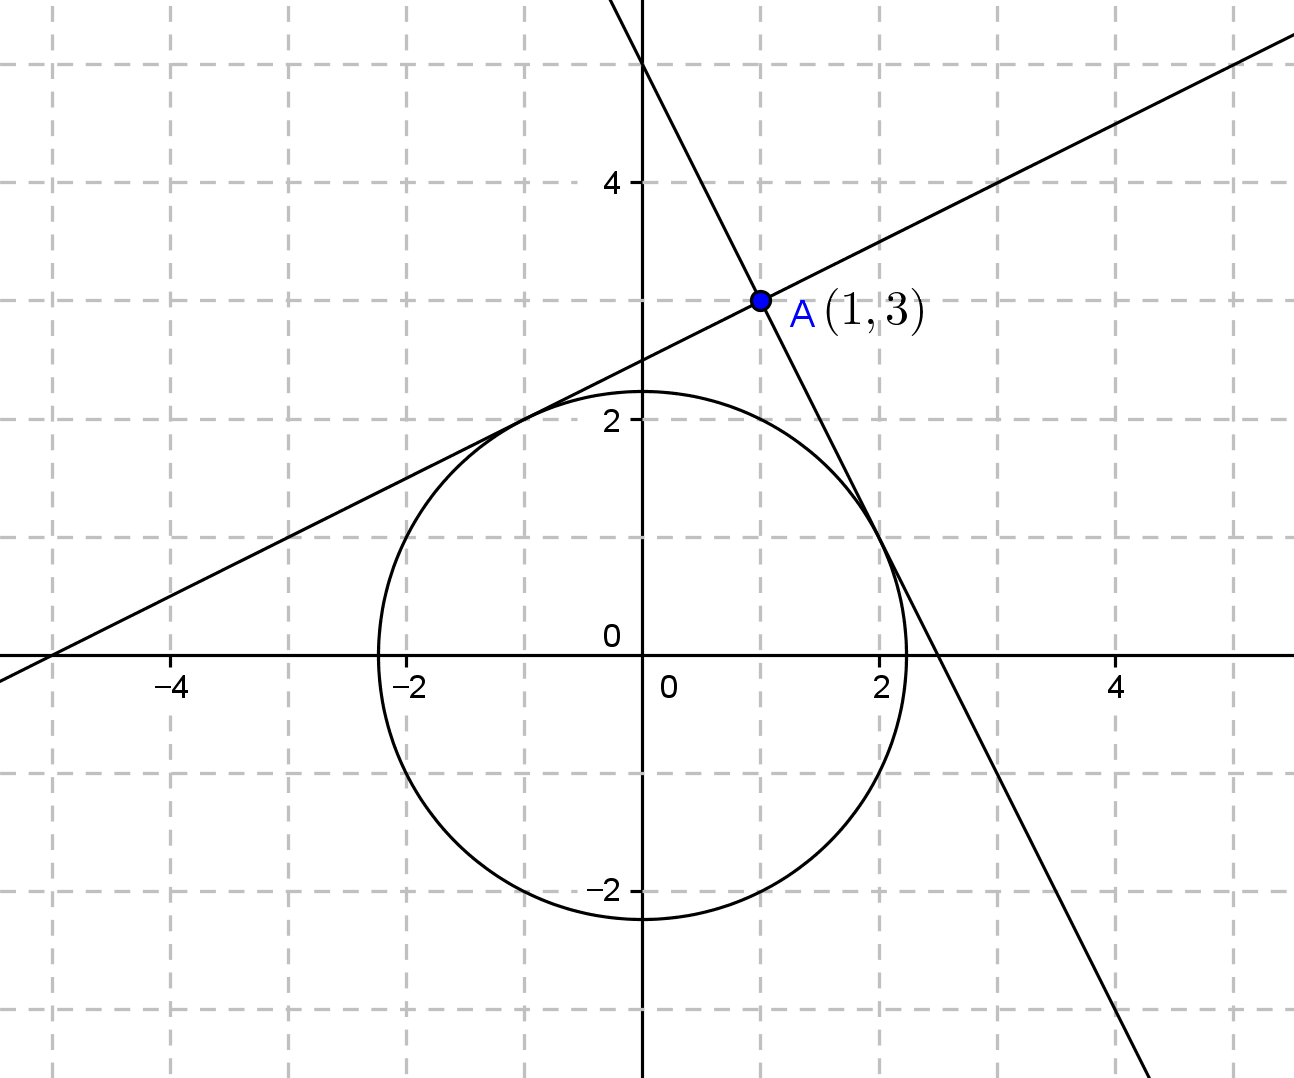
\includegraphics[width=0.4\textwidth]{x^2+y^2=5}
\caption{점 \((1,3)\)에서 원 \(x^2+y^2=5\)에 그은 접선}
\label{x^2+y^2=5}
\end{figure}

\prob{}
다음 점에서 주어진 원에 그은 접선의 방정식을 구하여라.\\
(1) 점 \((2,0)\), \(x^2+y^2=2\)\\
(2) 점 \((7,1)\), \(x^2+y^2=25\)

\ans{
(1) \(x+y=2\) 또는 \(x-y=2\)\\
(2) \(3x+4y=25\) 또는 \(4x-3y=25\)
}


%%
\section{도형의 이동}

%
\summ{}
\begin{enumerate}
\item
좌표평면 위의 점 \(P(x,y)\)를
\begin{enumerate}
\item
\(x\)축으로 \(a\)만큼, \(y\)축으로 \(b\)만큼 평행이동 시키면 \((x+a,y+b)\)이 된다.
\item
\(x\)축에 대해 대칭이동시키면 \((x,-y)\)가 된다.
\item
\(y\)축에 대해 대칭이동시키면 \((-x,y)\)가 된다.
\item
원점에 대해 대칭이동시키면 \((-x,-y)\)가 된다.
\item
\(y=x\)에 대해 대칭이동시키면 \((y,x)\)가 된다.
\end{enumerate}
\item
좌표평면 위의 도형 \(f(x,y)=0\)을
\begin{enumerate}
\item
\(x\)축으로 \(a\)만큼, \(y\)축으로 \(b\)만큼 평행이동 시키면 \(f(x-a,y-b)=0\)이 된다.
(\(x\) 대신에 \(x-a\)를 대입하고 \(y\) 대신에 \(y-b\)를 대입한다.)
\item
\(x\)축에 대해 대칭이동시키면 \(f(x,-y)=0\)가 된다.
(\(y\) 대신에 \(-y\)를 대입한다.)
\item
\(y\)축에 대해 대칭이동시키면 \(f(-x,y)=0\)가 된다.
(\(x\) 대신에 \(-x\)를 대입한다.)
\item
원점에 대해 대칭이동시키면 \(f(-x,-y)=0\)가 된다.
(\(x\) 대신에 \(-x\)를 대입하고 \(y\) 대신에 \(-y\)를 대입한다.)
\item
\(y=x\)에 대해 대칭이동시키면 \(f(y,x)=0\)가 된다.
(\(x\) 대신에 \(y\)를 대입하고 \(y\) 대신에 \(x\)를 대입한다.)
\end{enumerate}
\end{enumerate}

%
\exam{}
점 \((3,4)\)를 다음과 같이 이동시켰을 때의 좌표를 구하여라.\\
(1) \(x\)축 방향으로 \(2\)만큼, \(y\)축 방향으로 \(-3\) 대칭이동\\
(2) \(x\)축에 대해 대칭이동\\
(3) \(y\)축에 대해 대칭이동\\
(4) 원점에 대해 대칭이동\\
(5) \(y=x\)에 대해 대칭이동

\sol
각각 \\
(1) \((3+2,4-3)=(5,1)\)\\
(2) \((3,-4)\)\\
(3) \((-3,4)\)\\
(4) \((-3,-4)\)\\
(5) \((4,3)\)\\
으로 이동된다.

%
\prob{}
점 \((-2,5)\)를 다음과 같이 이동시켰을 때의 좌표를 구하여라.\\
(1) \(x\)축 방향으로 \(2\)만큼, \(y\)축 방향으로 \(-3\) 대칭이동\\
(2) \(x\)축에 대해 대칭이동\\
(3) \(y\)축에 대해 대칭이동\\
(4) 원점에 대해 대칭이동\\
(5) \(y=x\)에 대해 대칭이동

\ans{
(1) \((0,2)\) (2) \((-2,-5)\) (3) \((2,5)\) (4) \((2,-5)\) (5) \((5,-2)\)
}

%
\exam{}
직선 \(2x-y+1=0\)을 다음과 같이 이동시켰을 때의 식을 구하여라.\\
(1) \(x\)축 방향으로 \(2\)만큼, \(y\)축 방향으로 \(-3\) 대칭이동\\
(2) \(x\)축에 대해 대칭이동\\
(3) \(y\)축에 대해 대칭이동\\
(4) 원점에 대해 대칭이동\\
(5) \(y=x\)에 대해 대칭이동

\sol
(1) \(x\) 대신에 \(x-2\)를, \(y\) 대신에 \(y+3\)을 넣으면 되므로
\begin{gather*}
2(x-2)-(y+3)+1=0\\
2x-y-6=0
\end{gather*}
이다.

(2) \(y\) 대신에 \(-y\)를 넣으면 되므로
\begin{gather*}
2x-(-y)+1=0\\
2x+y+1=0
\end{gather*}
이다.

(3) \(x\) 대신에 \(-x\)를 넣으면 되므로
\begin{gather*}
2(-x)-y+1=0\\
-2x-y+1=0
\end{gather*}
이다.

(4) \(x\) 대신에 \(-x\)를, \(y\) 대신에 \(-y\)를 넣으면 되므로
\begin{gather*}
2(-x)-(-y)+1=0\\
-2x+y+1=0
\end{gather*}
이다.

(5) \(x\) 대신에 \(y\)를, \(y\) 대신에 \(x\)를 넣으면 되므로
\begin{gather*}
2(y)-(x)+1=0\\
-x+2y+1=0
\end{gather*}
이다(그림 \ref{2x-y+1=0}).

\begin{figure}[h]
\center
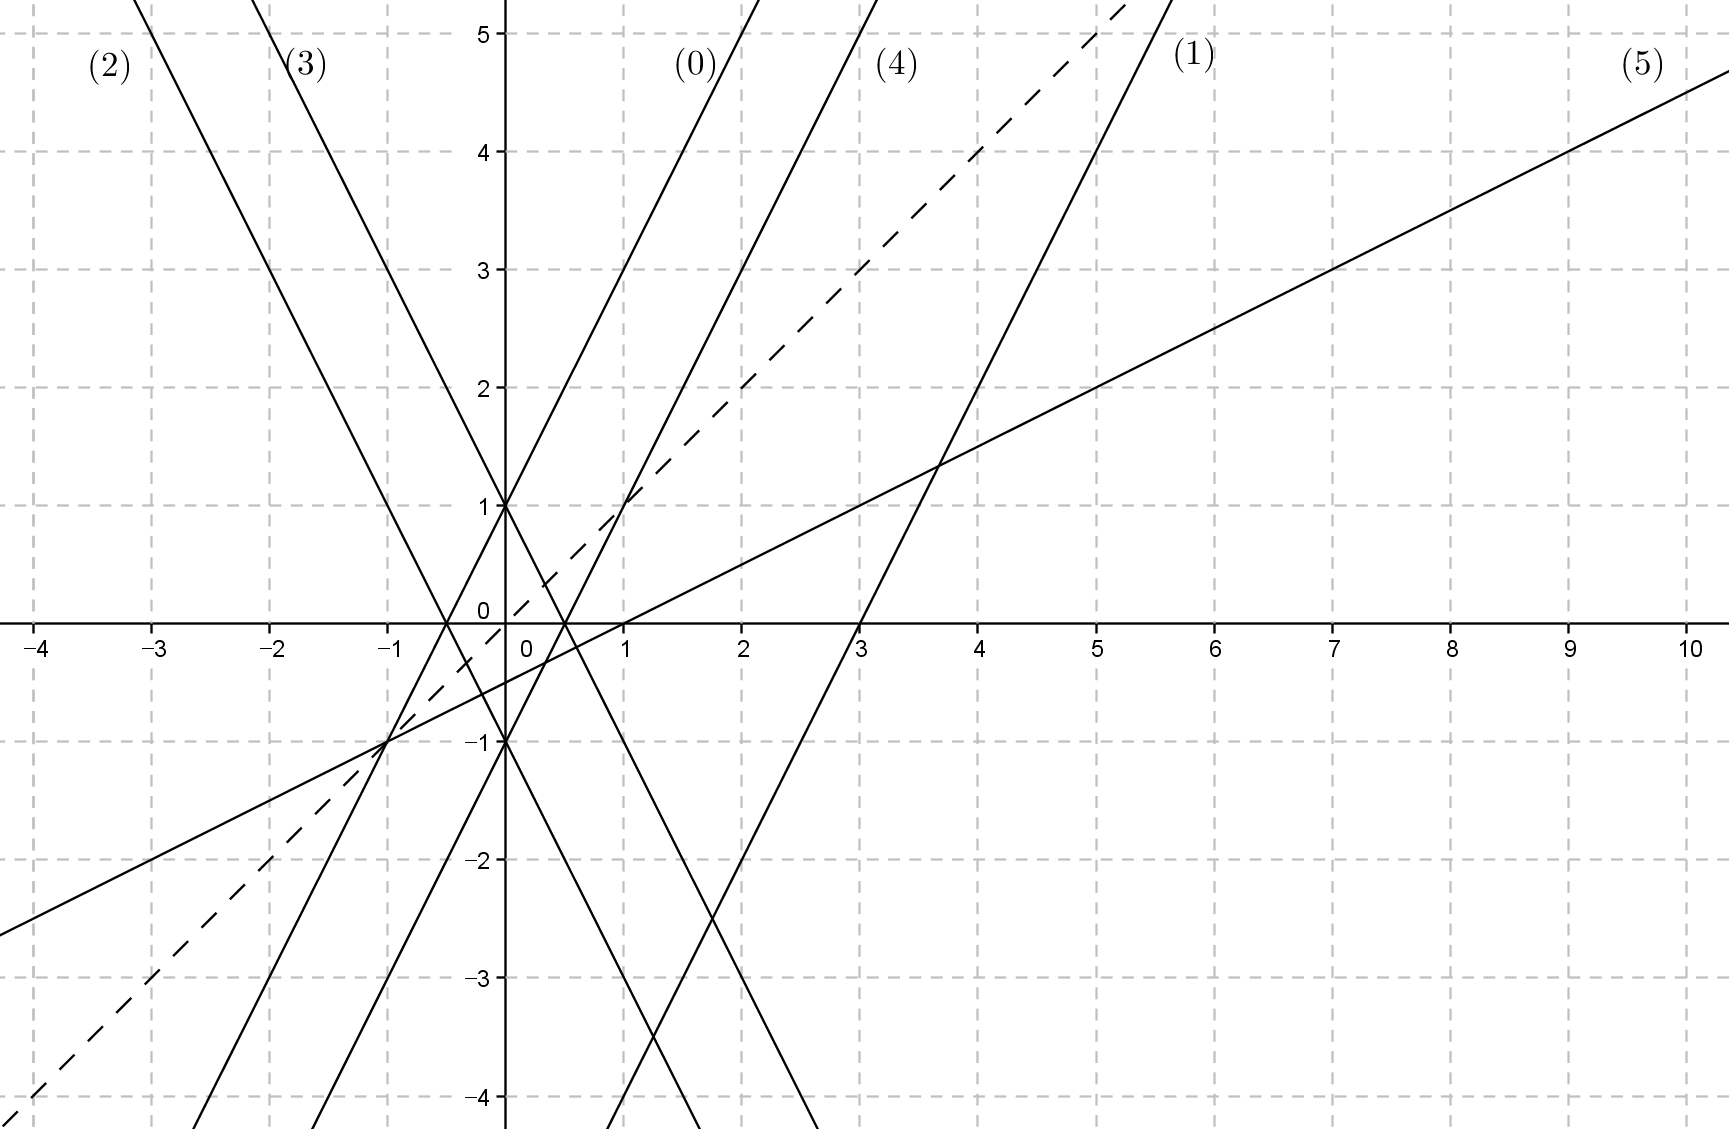
\includegraphics[width=0.9\textwidth]{2x-y+1=0}
\caption{\(2x-y+1=0\)를 이동시킨 그래프들, (0)은 원래의 직선.}
\label{2x-y+1=0}
\end{figure}


%
\exam{}
원 \((x-3)^2+(y-2)^2=1\)을 다음과 같이 이동시켰을 때의 식을 구하여라.\\
(1) \(x\)축 방향으로 \(2\)만큼, \(y\)축 방향으로 \(-3\) 대칭이동\\
(2) \(x\)축에 대해 대칭이동\\
(3) \(y\)축에 대해 대칭이동\\
(4) 원점에 대해 대칭이동\\
(5) \(y=x\)에 대해 대칭이동

\sol
아까와 같은 방법으로 구하면\\
(1) \((x-5)^2+(y+1)^2=1\)\\
(2) \((x-3)^2+(y+2)^2=1\)\\
(3) \((x+3)^2+(y-2)^2=1\)\\
(4) \((x+3)^2+(y+2)^2=1\)\\
(5) \((x-2)^2+(y-3)^2=1\)
이다(그림 \ref{axises}).

\begin{figure}[h]
\center
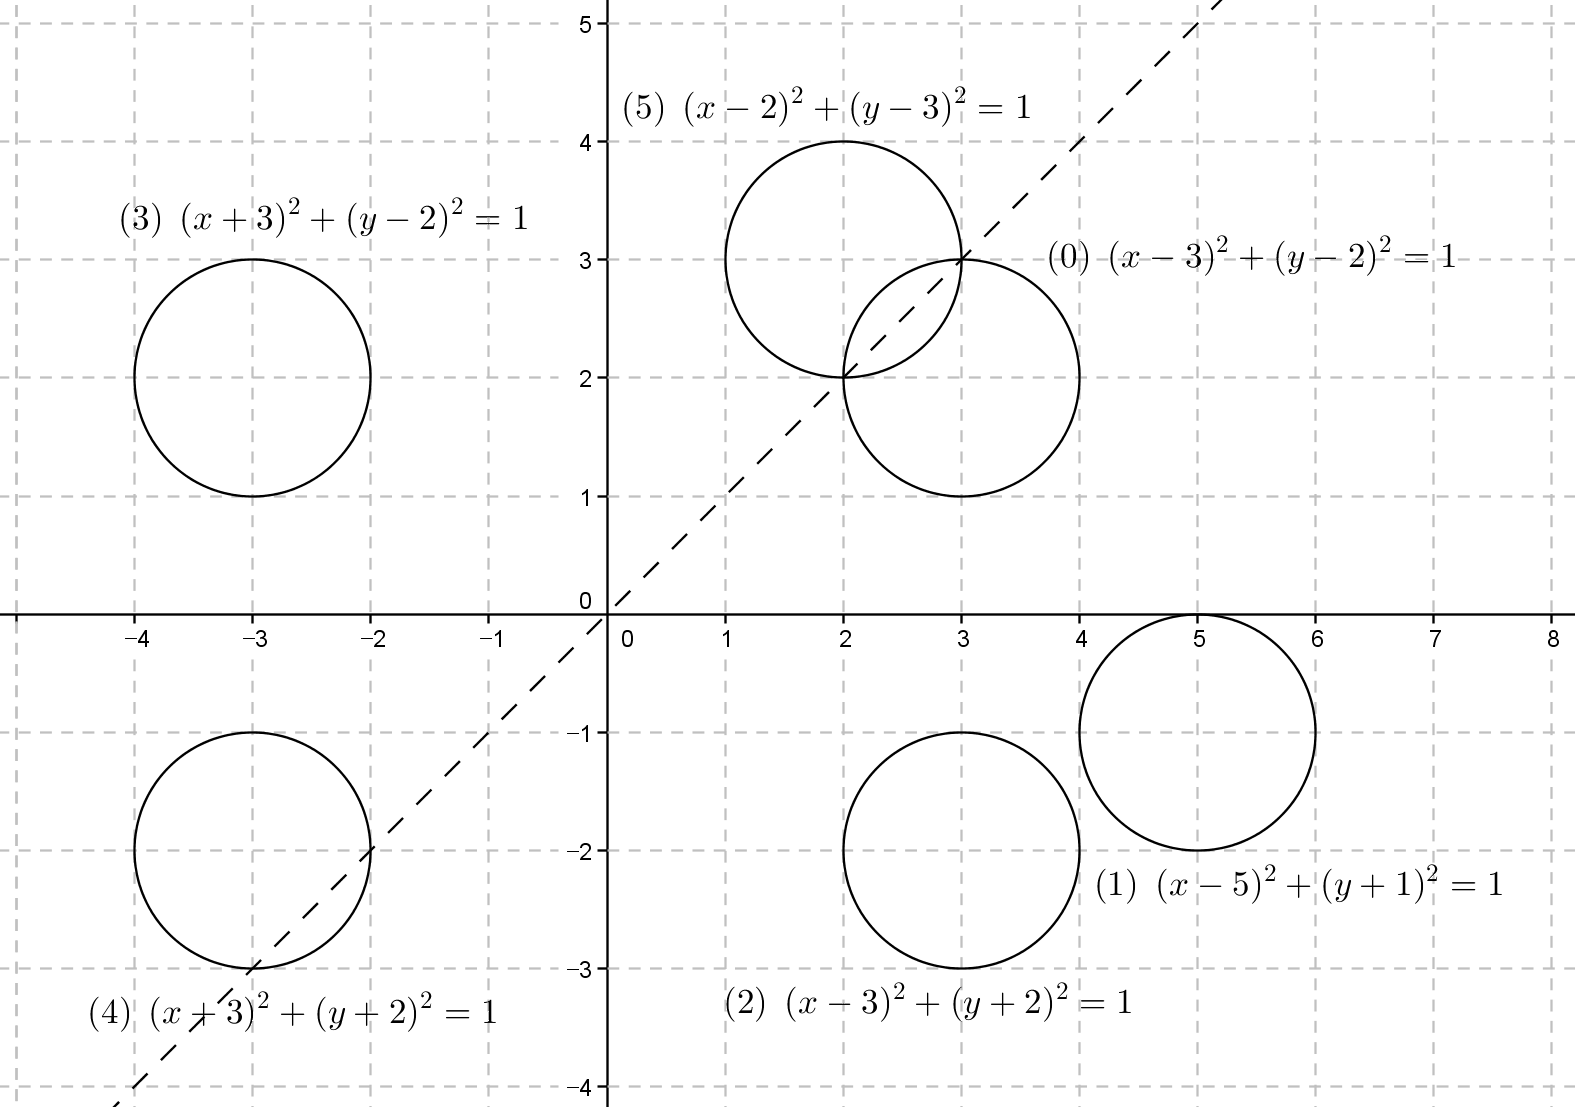
\includegraphics[width=0.9\textwidth]{axises}
\caption{\((x-3)^2+(y-2)^2=1\)를 이동시킨 그래프들, (0)은 원래의 원.}
\label{axises}
\end{figure}

\exam{}
좌표평면 위의 두 점 \(A(1,2)\), \(B(4,6)\)에 대하여 점 \(P\)가 \(y\)축 위를 움직일 때, \(\overline{AP}+\overline{BP}\)의 최솟값을 구하여라.

\sol
\(A\)를 \(y\)축에 대해 대칭이동한 점을 \(A'\)이라고 하면 \(A'=(-1,2)\)이다.
\(\overline{AP}=\overline{A'P}\)이므로 \(\overline{AP}+\overline{BP}\)의 최솟값을 구하는 대신, \(\overline{A'P}+\overline{BP}\)의 최솟값을 구해도 된다.
그런데 \(\overline{A'P}+\overline{BP}\)는 \(A'\)에서 \(x\)축 위의 점 \(P\)를 거쳐 \(B\)로 가는 거리이므로 \(A'\)에서 \(B\)로 이은 직선거리가 최솟값이 된다.
따라서 구하고자 하는 최솟값은 \(\overline{A'B}=\sqrt{5^2+4^2}=\sqrt{41}\)이다(그림 \ref{APBP}).

\begin{figure}[h]
\center
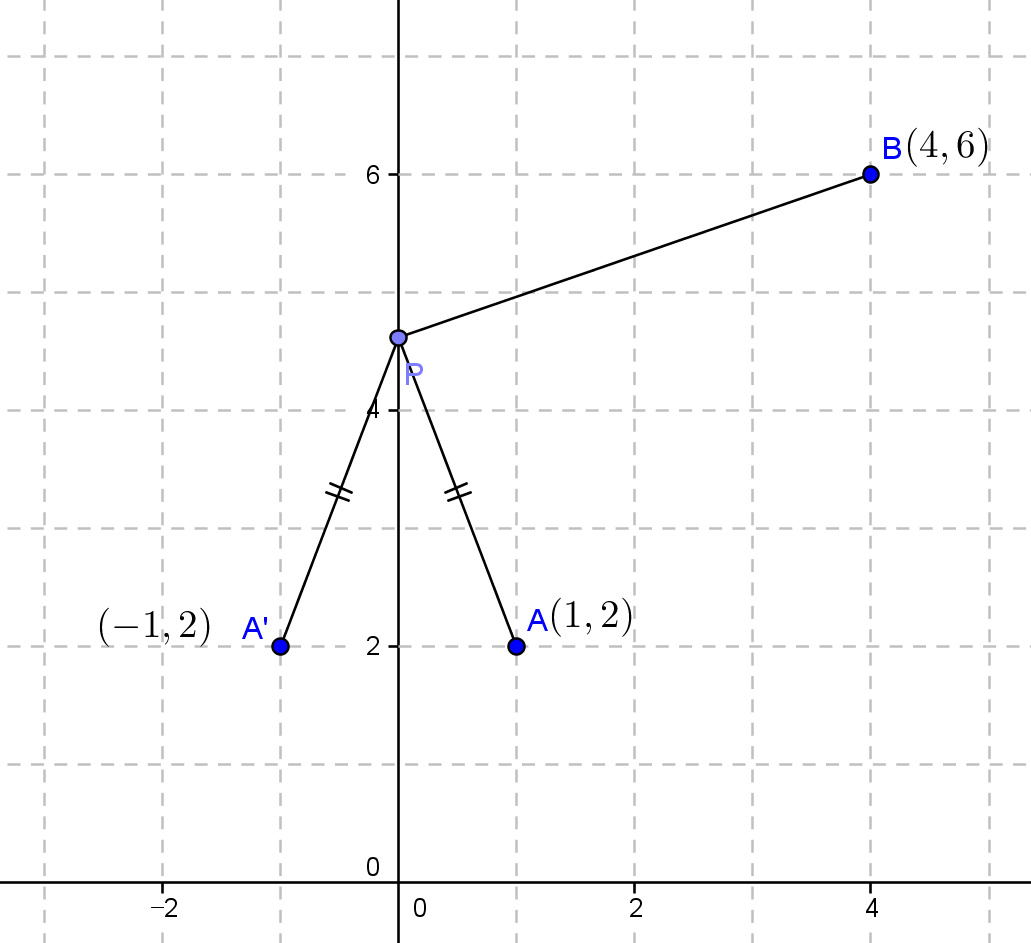
\includegraphics[width=0.4\textwidth]{APBP}
\caption{대칭이동을 이용한 최솟값 구하기}
\label{APBP}
\end{figure}

%
\prob{}
좌표평면 위의 두 점 \(A(4,1)\), \(B(7,4)\)에 대하여 점 \(P\)가 \(y=x\) 위를 움직일 때, \(\overline{AP}+\overline{BP}\)의 최솟값을 구하여라.

\ans{
최솟값=\(6\)
}




%%
\section{부등식의 영역}

%
\summ{}
\begin{enumerate}
\item
함수 \(f\)에 대해 부등식이 나타내는 영역은 다음과 같이 표시된다.
\par
\bigskip
\noindent
{\footnotesize
\begin{tabular}{p{0.24\textwidth}|p{0.24\textwidth}|p{0.24\textwidth}|p{0.24\textwidth}}
\hline
\(y>f(x)\)	&\(y\ge f(x)\)	&\(y< f(x)\)	&\(y\le f(x)\)\\
\hline
\raisebox{-.5\height}{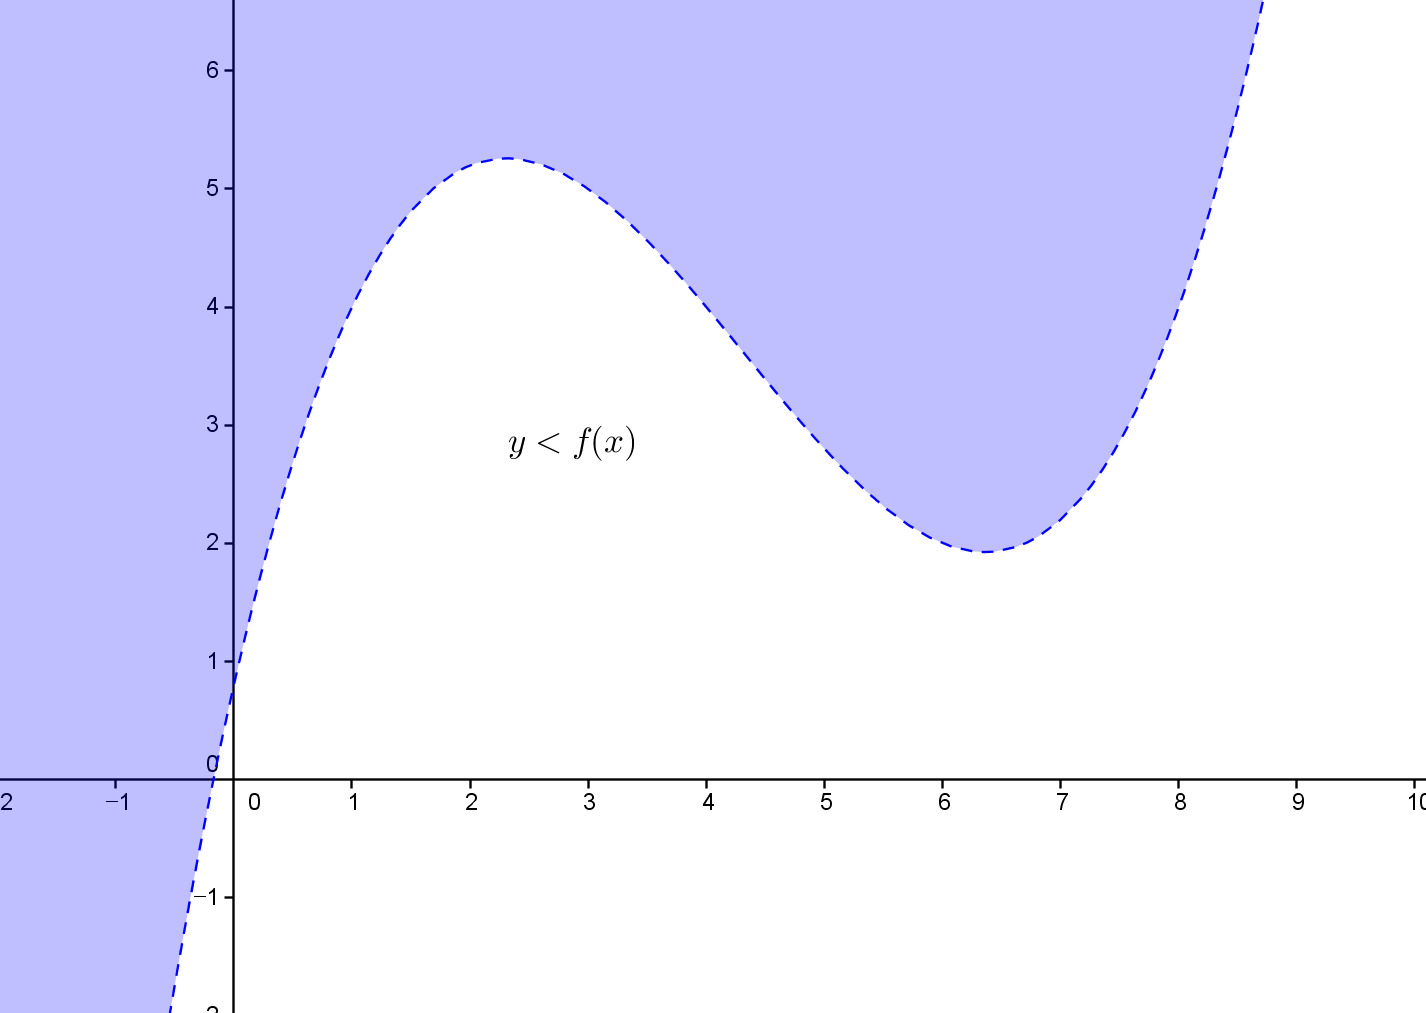
\includegraphics[width=0.24\textwidth]{ineq_1}}
&\raisebox{-.5\height}{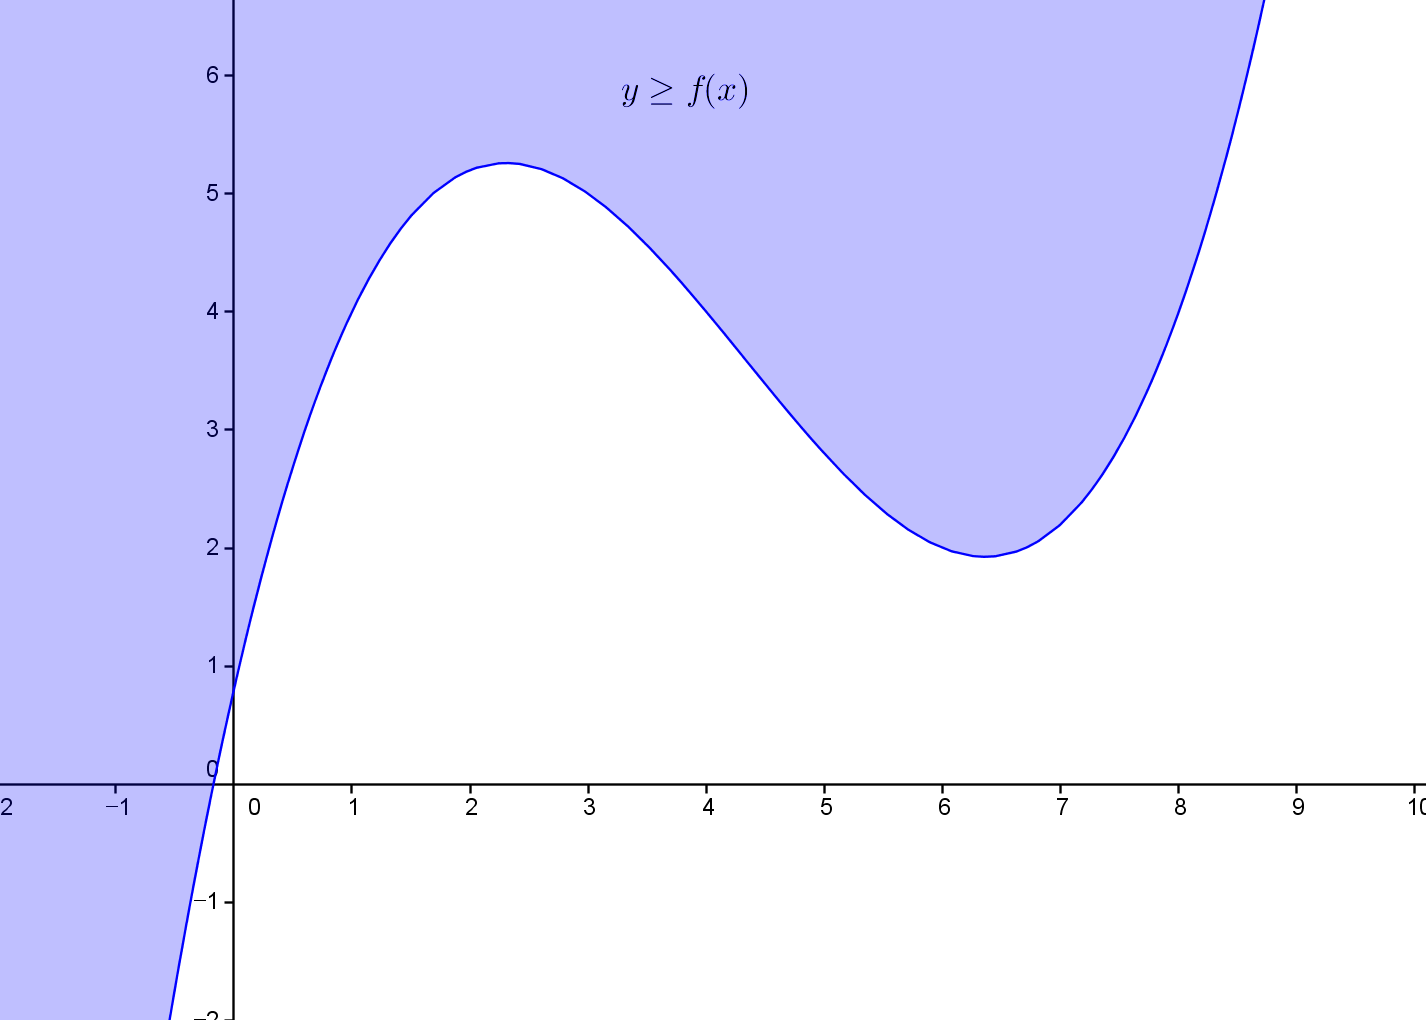
\includegraphics[width=0.24\textwidth]{ineq_2}}
&\raisebox{-.5\height}{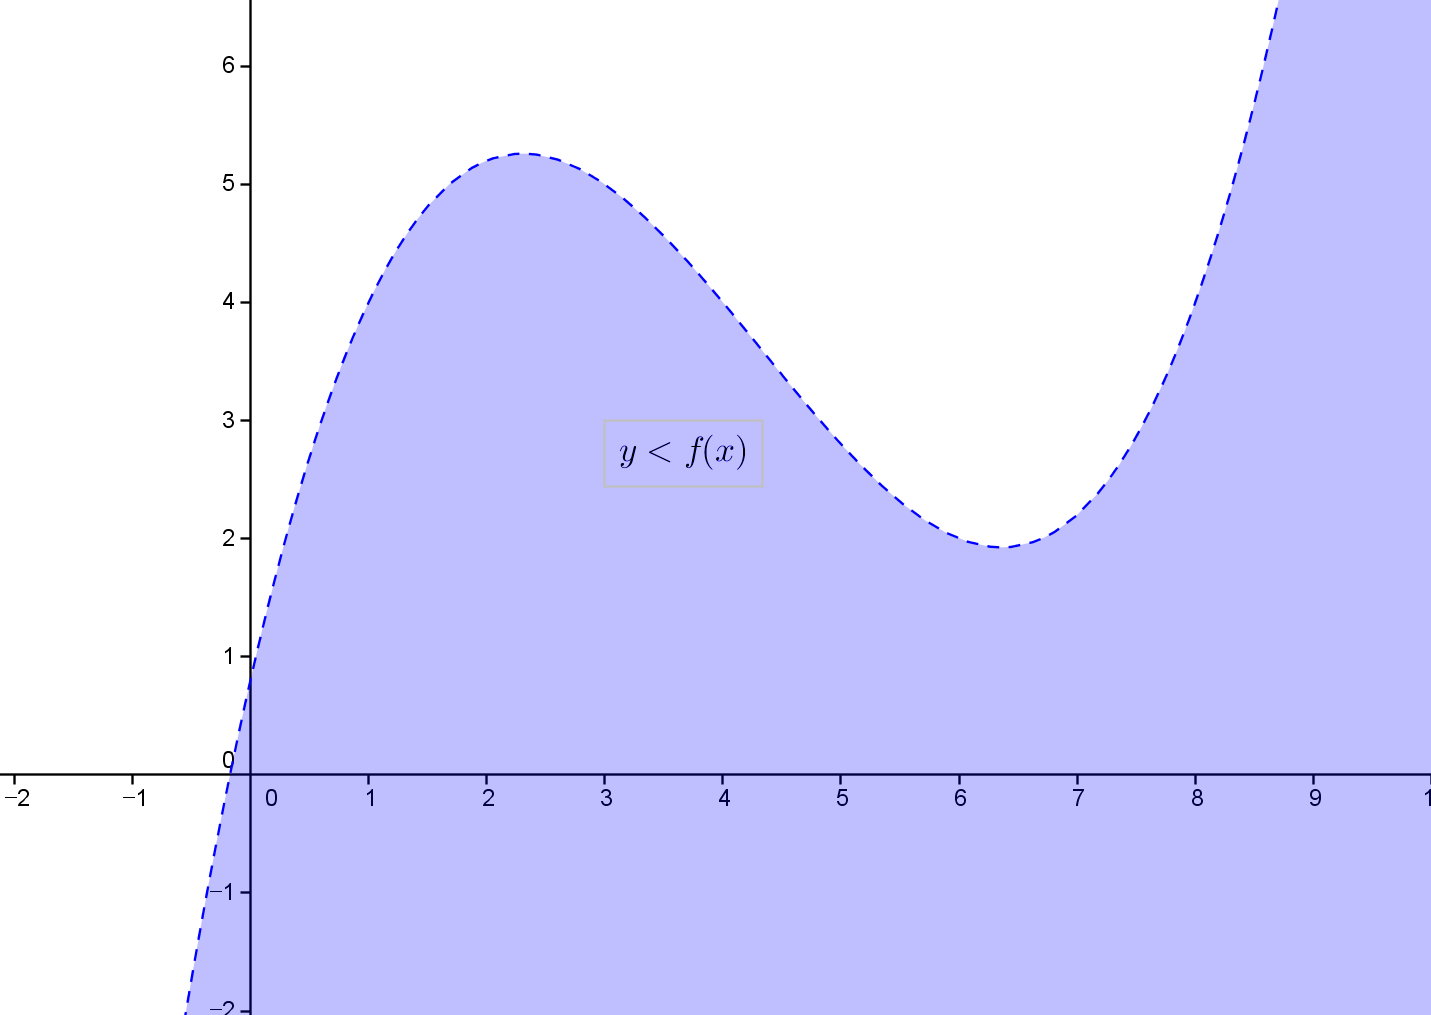
\includegraphics[width=0.24\textwidth]{ineq_3}}
&\raisebox{-.5\height}{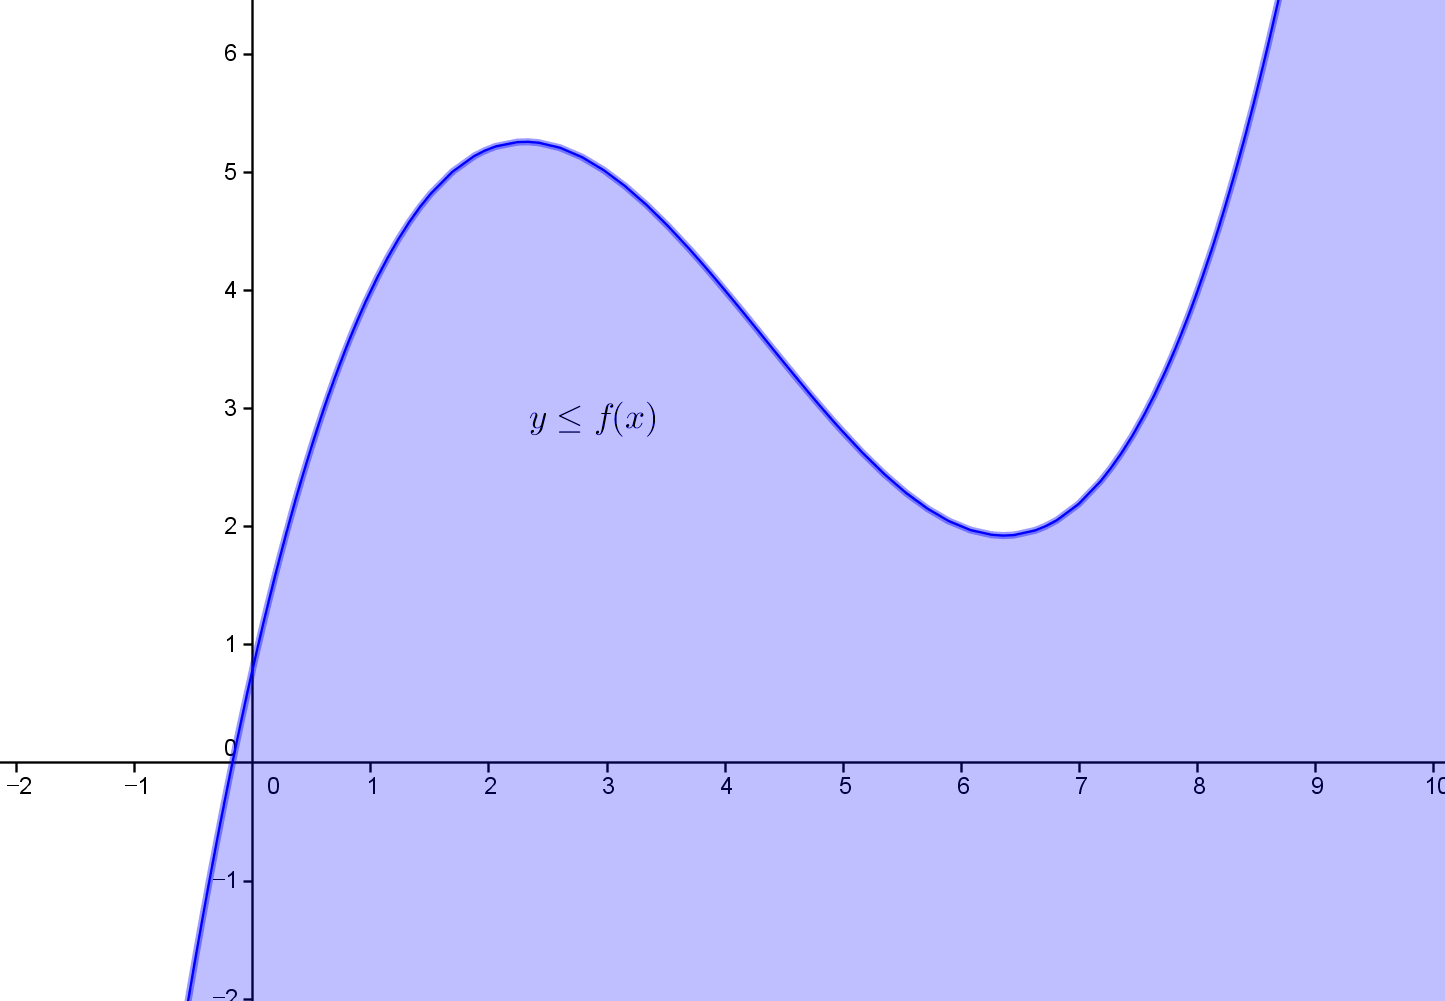
\includegraphics[width=0.24\textwidth]{ineq_4}}
\\\hline
\end{tabular}}
\item
경계선이 원인 경우의 부등식의 영역은 다음과 같이 표시된다.
\par
\bigskip
\noindent
{\footnotesize
\begin{tabular}{p{0.24\textwidth}|p{0.24\textwidth}|p{0.24\textwidth}|p{0.24\textwidth}}
\hline
\(x^2+y^2<r^2\)	&\(x^2+y^2\le r^2\)	&\(x^2+y^2>r^2\)	&\(x^2+y^2\ge r^2\)\\
\hline
\raisebox{-.5\height}{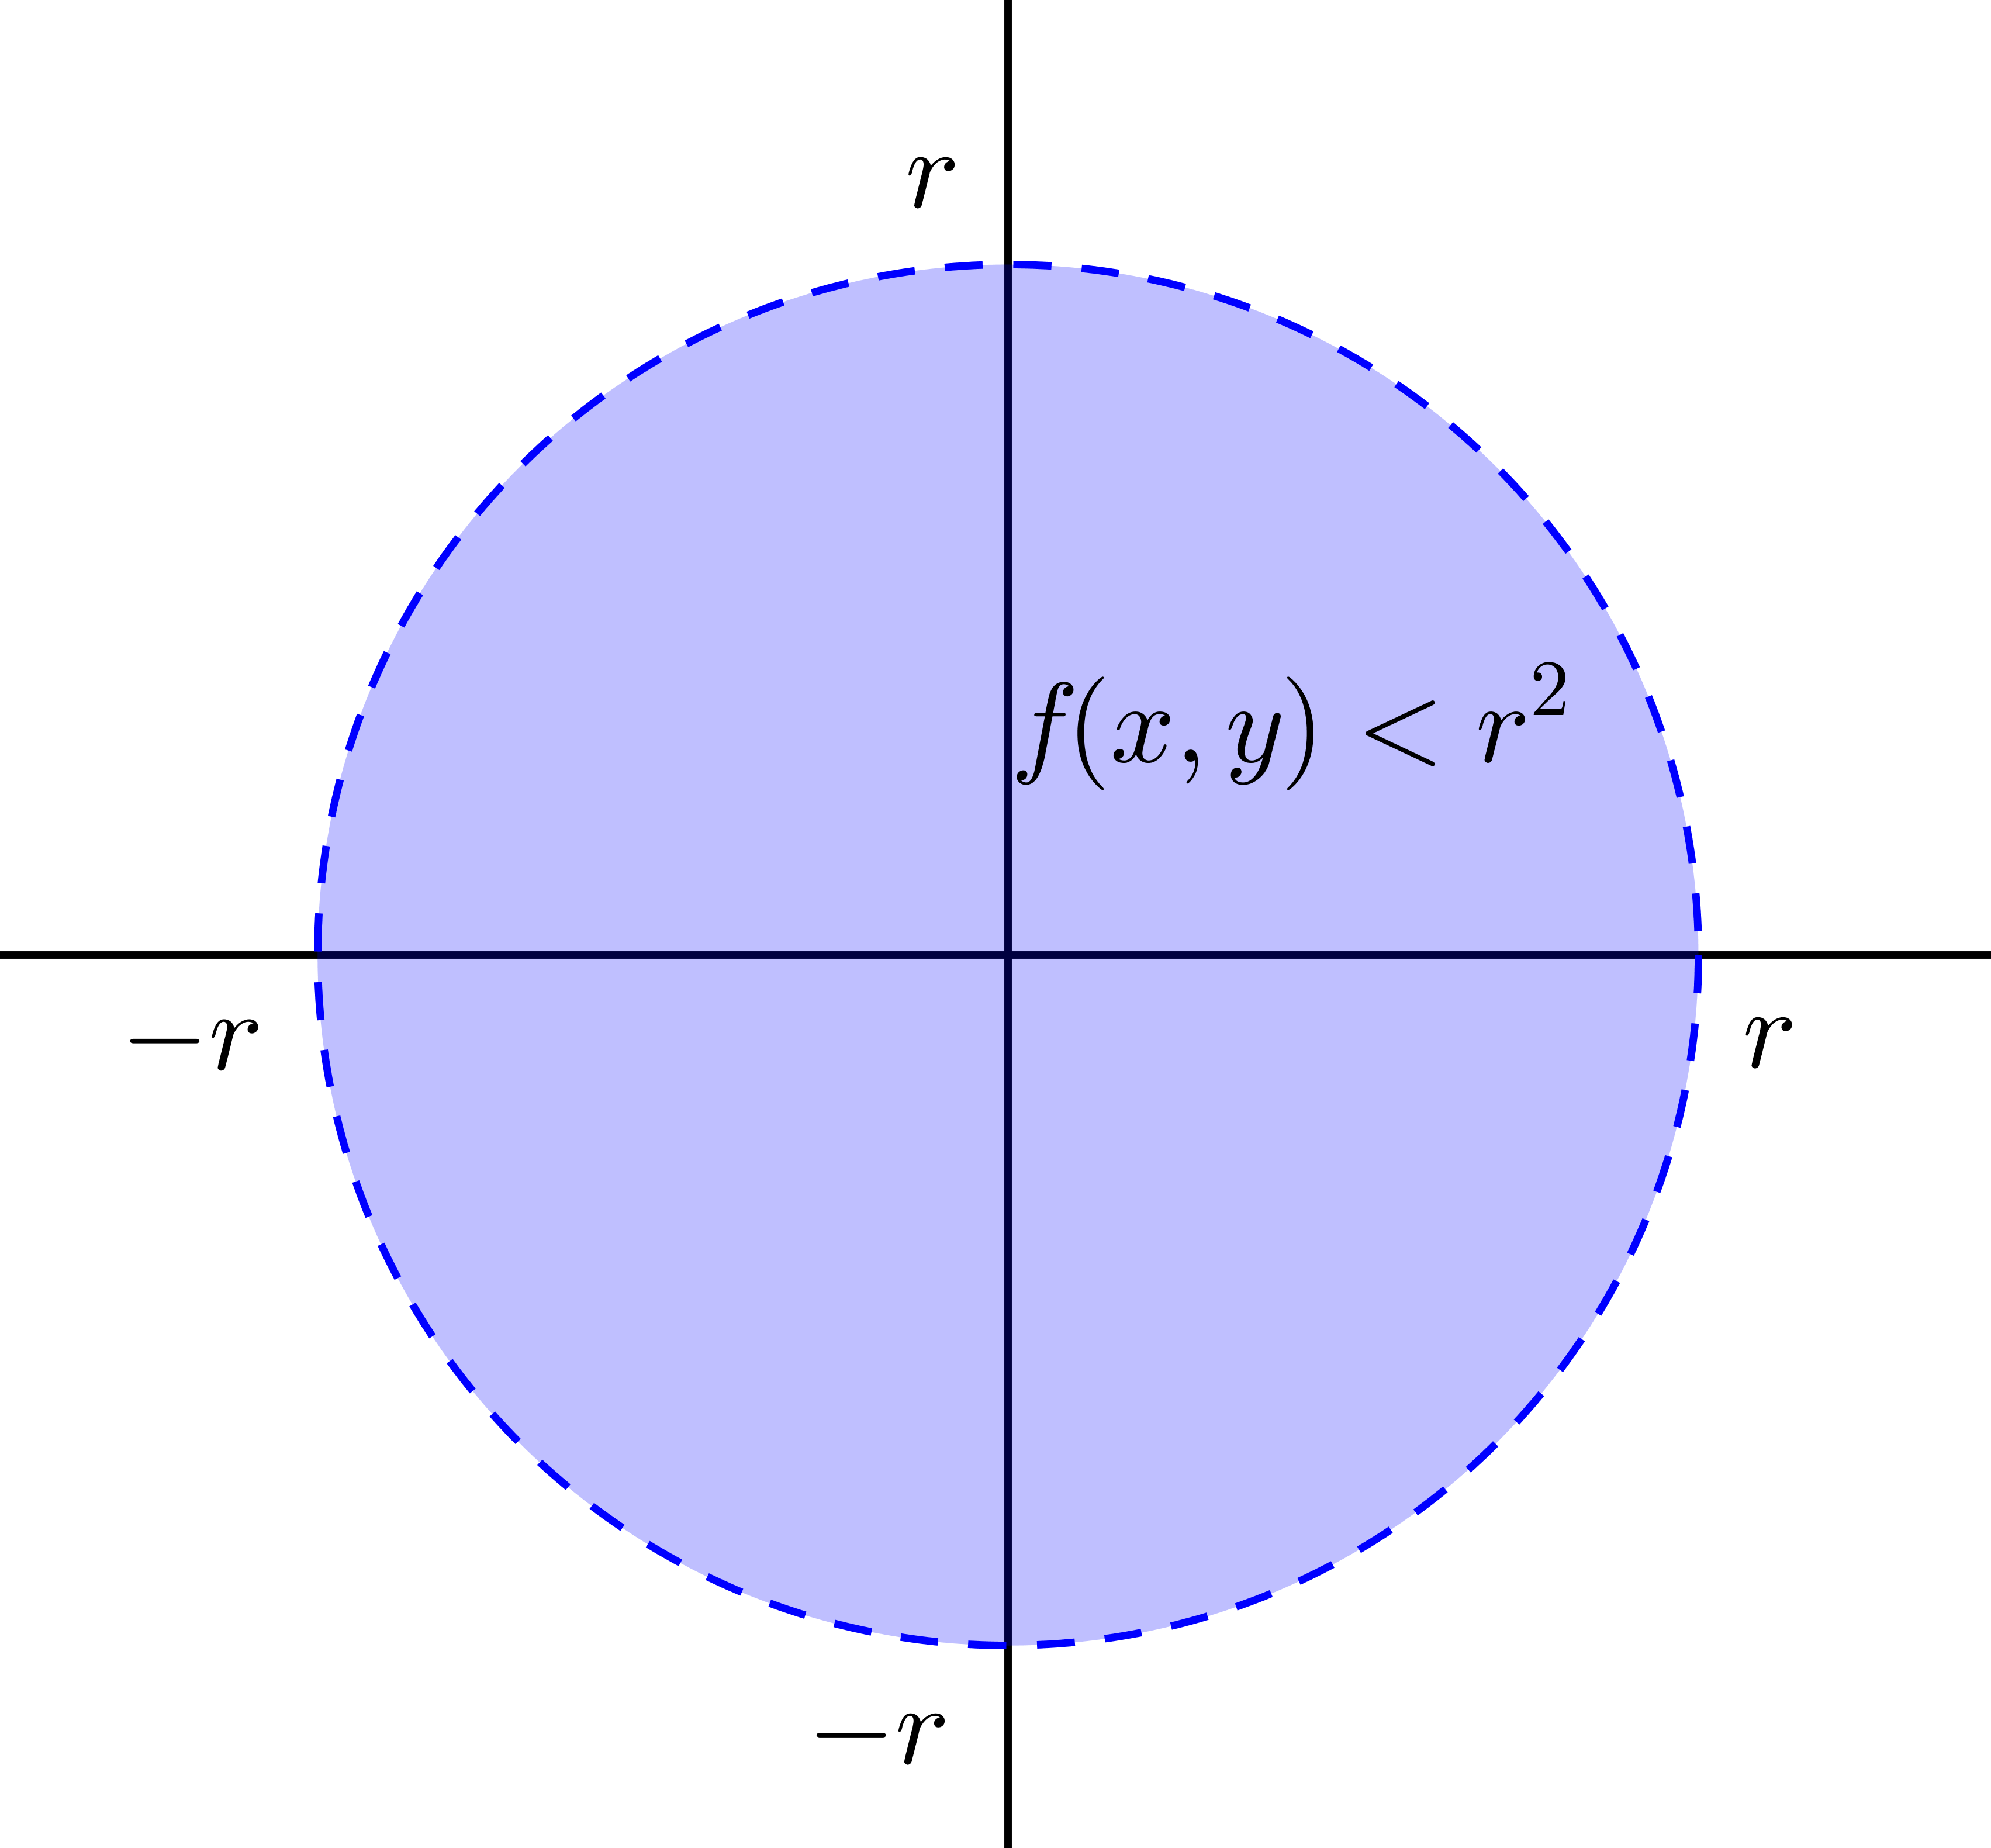
\includegraphics[width=0.24\textwidth]{ineq_circ_1}}
&\raisebox{-.5\height}{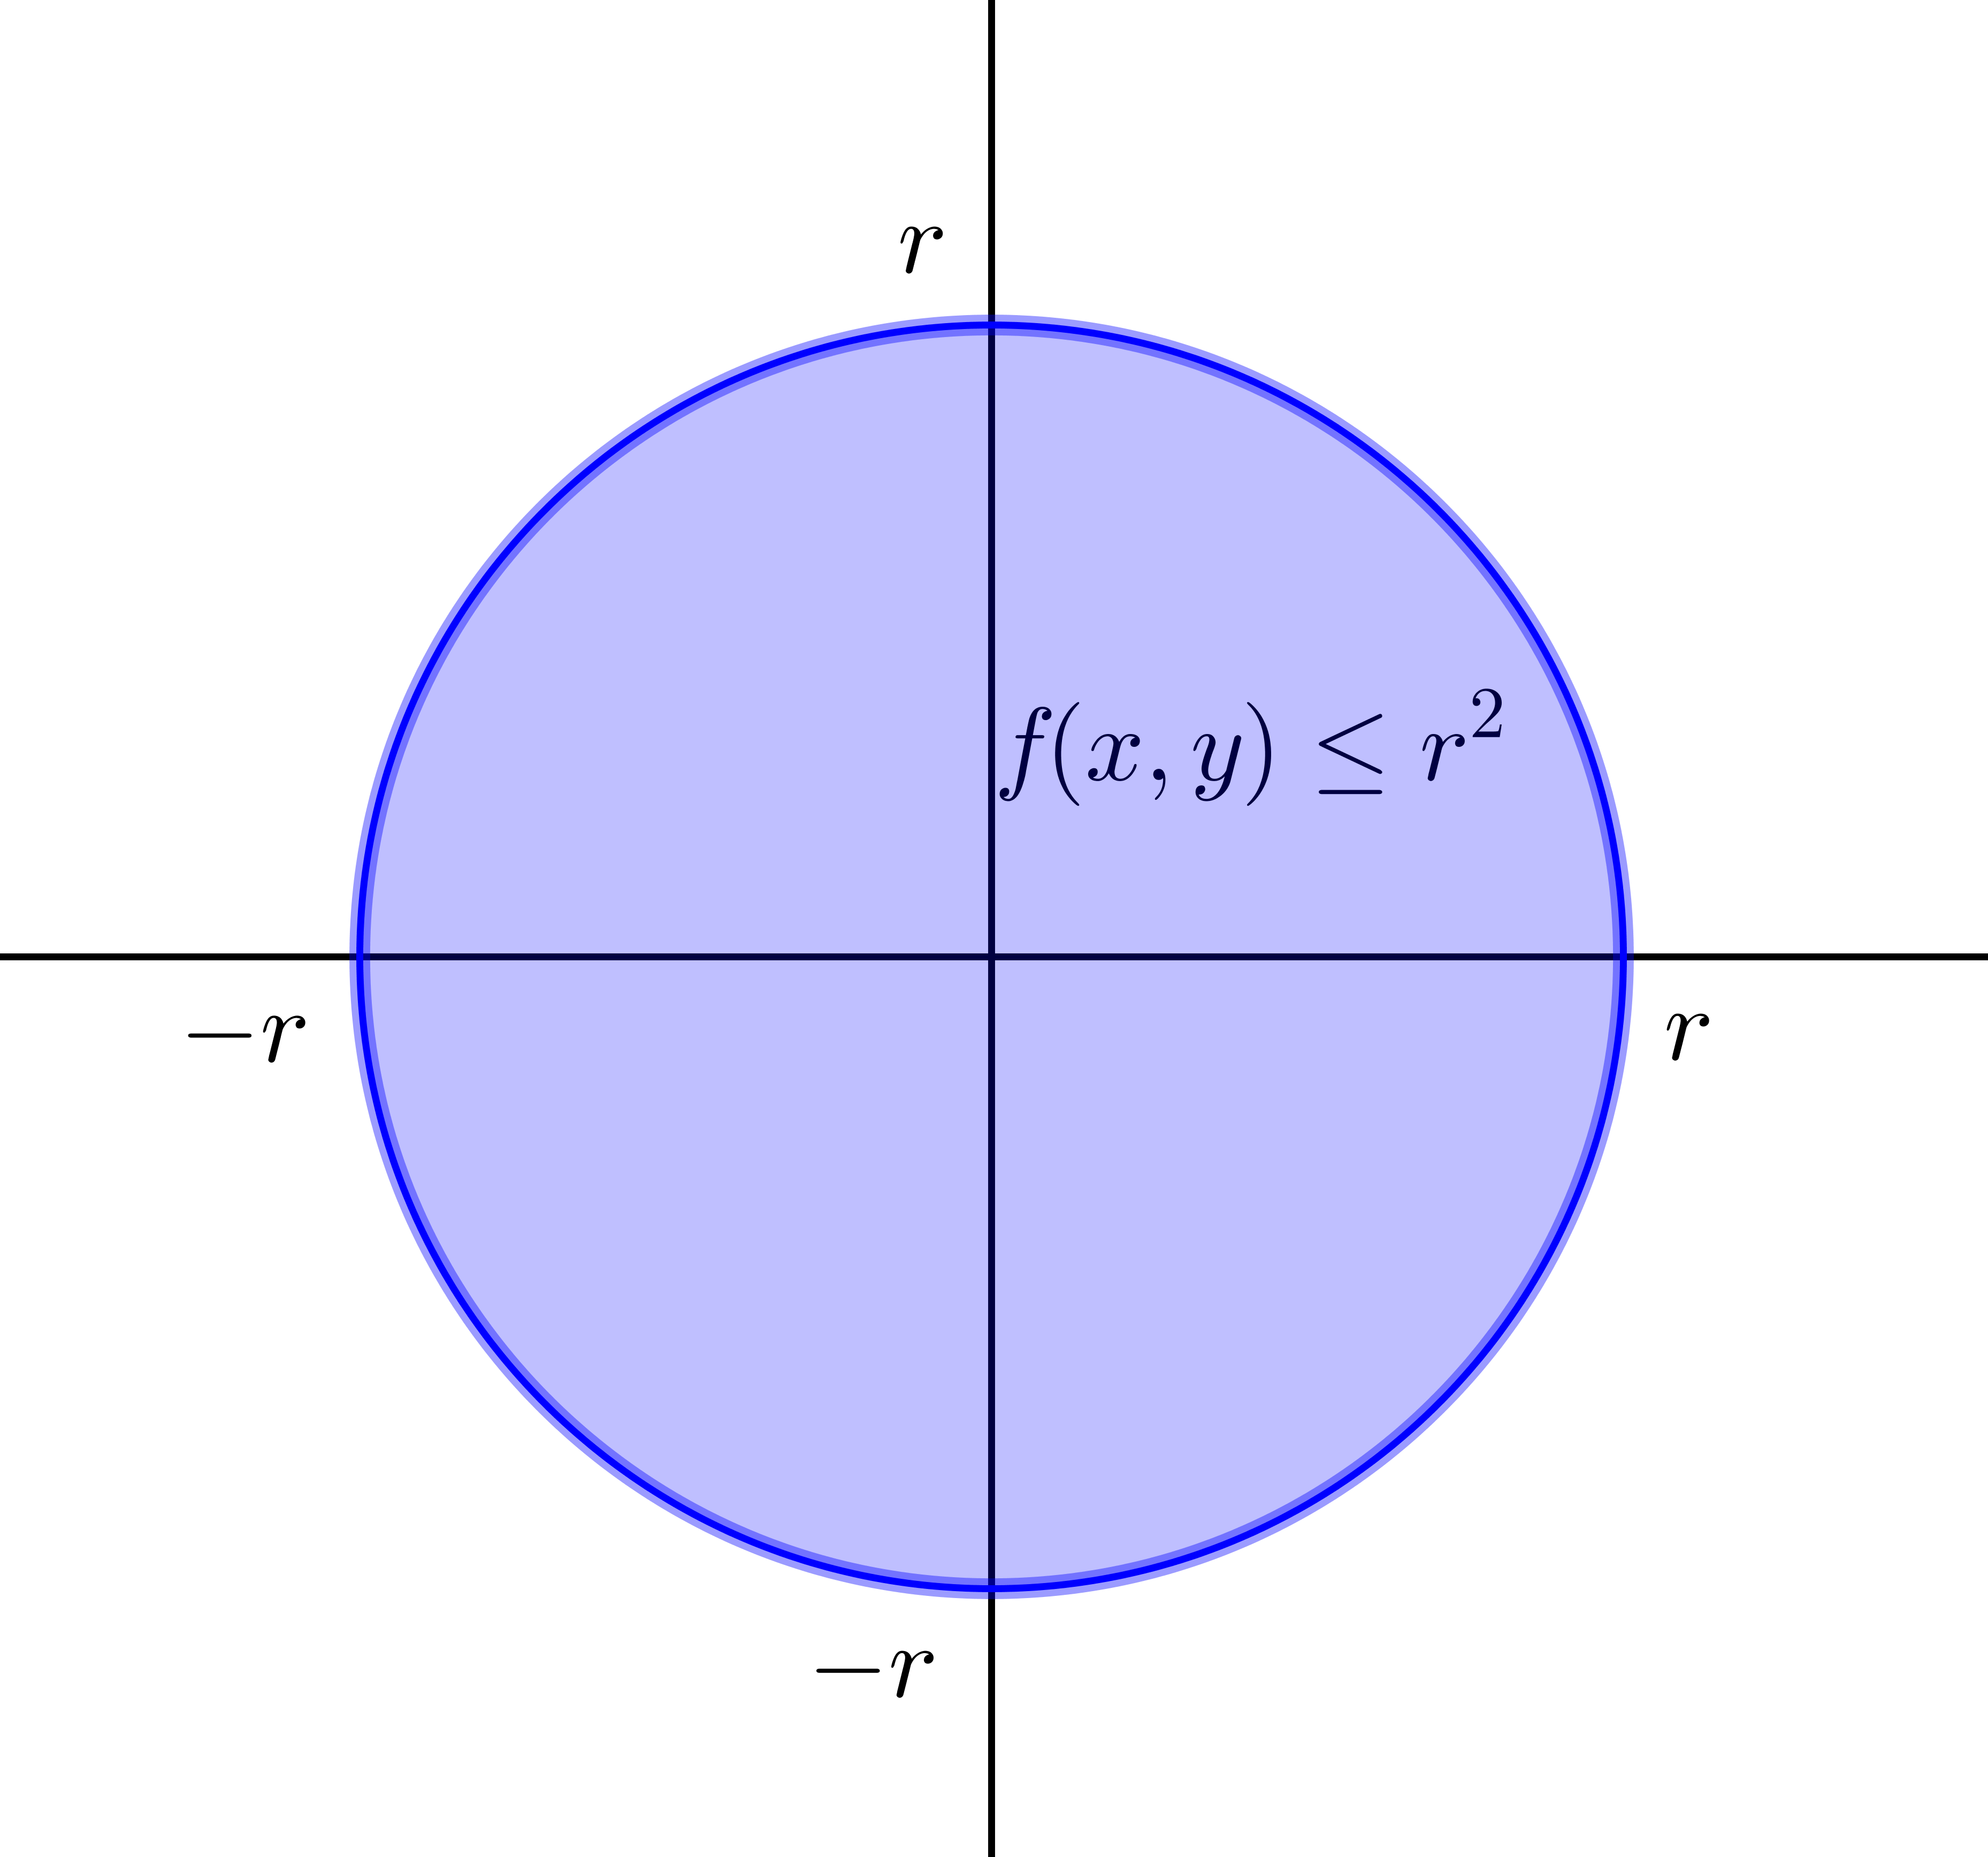
\includegraphics[width=0.24\textwidth]{ineq_circ_2}}
&\raisebox{-.5\height}{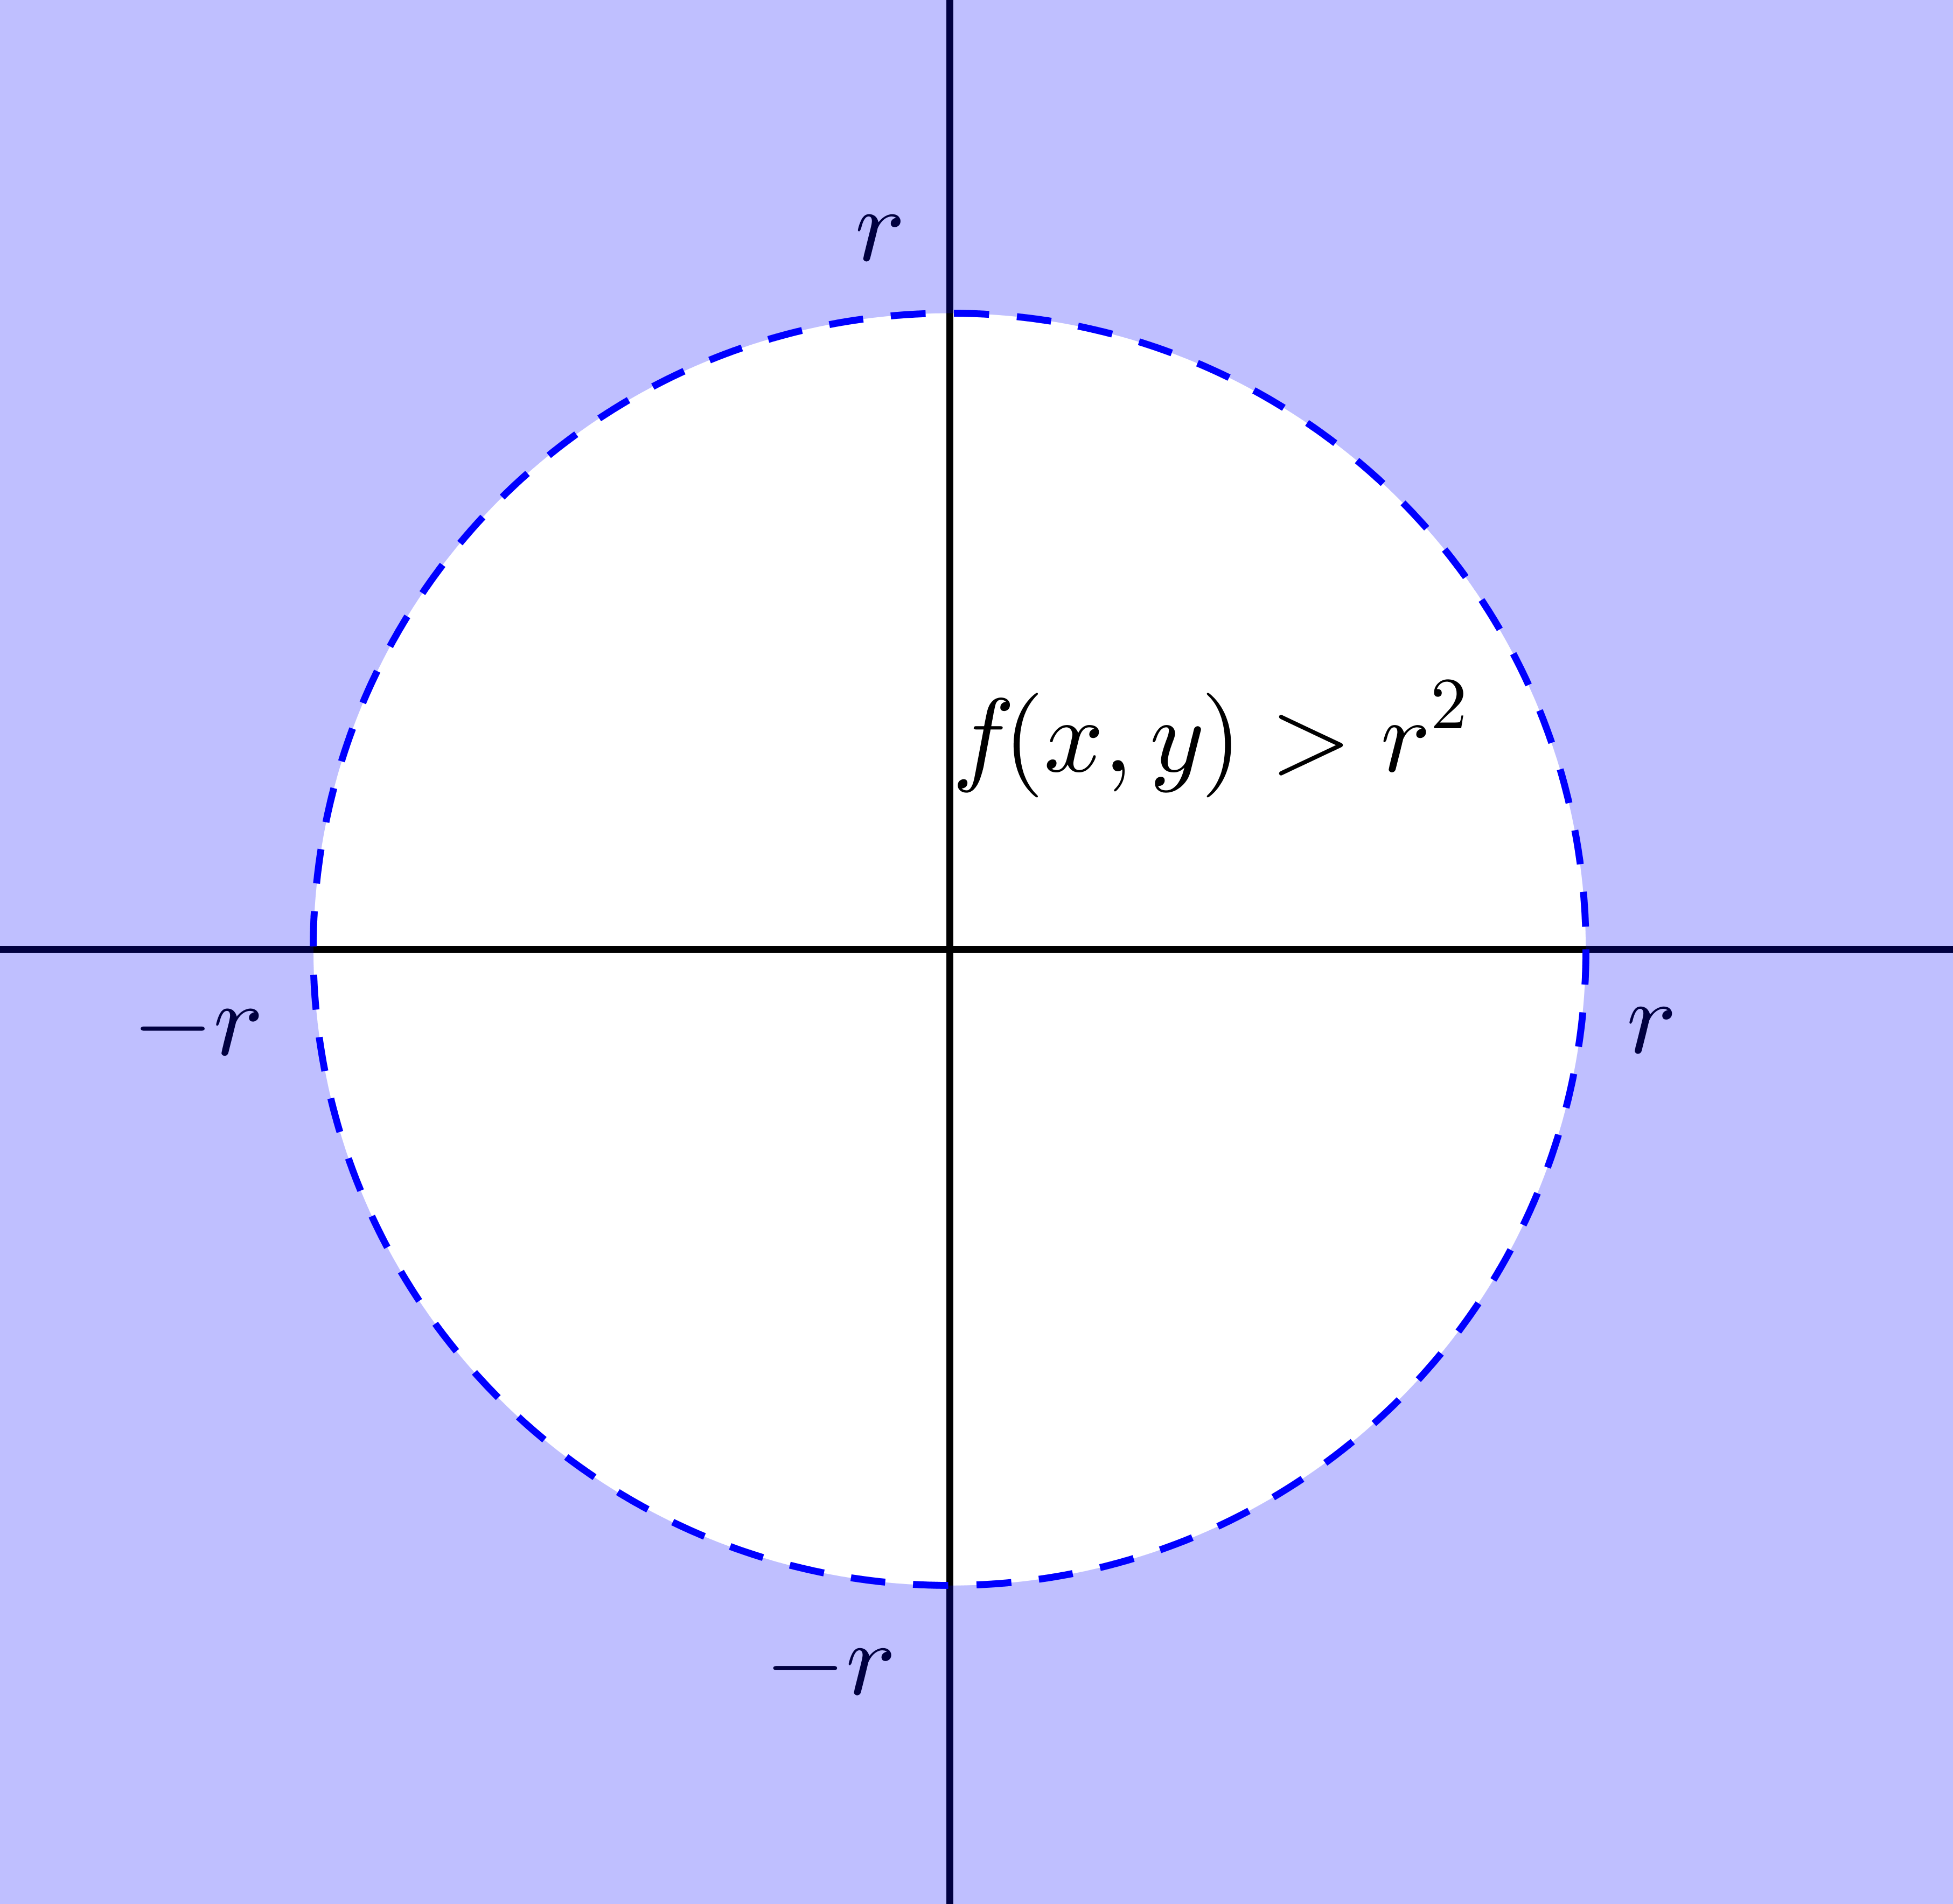
\includegraphics[width=0.24\textwidth]{ineq_circ_3}}
&\raisebox{-.5\height}{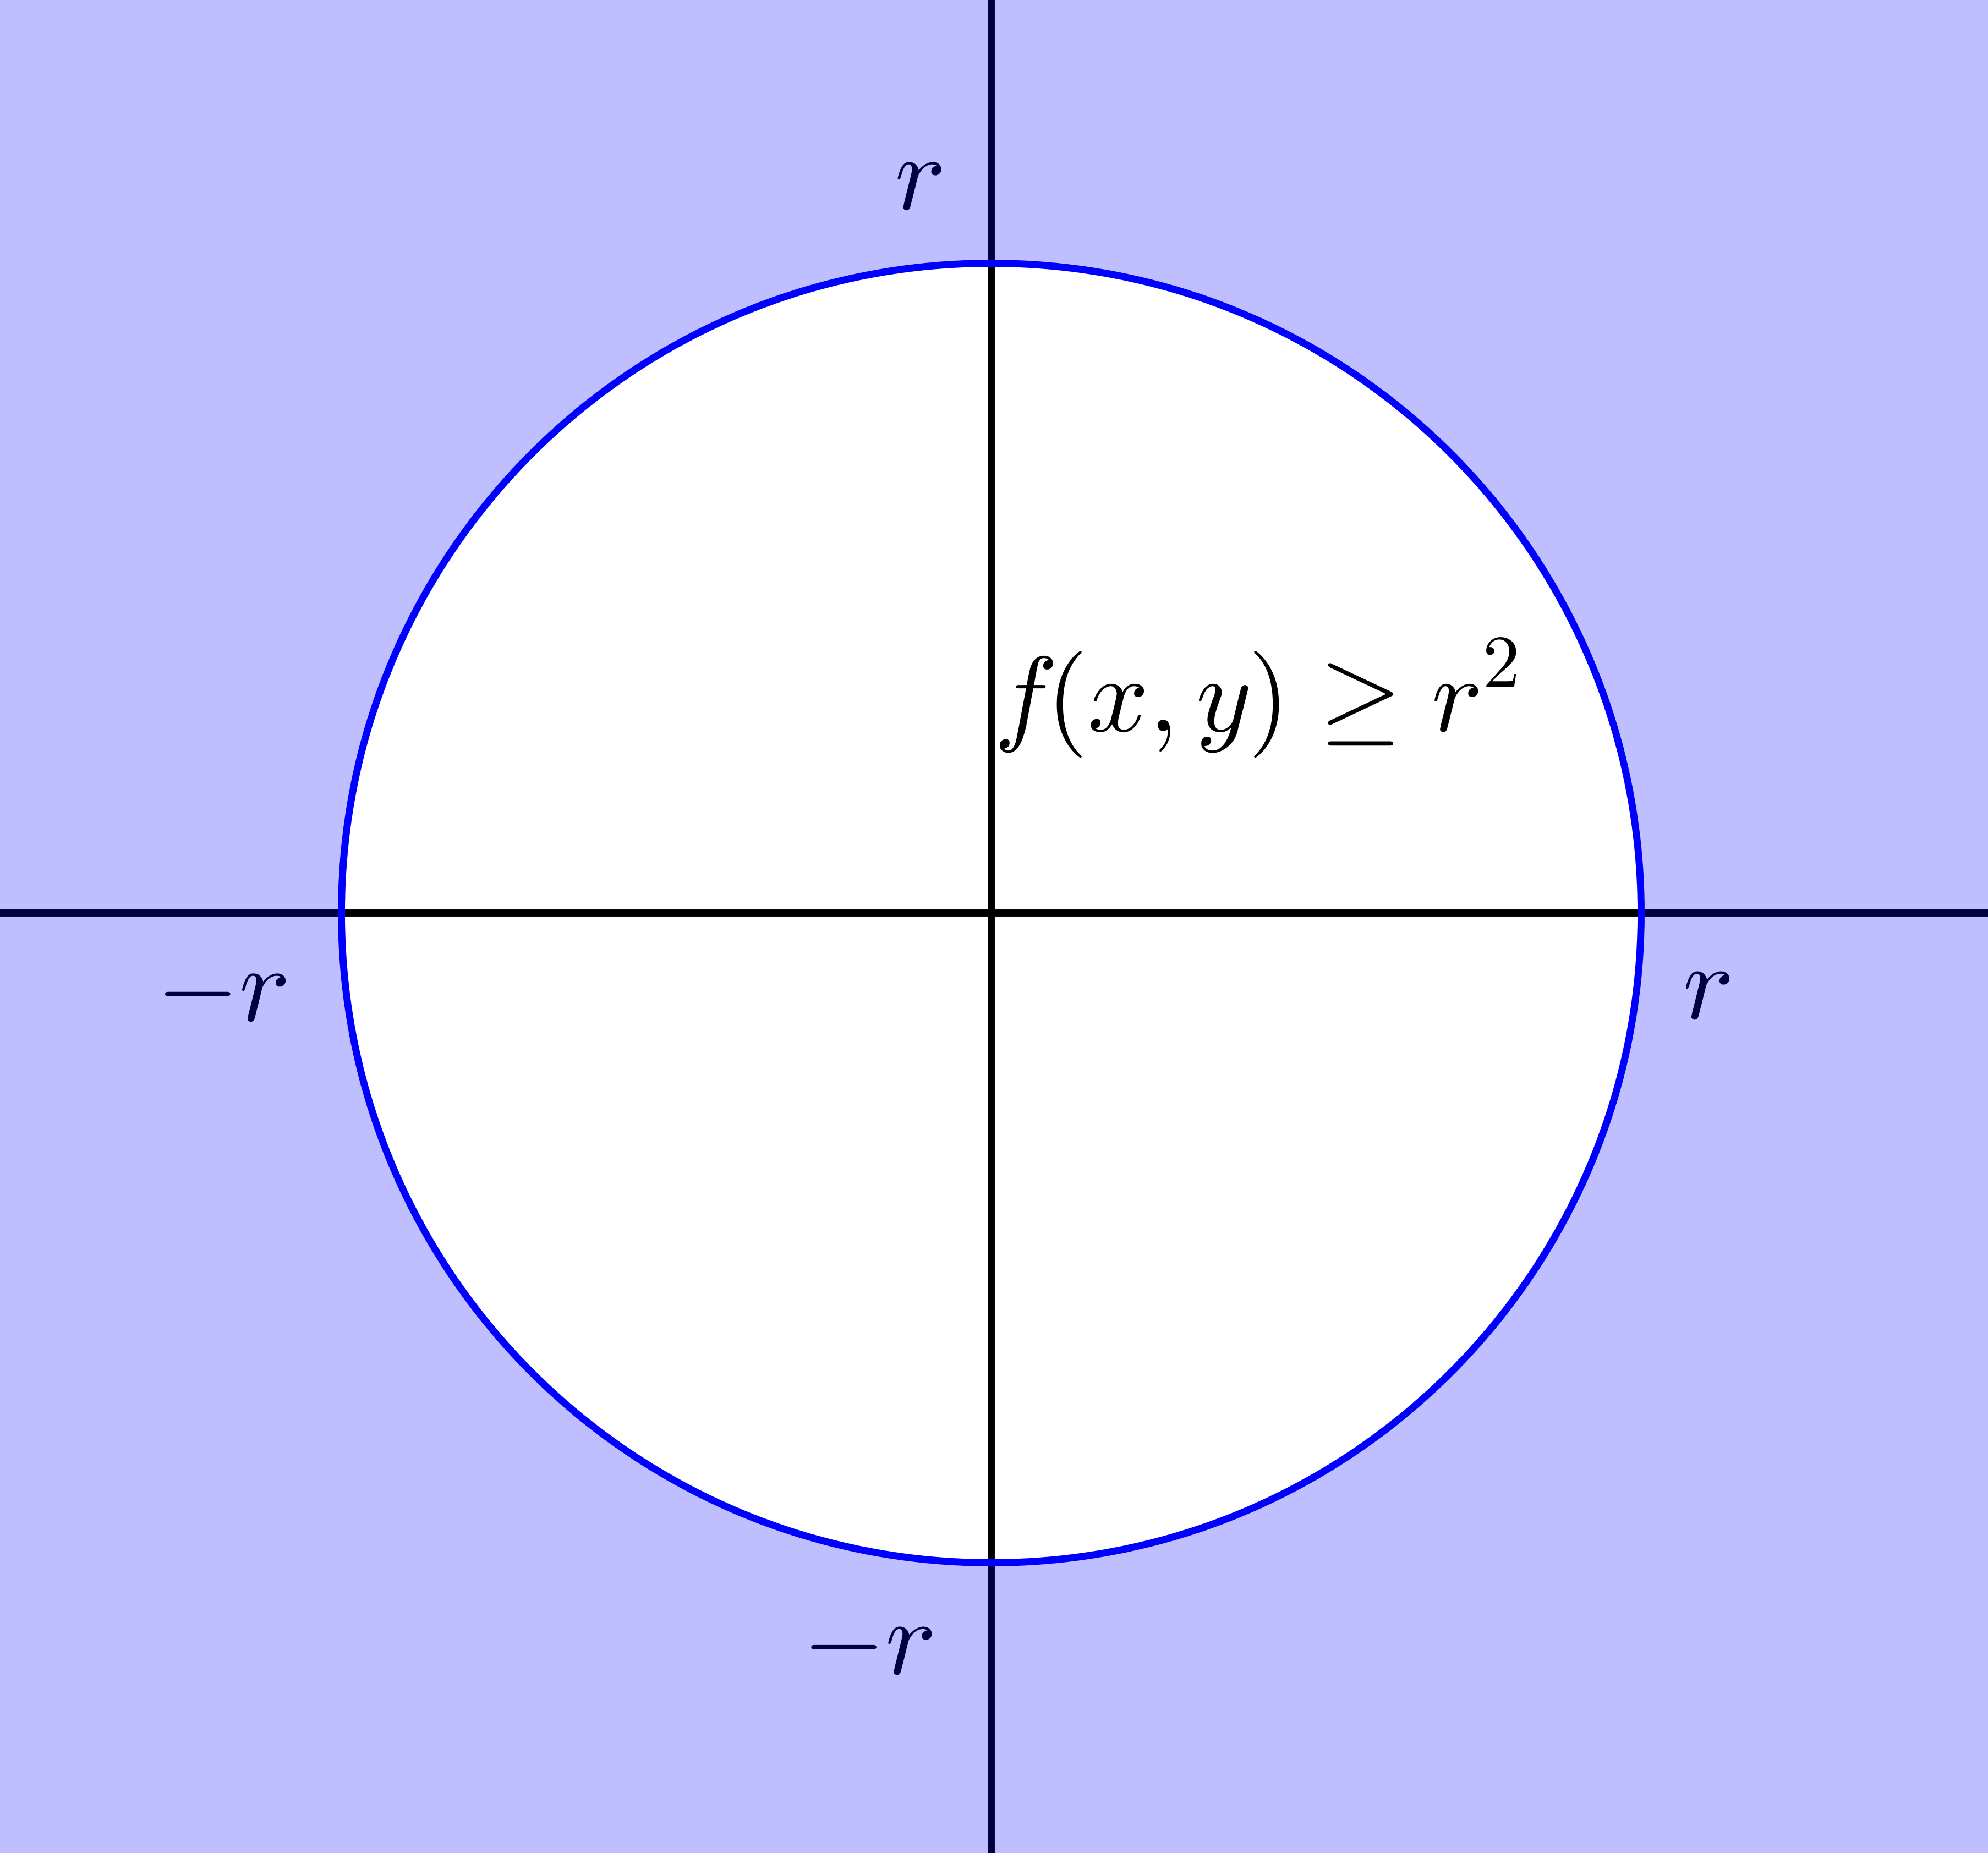
\includegraphics[width=0.24\textwidth]{ineq_circ_4}}
\\\hline
\end{tabular}}
\item
연립 부등식의 경우, 두 부등식의 영역이 겹쳐지는 부분이 연립 부등식의 영역이다.
\end{enumerate}

%
\exam{}
다음 연립부등식의 영역을 좌표평면 위에 나타내어라.
\[
\begin{cases}
y<x+2\\
x^2+y^2<9
\end{cases}
\]

\sol
첫 번째 부등식을 나타내면

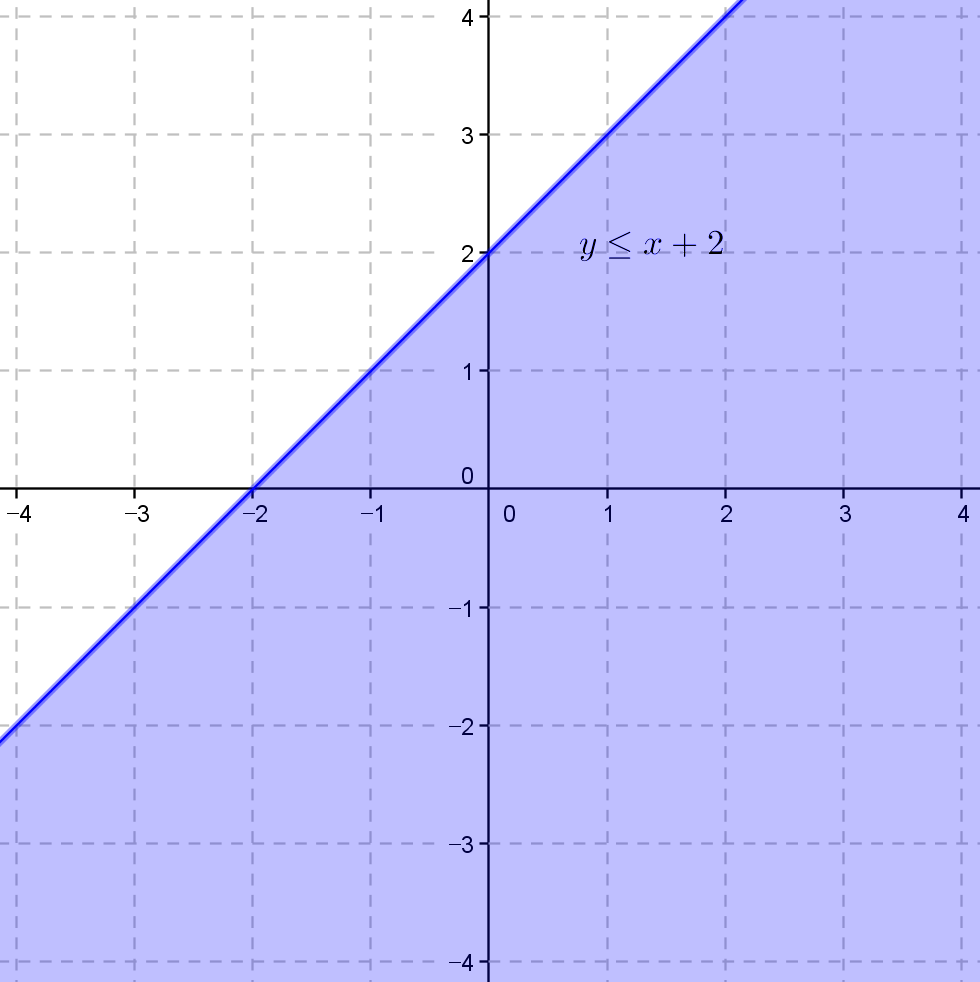
\includegraphics[width=0.3\textwidth]{range-1-1}

이고, 두 번째 부등식을 나타내면

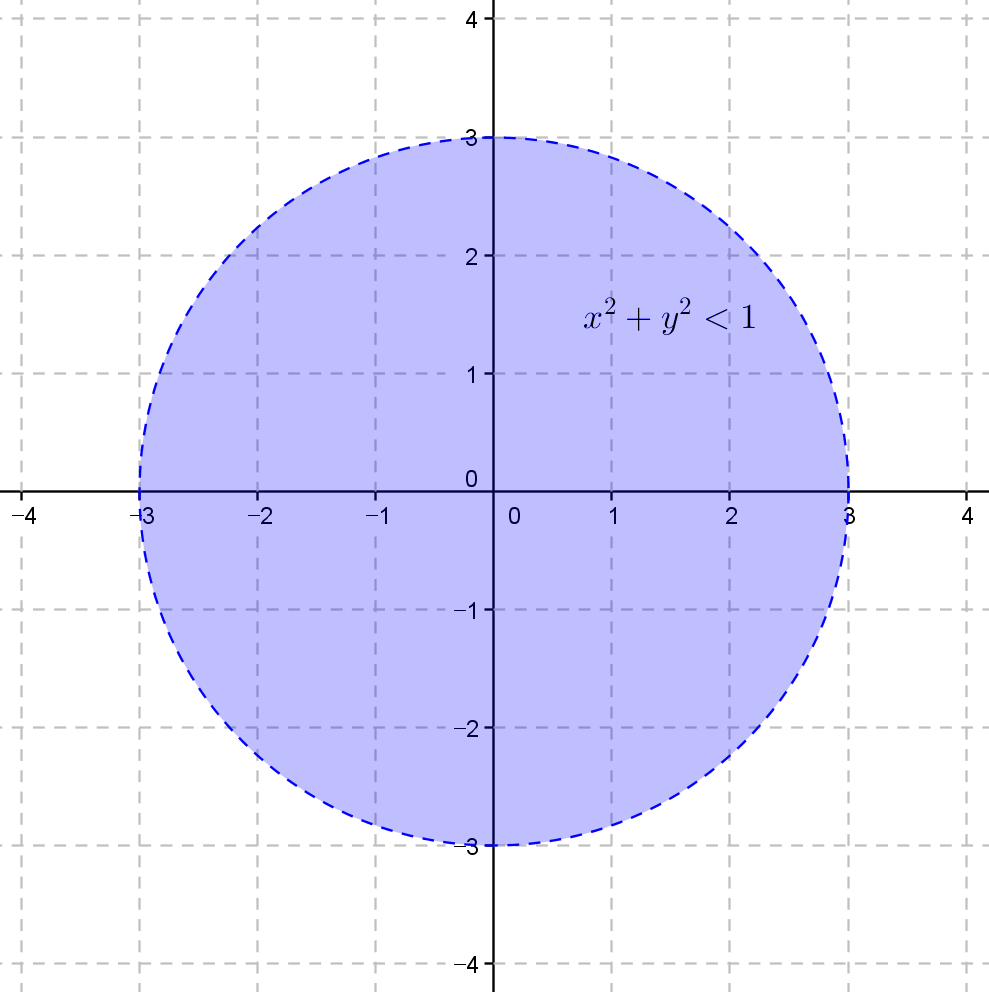
\includegraphics[width=0.3\textwidth]{range-1-2}

이므로 두 영역의 공통부분인

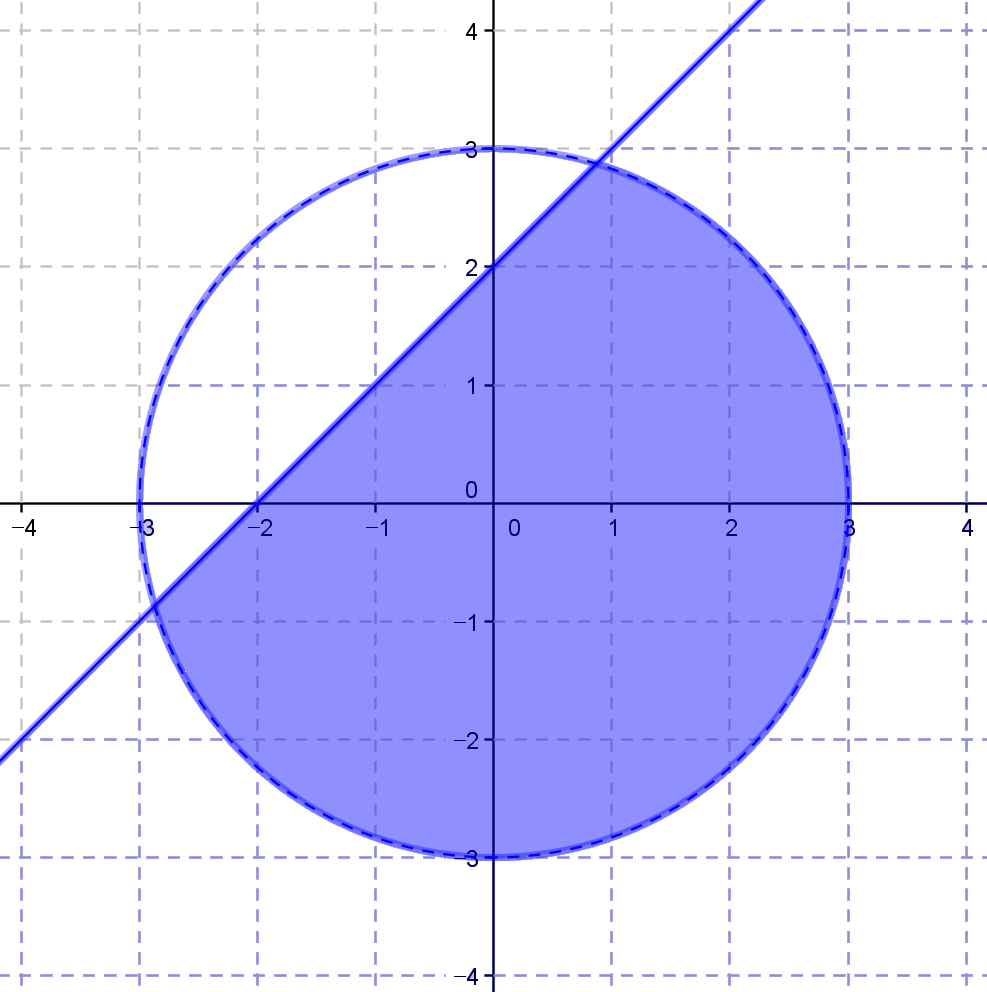
\includegraphics[width=0.3\textwidth]{range-1-3}

가 답이 된다.

%
\prob{}
다음 연립 부등식의 영역을 좌표평면 위에 나타내어라.\\
(1)
\(
\begin{cases}
y>x-1\\
x^2+y^2-2x-3>0
\end{cases}
\)\\
(2)
\(x-1\le 2x+y-4\le5x+2\)

\ans{
(1)
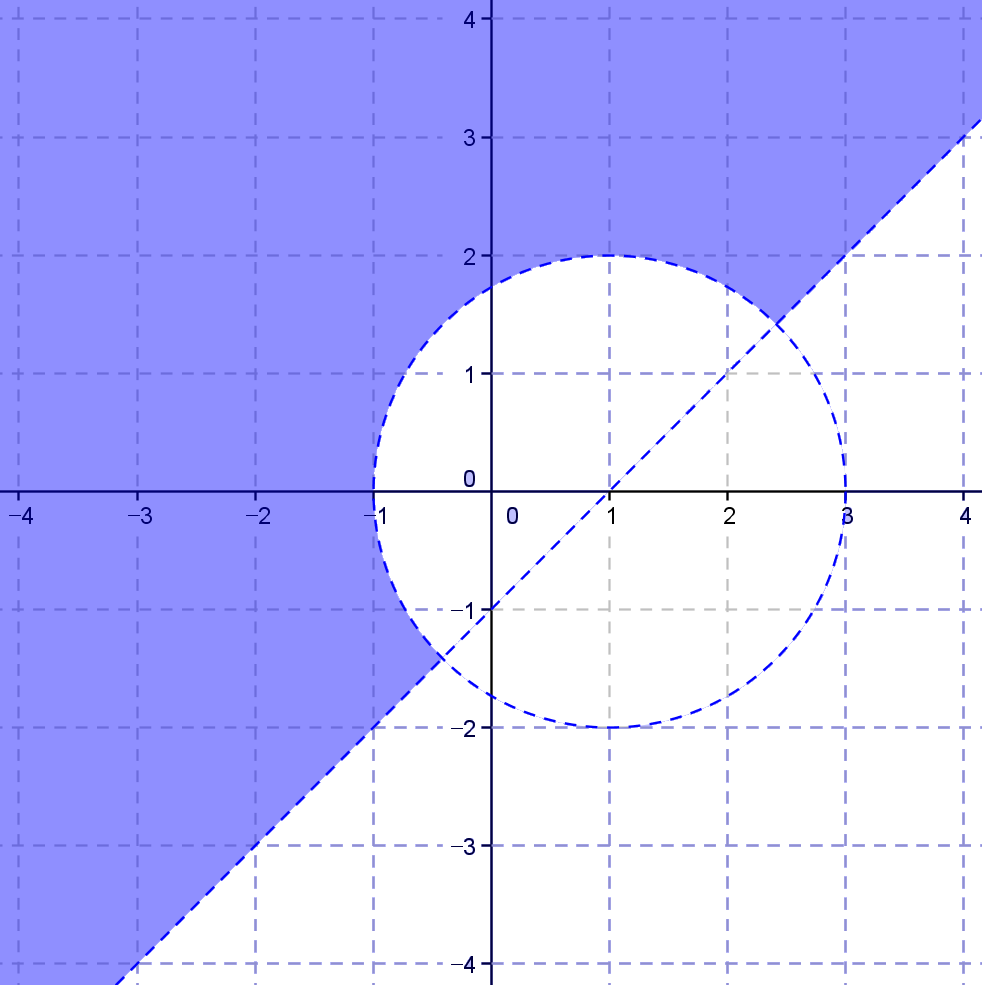
\includegraphics[width=0.2\textwidth]{range-1-4}

(2)
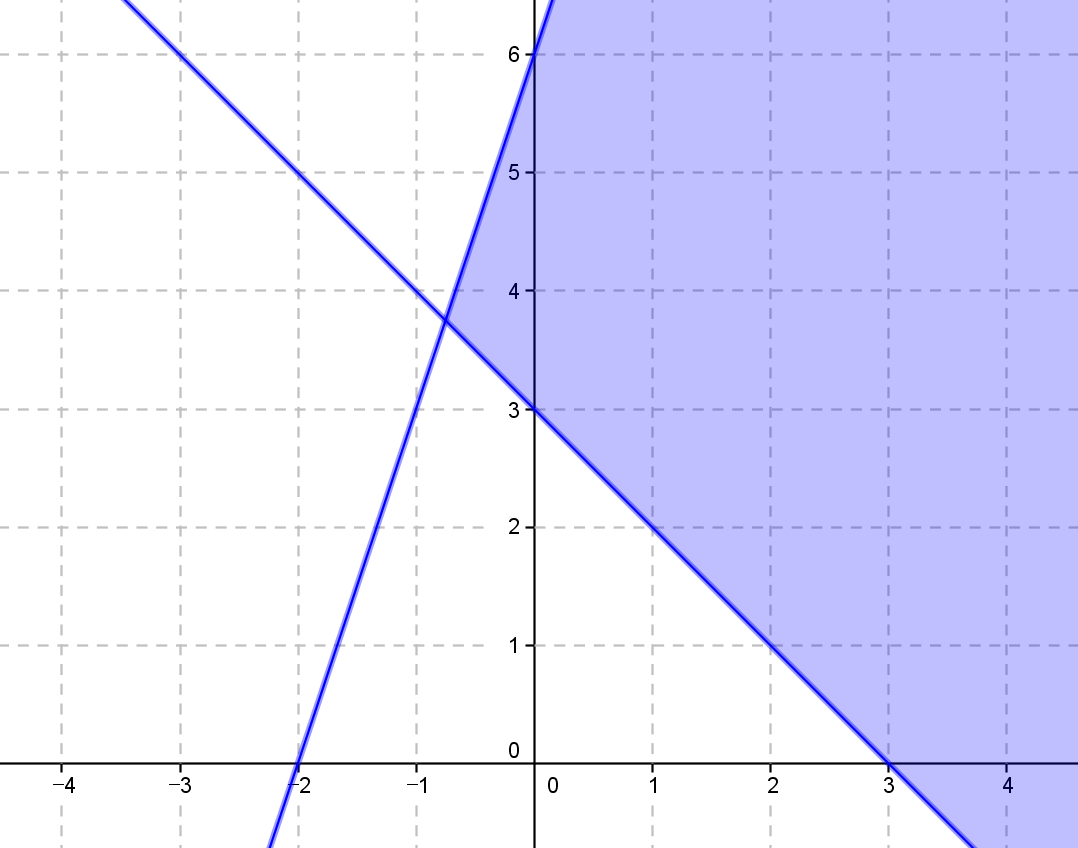
\includegraphics[width=0.2\textwidth]{range-1-5}
}

%
\exam{}
다음 부등식의 영역을 좌표평면 위에 나타내어라.\\
\[(x+y+4)(x^2+y^2+8x)<0\]

\sol
\(AB<0\)이면 \(\begin{cases}A>0\\B<0\end{cases}\)이거나 \(\begin{cases}A<0\\B>0\end{cases}\)이다.

따라서 구하는 영역은 두 연립부등식
\[
\begin{cases}x+y+4>0\\x^2+y^2+8x<0\end{cases}
\text{ 또는 }
\begin{cases}x+y+4<0\\x^2+y^2+8x>0\end{cases}
\]
의 영역이다.
그러므로

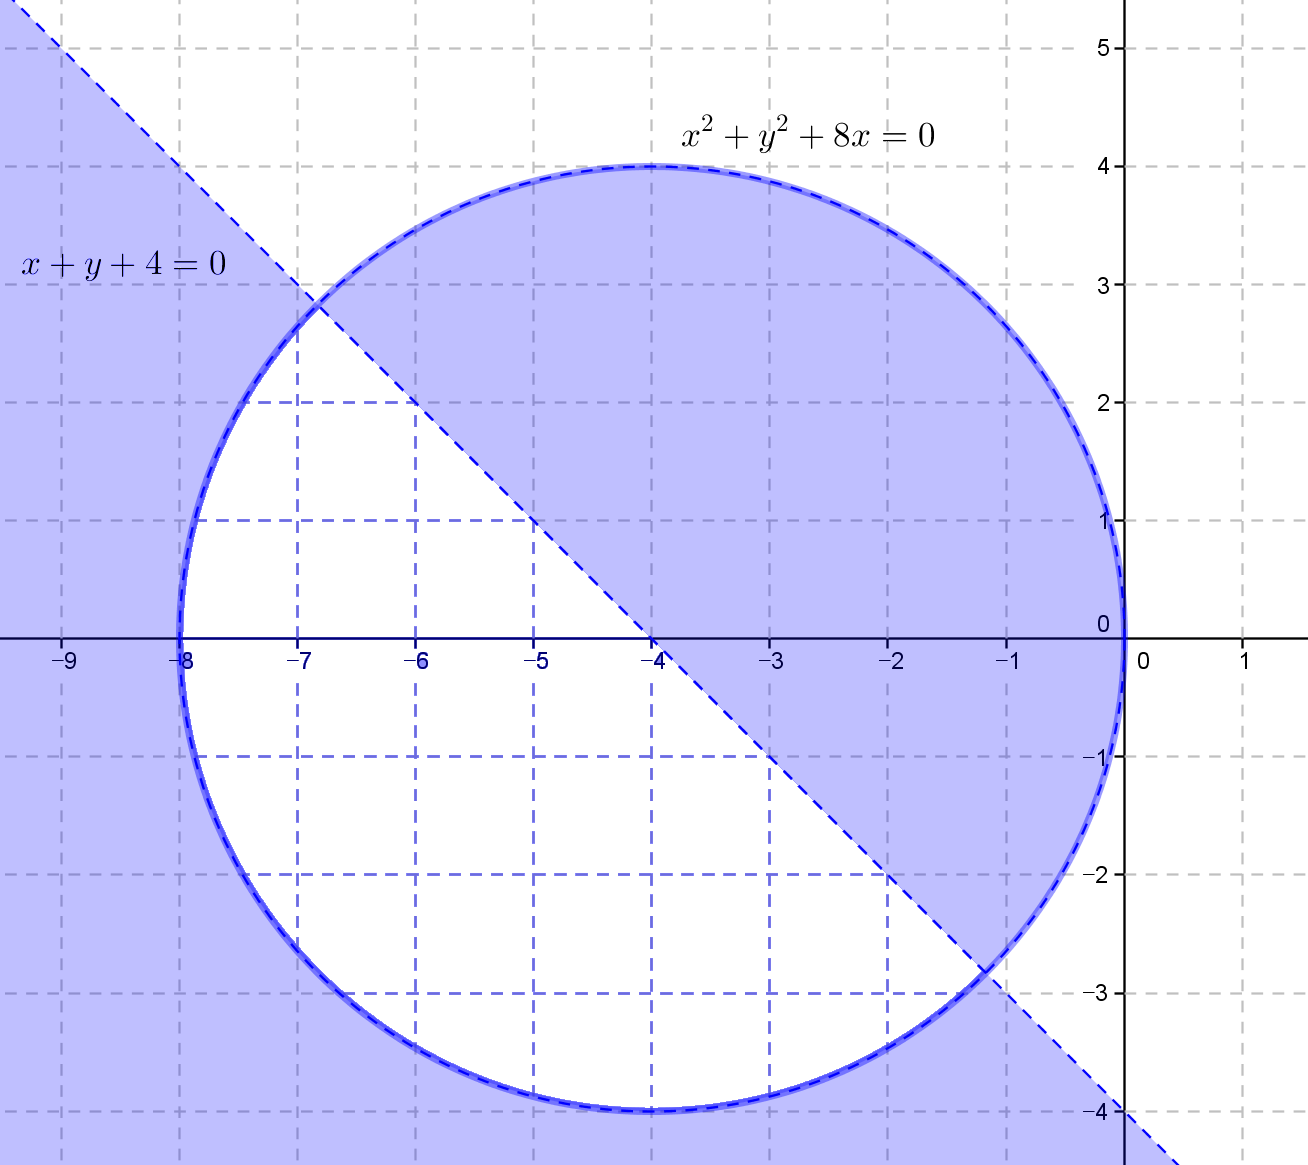
\includegraphics[width=0.4\textwidth]{range-2-1}

이 답이 된다.

\prob{}
다음 부등식의 영역을 좌표평면 위에 나타내어라.
\[(x+y-2)(x-y-3)>0\]

\ans{
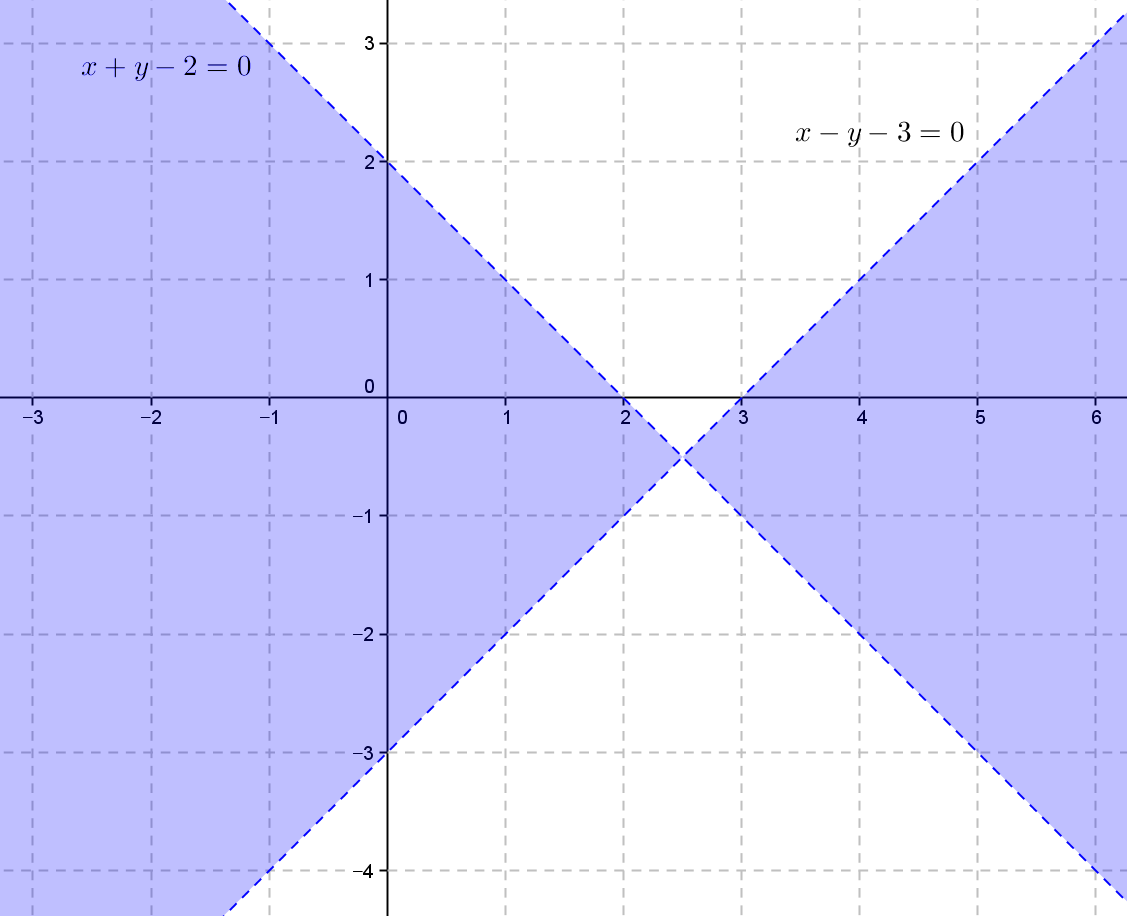
\includegraphics[width=0.2\textwidth]{range-2-2}
}

\exam{}
연립부등식 \(x\ge0\), \(y\ge0\), \(x+2y\le8\), \(2x+y\le10\)을 만족하는 \(x\), \(y\)에 대해 \(x+y\)의 최댓값을 구하여라.

\sol
주어진 부등식의 영역 \(D\)는 아래 그림과 같이 표현될 수 있다.
점 \(P(x,y)\)는 \(D\) 내부를 움직인다.
이때 \(x+y\)의 최댓값을 찾으면 된다.

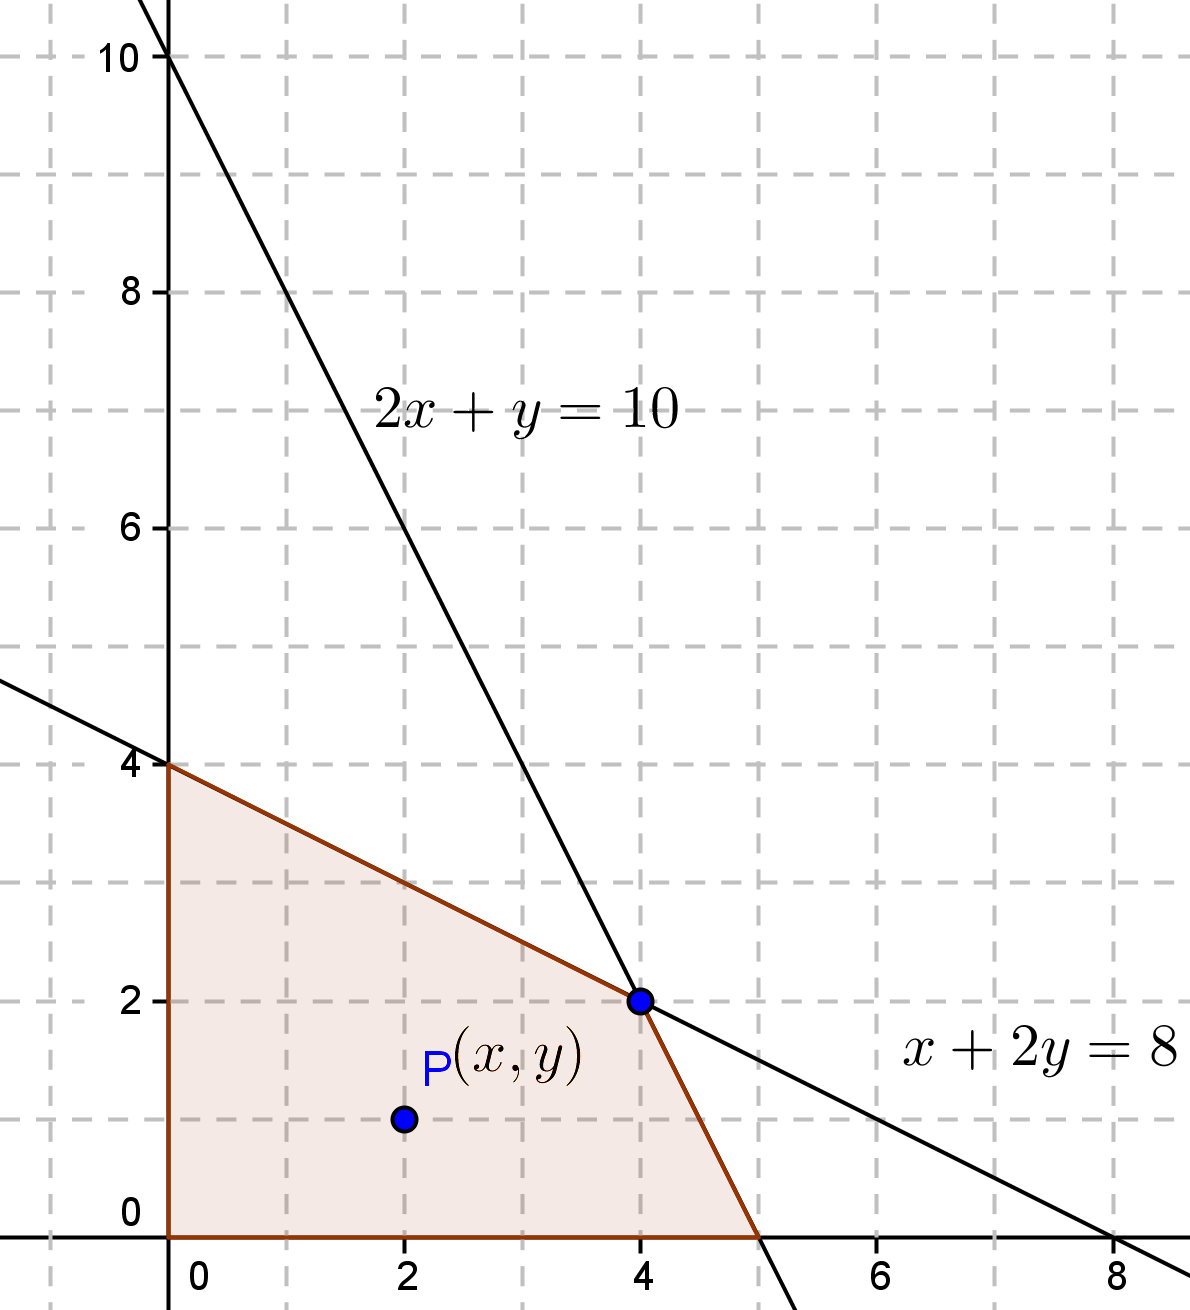
\includegraphics[width=0.4\textwidth]{range-3-1}

\(x+y\)의 값은 \(3\)일 수 있다.
왜냐하면, \(x+y=3\)이 나타내는 직선과 영역 \(D\)가 겹치기 때문이다.
겹치는 부분은 아래 그림에서 선분 \(AB\)이다.
예를 들어 \((x,y)=(0,3)\), \((1,2)\), \((2,1)\), \((3,0)\)인 경우에 \((x,y)\)는 \(D\) 안에 있고 \(x+y=3\)이다.

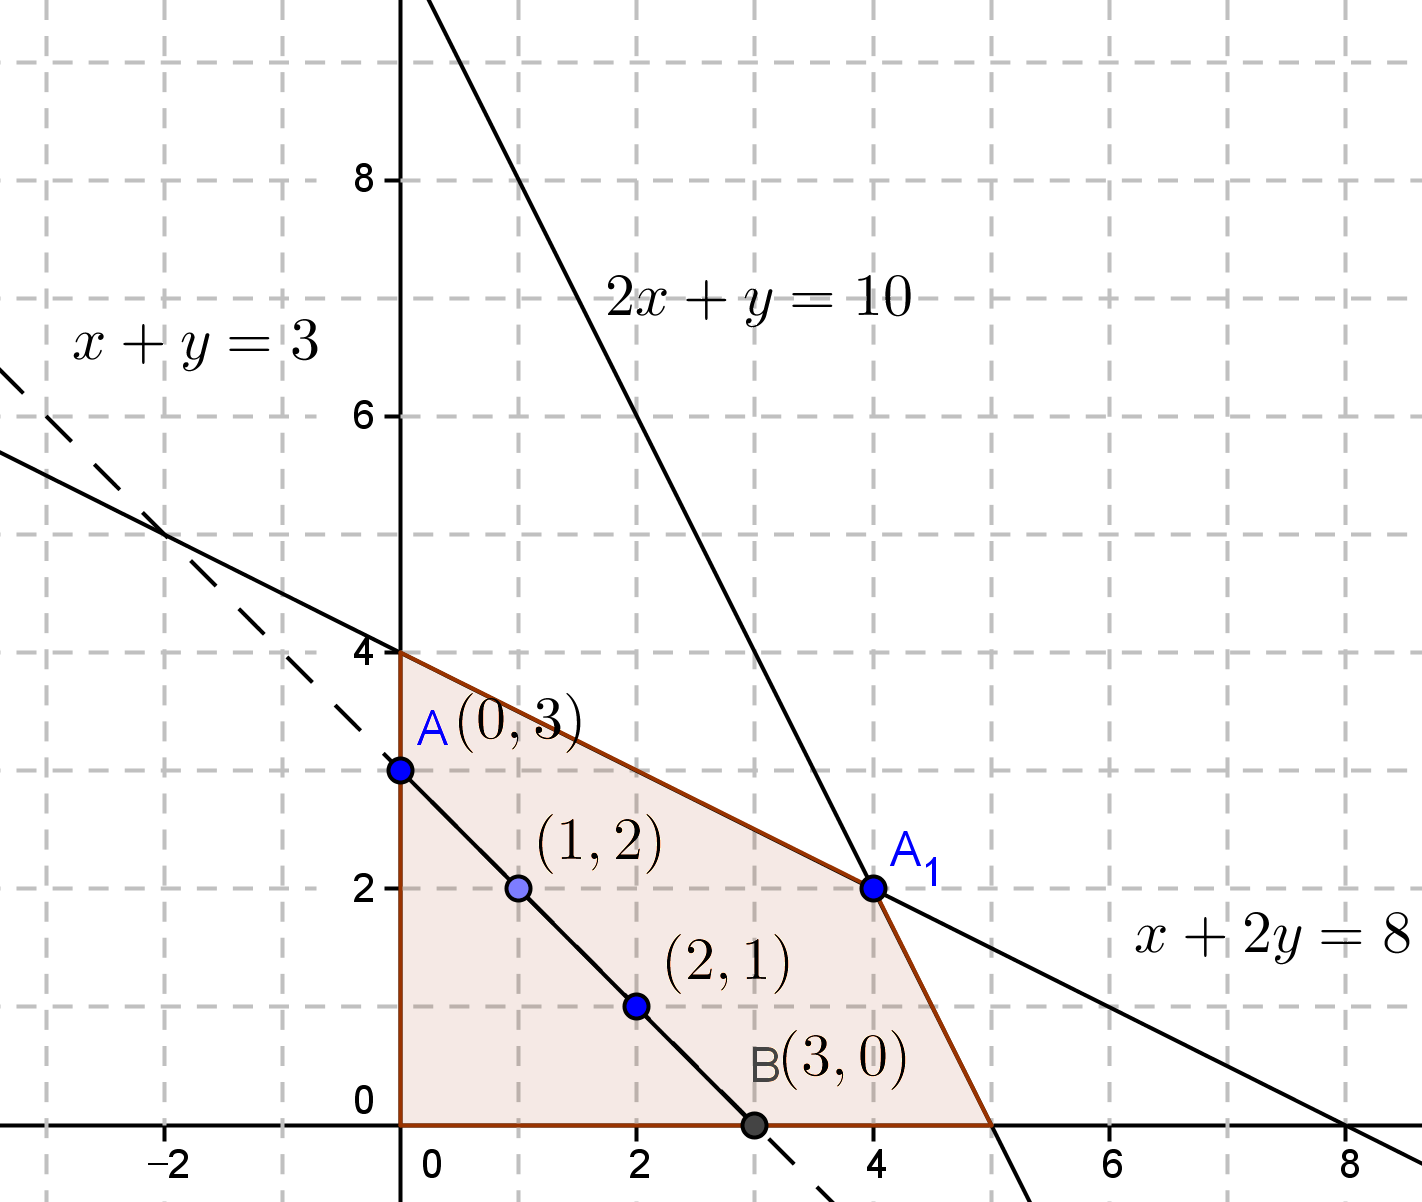
\includegraphics[width=0.4\textwidth]{range-3-2}

마찬가지의 논리로 \(x+y\)의 값은 \(4\)도 될 수 있고, \(5\)도 될 수 있다.
즉 직선 \(x+y=k\)와 영역 \(D\)가 만나는 조건 하에서의 \(k\)의 최댓값을 구하면 된다.
\(x+y=k\)를 정리하면 \(y=-x+k\)이므로 이것은 기울기가 \(-1\)이고, \(y\)절편이 \(k\)인 직선이다.
\(y=-x+k\)와 영역 \(D\)가 만나는 조건 하에 \(y=-x+k\)를 잘 움직여보면, \(y=-x+k\)가 \((4,2)\)에 닿을 때 \(k\)가 최댓값을 가진다는 것을 확인할 수 있다.
따라서 \(k\)의 최댓값은 \(6\)이다.

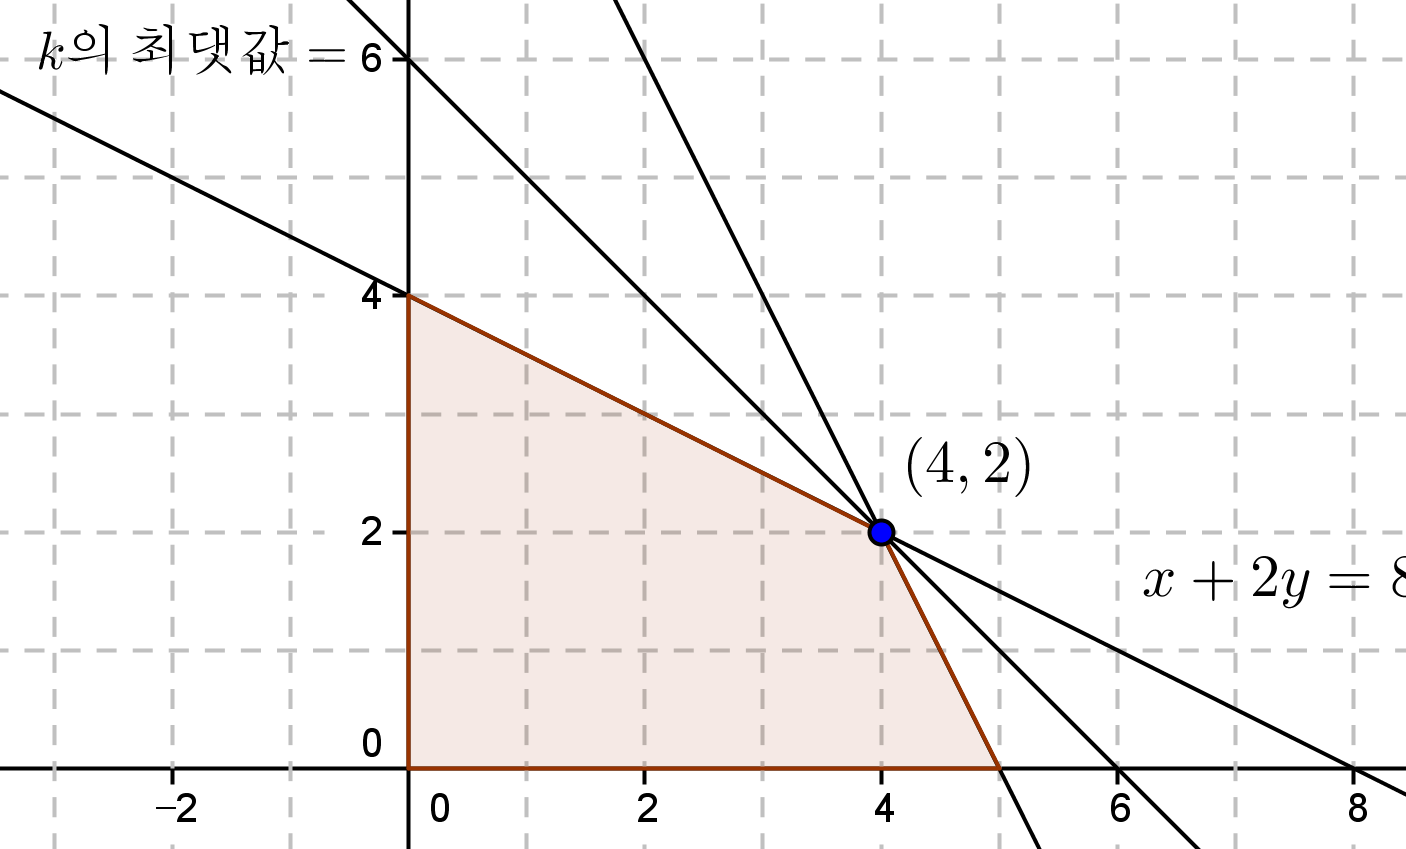
\includegraphics[width=0.5\textwidth]{range-3-3}

%
\prob{}
(1)
연립부등식
\(x\ge0\), \(2x+y\le4\), \(4x-3y\le12\)을 만족하는 \(x\), \(y\)에 대해 \(x+y\)의 최댓값과 최솟값을 구하여라.

(2)
연립부등식 \(0\le x\le 4\), \(0\le y\le 4\)를 만족하는 \(x\), \(y\)에 대해 \(y-x\)의 최댓값과 최솟값을 구하여라.

\ans{
(1) 최댓값 : \(4\), 최솟값 \(-4\)\\
(2) 최댓값 : \(4\), 최솟값 \(-4\)
}

\end{document}